\newpage
\section{Analysis and Design}

\subsection{Analysis}

\subsubsection{Business process modelling}

The three processes identified in Section 4.1.2 are modelled below as activity diagrams, one for each flow of an actor. Swimlanes separate the actor, the system, and, where it takes part, the AI model.

Exploration process. The explorer's part of the platform is modelled in seven diagrams, from access to the platform to sending feedback about the app (AD-01a to AD-01g).

\begin{figure}[H]
\centering
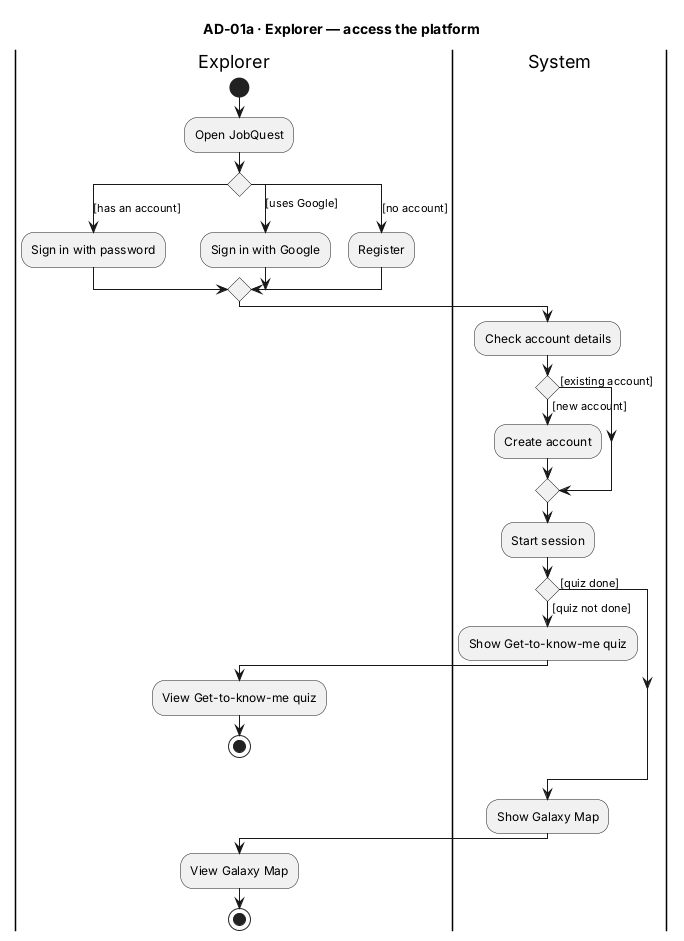
\includegraphics[width=0.62\textwidth,height=0.85\textheight,keepaspectratio]{figures/AD-01a_Explorer_AccessPlatform.png}
\caption{Explorer: access the platform (AD-01a)}
\end{figure}

\begin{figure}[H]
\centering
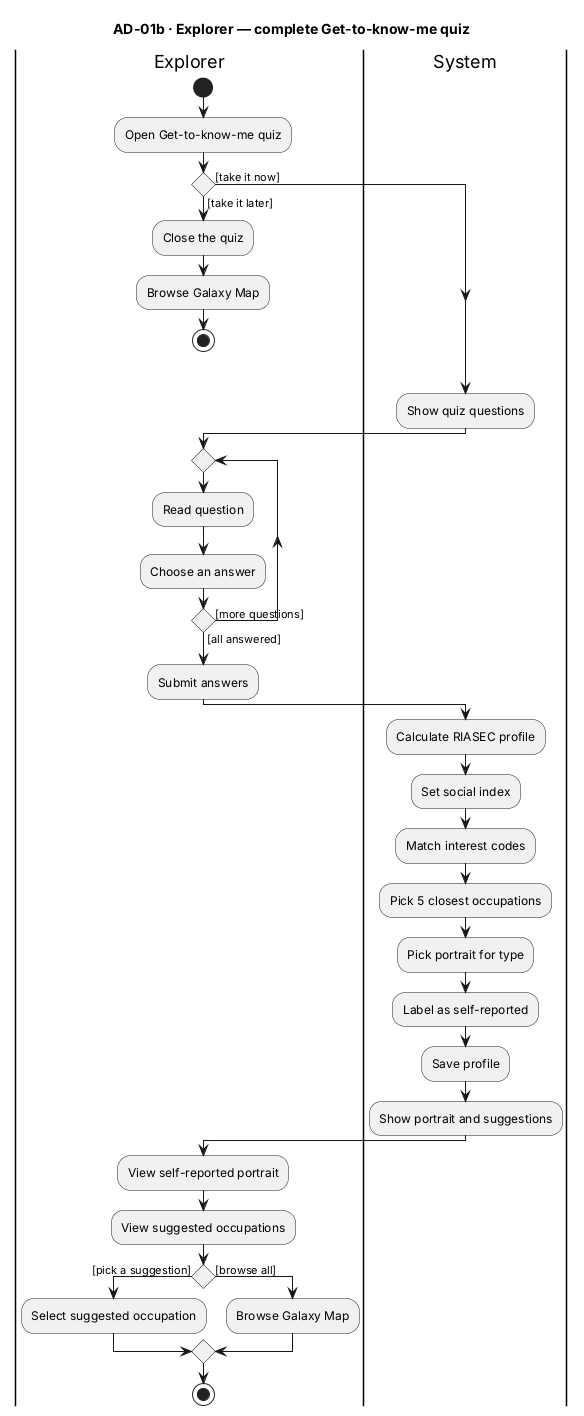
\includegraphics[width=0.53\textwidth,height=0.85\textheight,keepaspectratio]{figures/AD-01b_Explorer_GetToKnowMeQuiz.png}
\caption{Explorer: complete the Get-to-know-me quiz (AD-01b)}
\end{figure}

\begin{figure}[H]
\centering
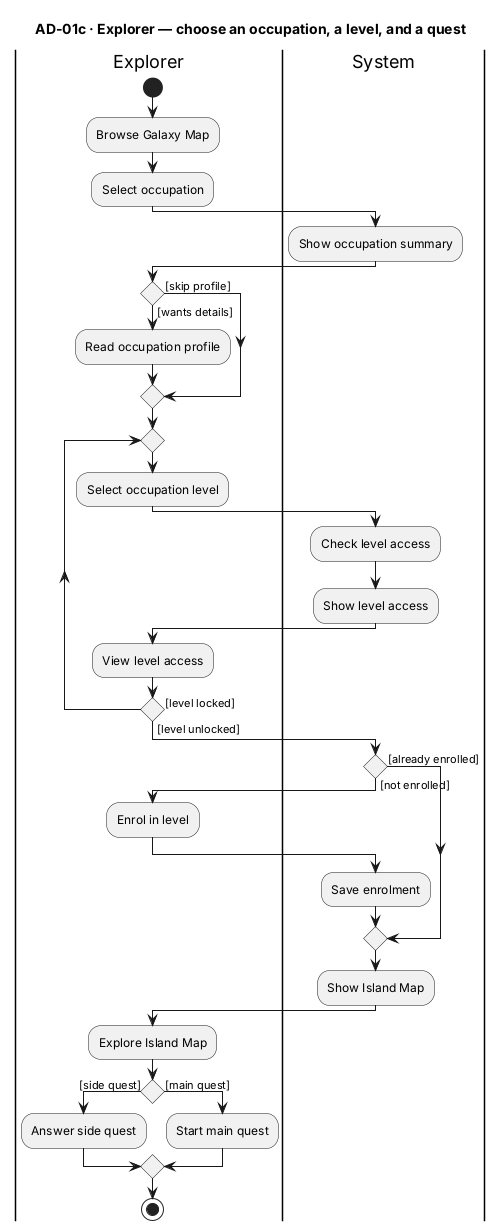
\includegraphics[width=0.46\textwidth,height=0.85\textheight,keepaspectratio]{figures/AD-01c_Explorer_ChooseLevelAndQuest.png}
\caption{Explorer: choose level and quest (AD-01c)}
\end{figure}

\begin{figure}[H]
\centering
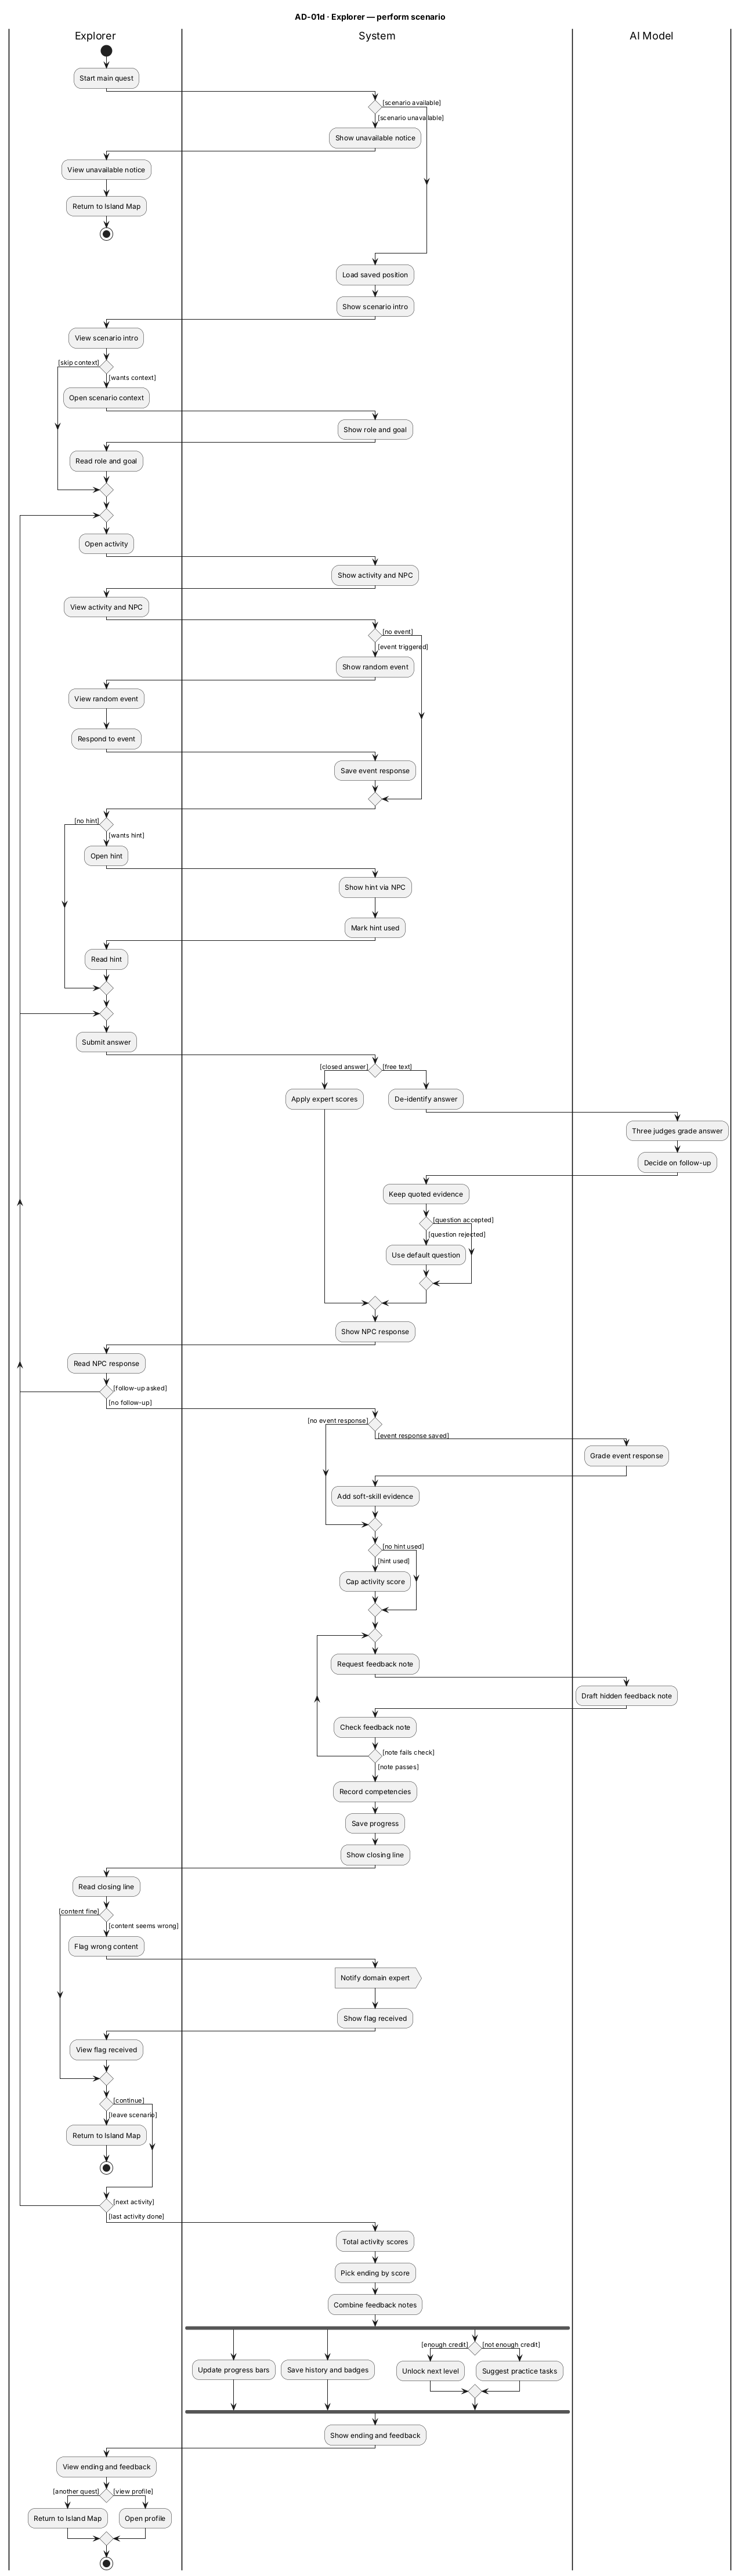
\includegraphics[width=\textwidth,height=0.85\textheight,keepaspectratio]{figures/AD-01d_Explorer_PerformScenario.png}
\caption{Explorer: perform scenario (AD-01d)}
\end{figure}

\begin{figure}[H]
\centering
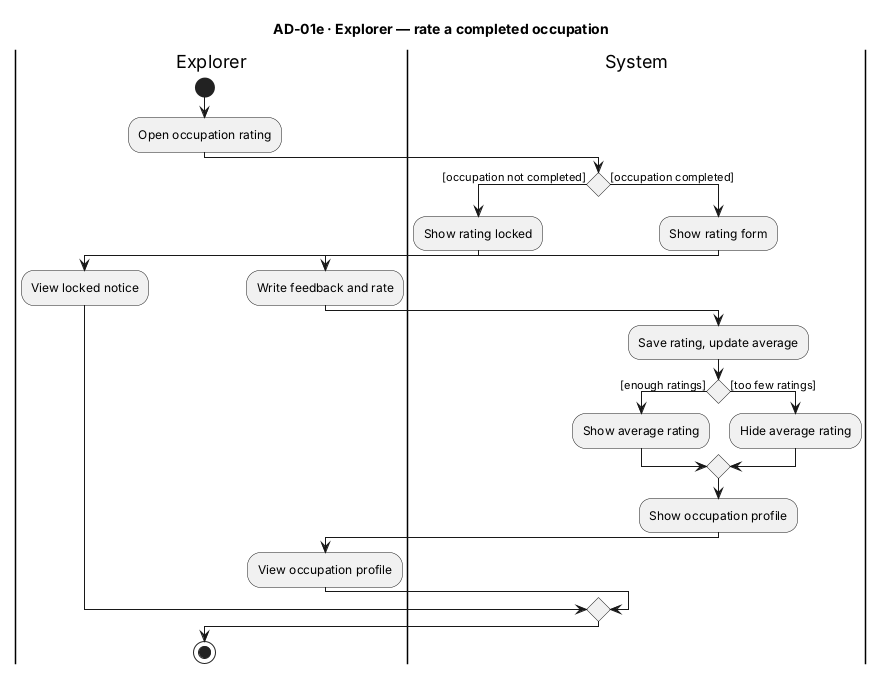
\includegraphics[width=0.8\textwidth,height=0.85\textheight,keepaspectratio]{figures/AD-01e_Explorer_RateOccupation.png}
\caption{Explorer: rate occupation (AD-01e)}
\end{figure}

\begin{figure}[H]
\centering
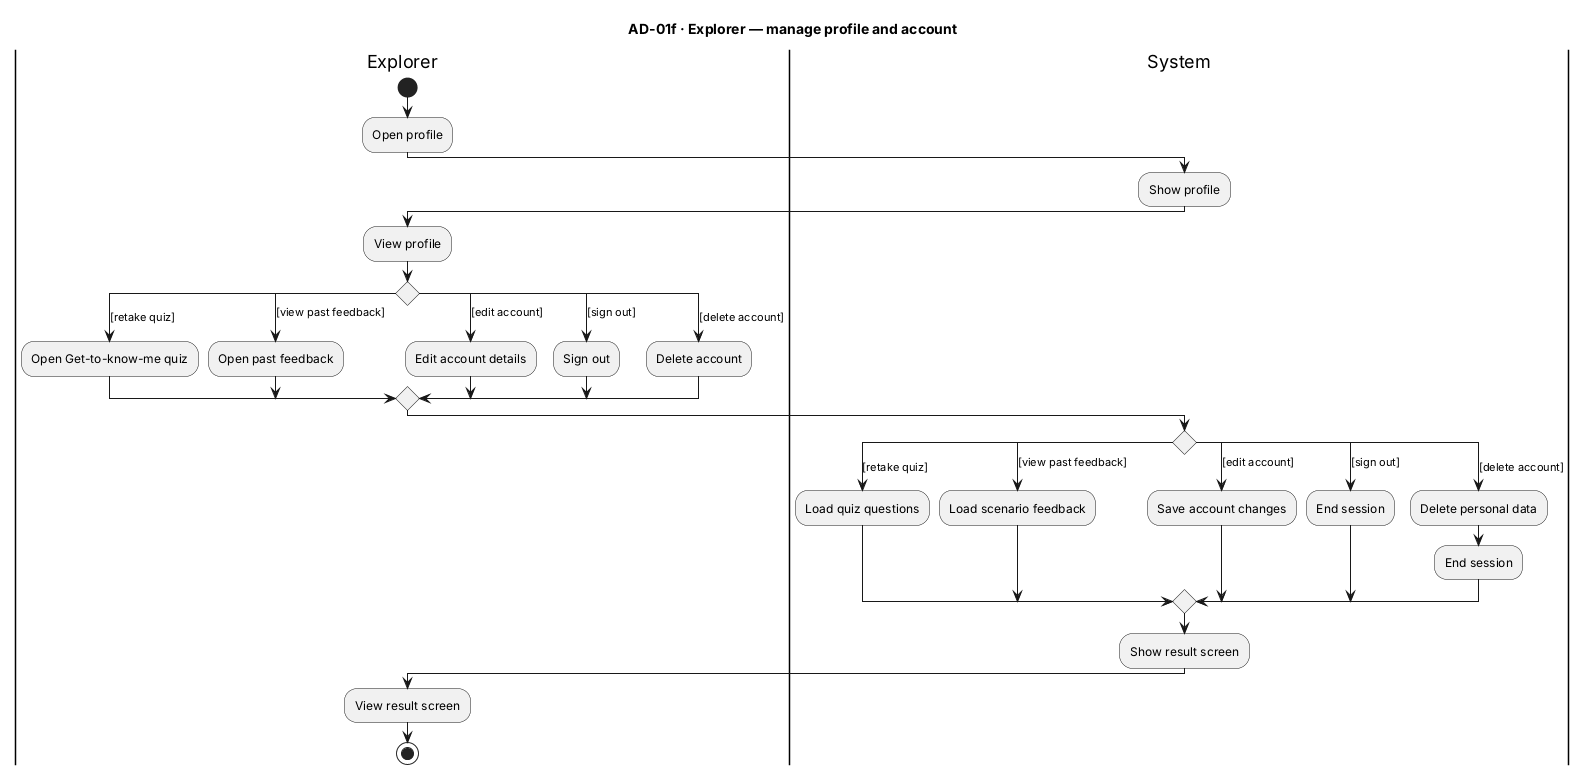
\includegraphics[width=\textwidth,height=0.85\textheight,keepaspectratio]{figures/AD-01f_Explorer_ProfileAccount.png}
\caption{Explorer: manage profile and account (AD-01f)}
\end{figure}

\begin{figure}[H]
\centering
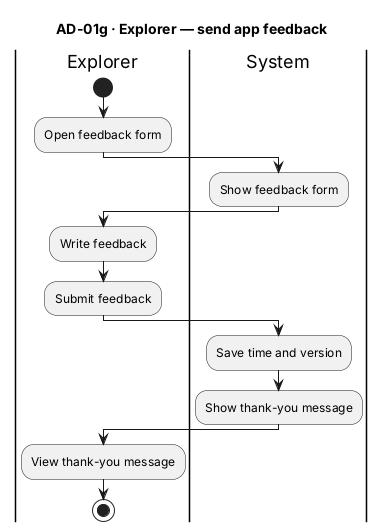
\includegraphics[width=0.35\textwidth,height=0.85\textheight,keepaspectratio]{figures/AD-01g_Explorer_SendAppFeedback.png}
\caption{Explorer: send app feedback (AD-01g)}
\end{figure}

Content lifecycle process. This process governs occupational accuracy and is the operational expression of BR-05. Domain experts author and review content in the system; the content administrator presents, publishes, and maintains it. AD-04 follows one scenario across both roles, from opening it for a task to publication; its states are those of SM-01 (Section 5.1.3).

\begin{figure}[H]
\centering
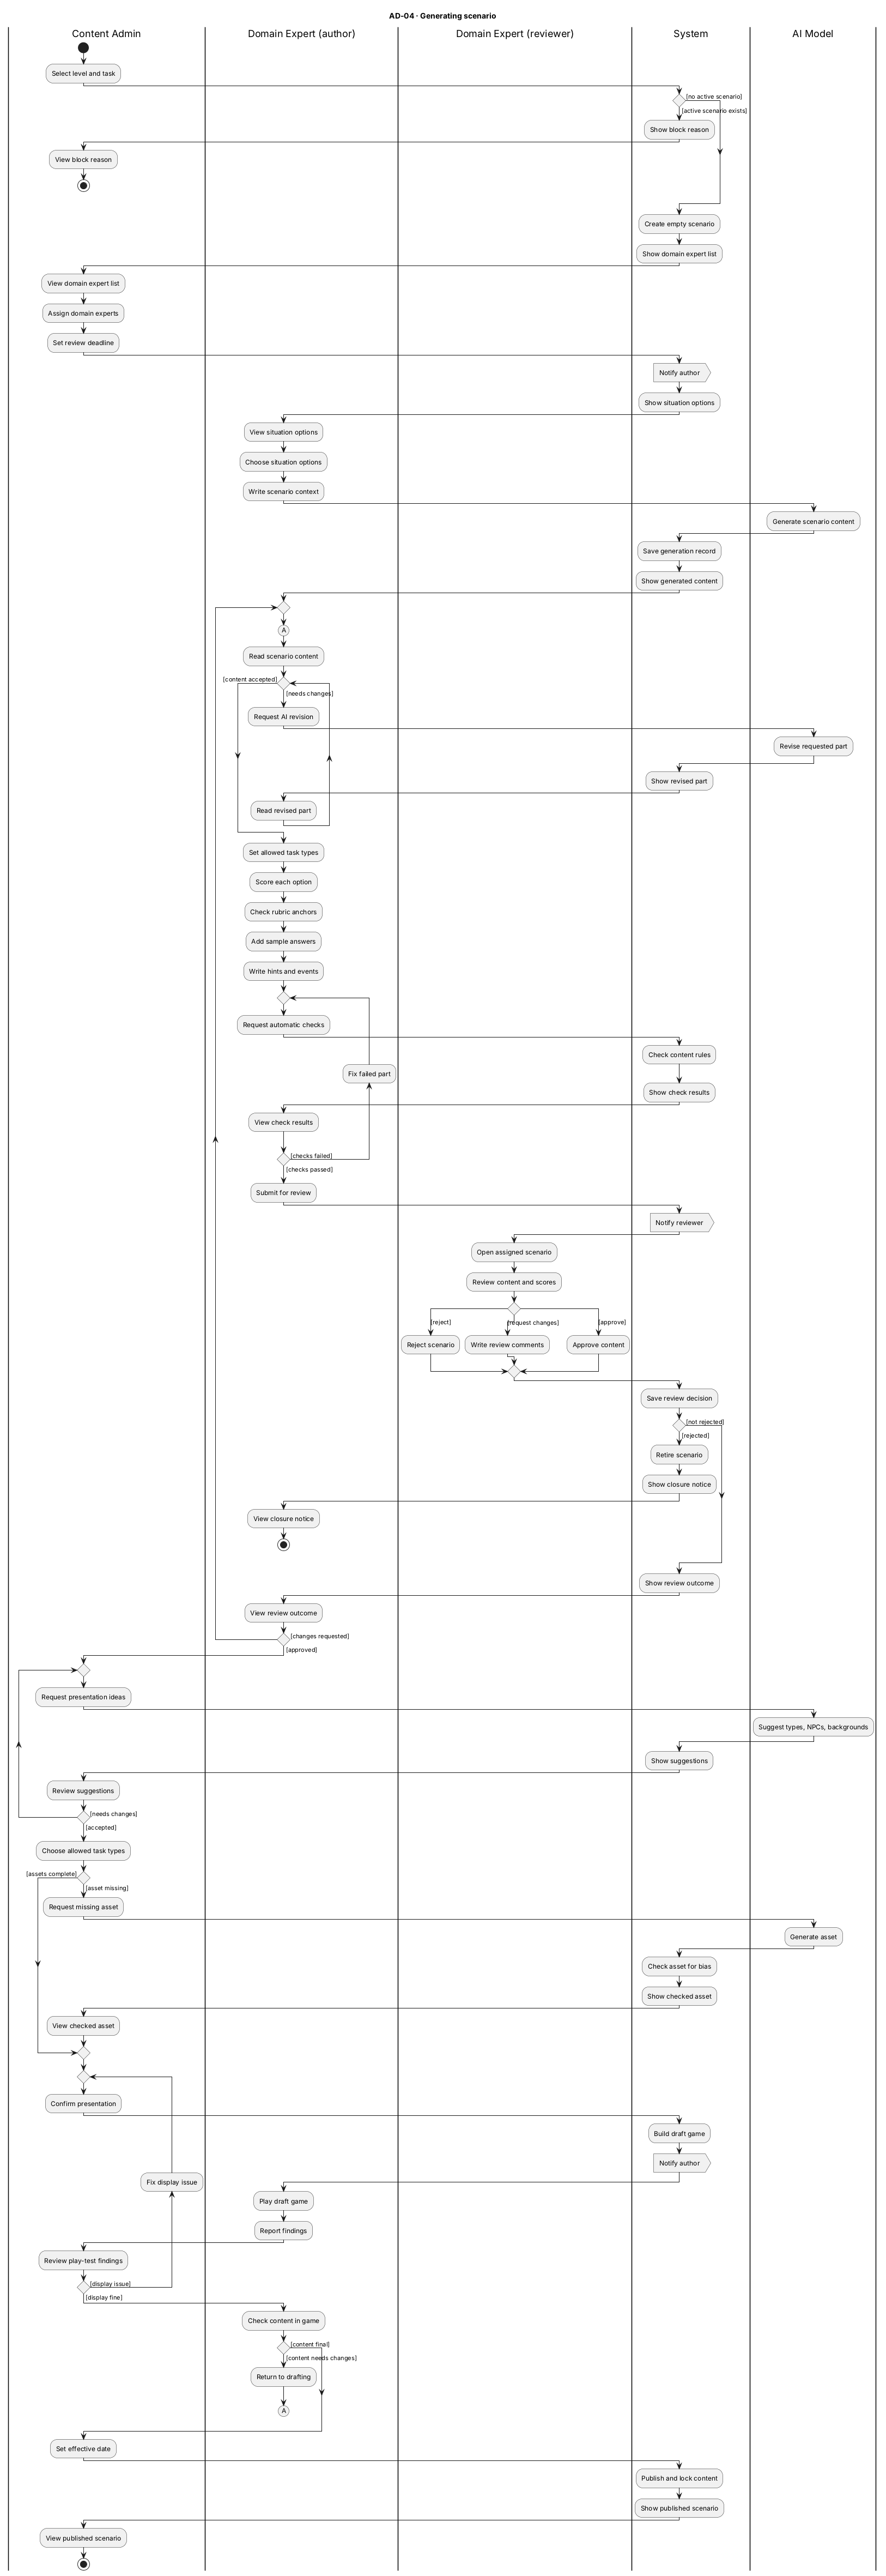
\includegraphics[width=\textwidth,height=0.85\textheight,keepaspectratio]{figures/AD-04_GeneratingScenario.png}
\caption{Scenario generation, from opening to publication (AD-04)}
\end{figure}

The content administrator's other flows are modelled in AD-02a to AD-02f.

\begin{figure}[H]
\centering
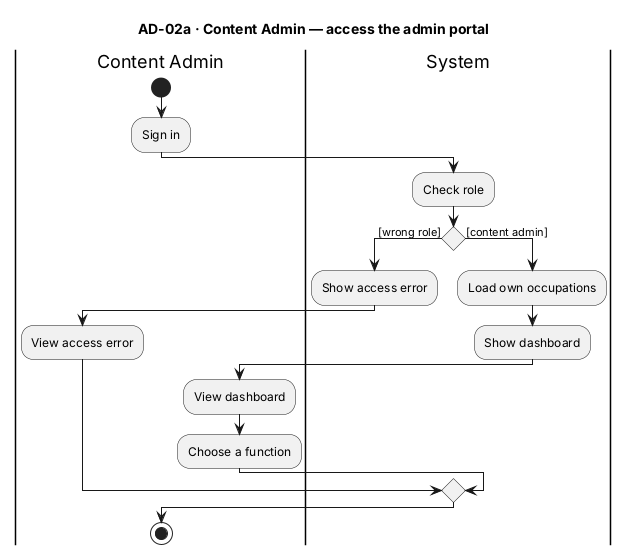
\includegraphics[width=0.57\textwidth,height=0.85\textheight,keepaspectratio]{figures/AD-02a_ContentAdmin_AccessPortal.png}
\caption{Content administrator: access the portal (AD-02a)}
\end{figure}

\begin{figure}[H]
\centering
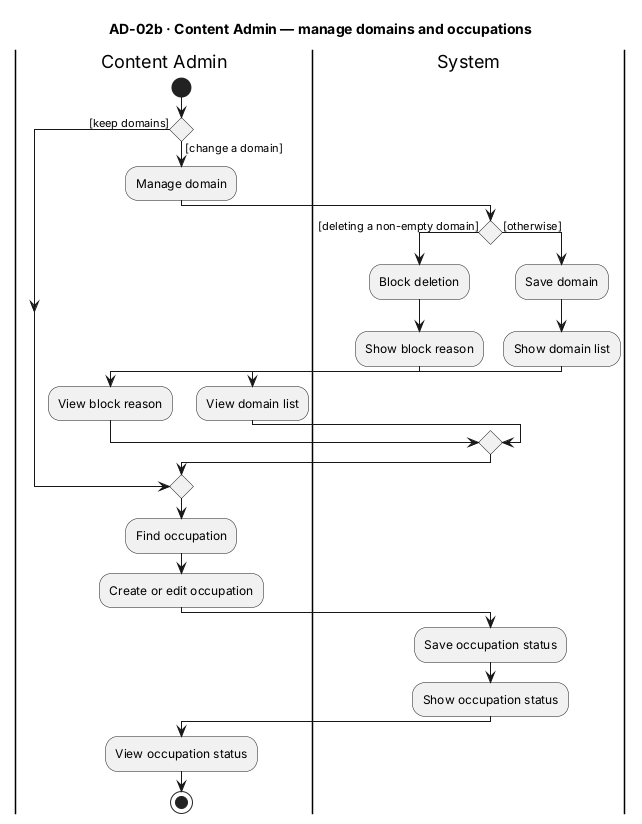
\includegraphics[width=0.58\textwidth,height=0.85\textheight,keepaspectratio]{figures/AD-02b_ContentAdmin_ManageCatalogue.png}
\caption{Content administrator: manage catalogue (AD-02b)}
\end{figure}

\begin{figure}[H]
\centering
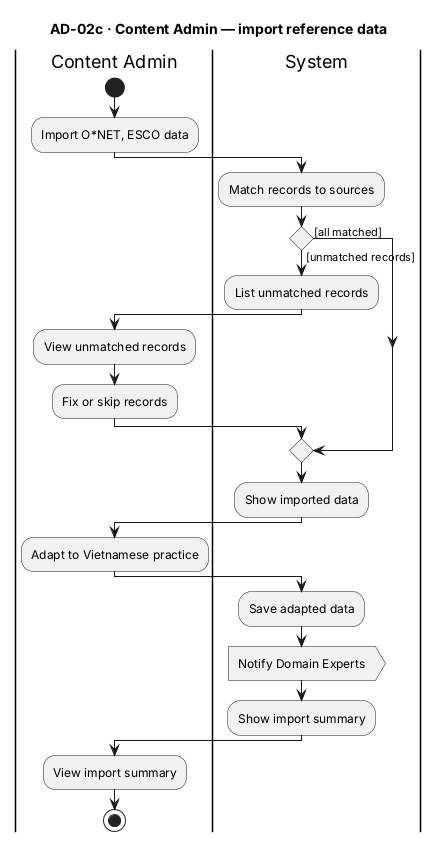
\includegraphics[width=0.4\textwidth,height=0.85\textheight,keepaspectratio]{figures/AD-02c_ContentAdmin_ImportReferenceData.png}
\caption{Content administrator: import reference data (AD-02c)}
\end{figure}

\begin{figure}[H]
\centering
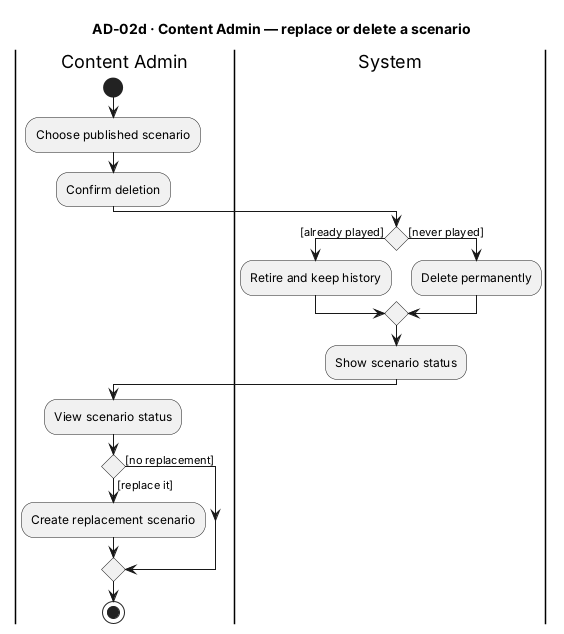
\includegraphics[width=0.51\textwidth,height=0.85\textheight,keepaspectratio]{figures/AD-02d_ContentAdmin_ReplaceOrDeleteScenario.png}
\caption{Content administrator: replace or delete scenario (AD-02d)}
\end{figure}

\begin{figure}[H]
\centering
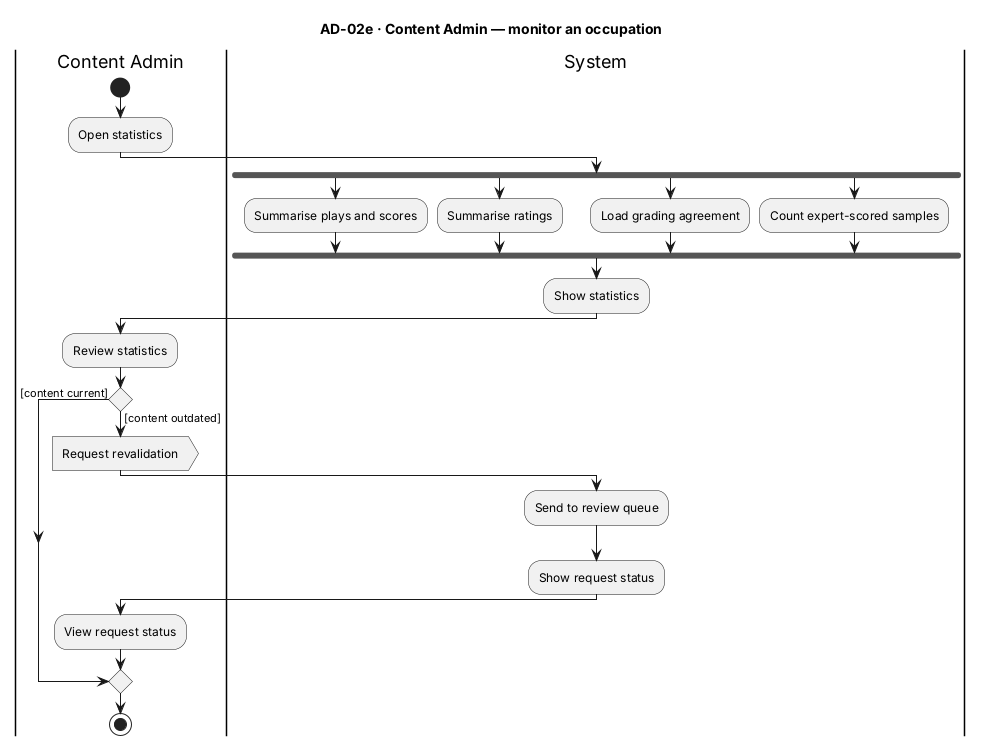
\includegraphics[width=0.89\textwidth,height=0.85\textheight,keepaspectratio]{figures/AD-02e_ContentAdmin_MonitorOccupation.png}
\caption{Content administrator: monitor occupation (AD-02e)}
\end{figure}

\begin{figure}[H]
\centering
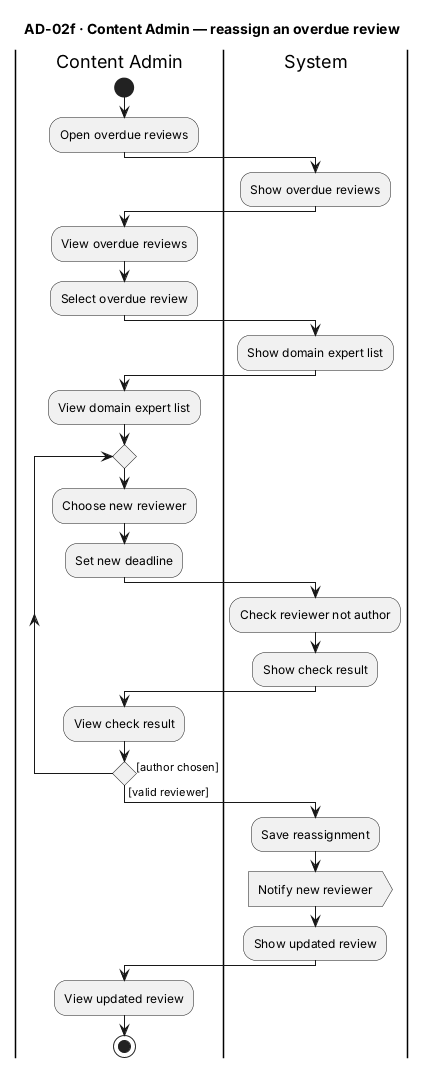
\includegraphics[width=0.39\textwidth,height=0.85\textheight,keepaspectratio]{figures/AD-02f_ContentAdmin_ReassignOverdueReview.png}
\caption{Content administrator: reassign an overdue review (AD-02f)}
\end{figure}

The domain expert's other flows are modelled in AD-03a to AD-03d.

\begin{figure}[H]
\centering
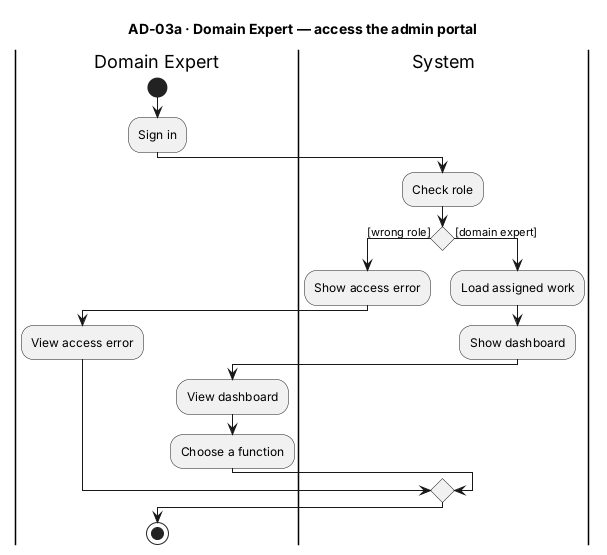
\includegraphics[width=0.55\textwidth,height=0.85\textheight,keepaspectratio]{figures/AD-03a_DomainExpert_AccessPortal.png}
\caption{Domain expert: access the portal (AD-03a)}
\end{figure}

\begin{figure}[H]
\centering
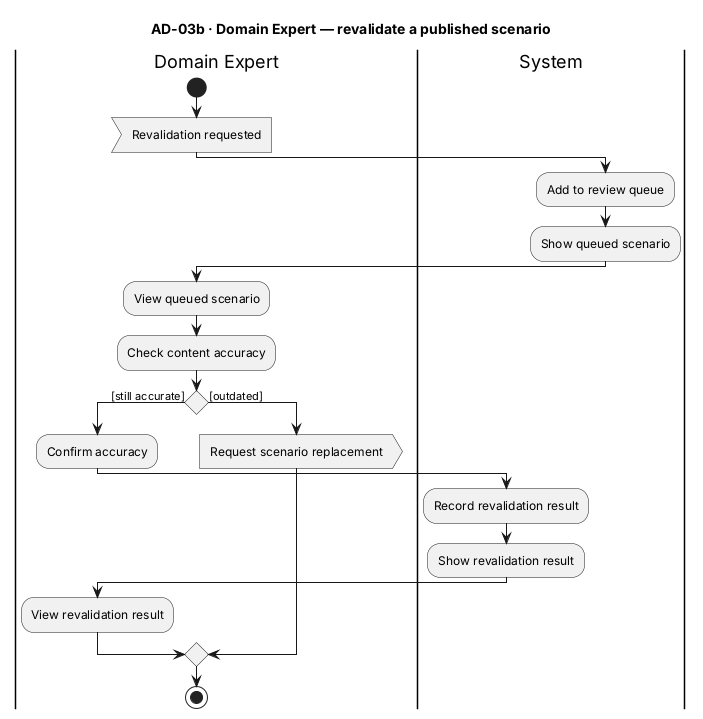
\includegraphics[width=0.64\textwidth,height=0.85\textheight,keepaspectratio]{figures/AD-03b_DomainExpert_RevalidateScenario.png}
\caption{Domain expert: revalidate scenario (AD-03b)}
\end{figure}

\begin{figure}[H]
\centering
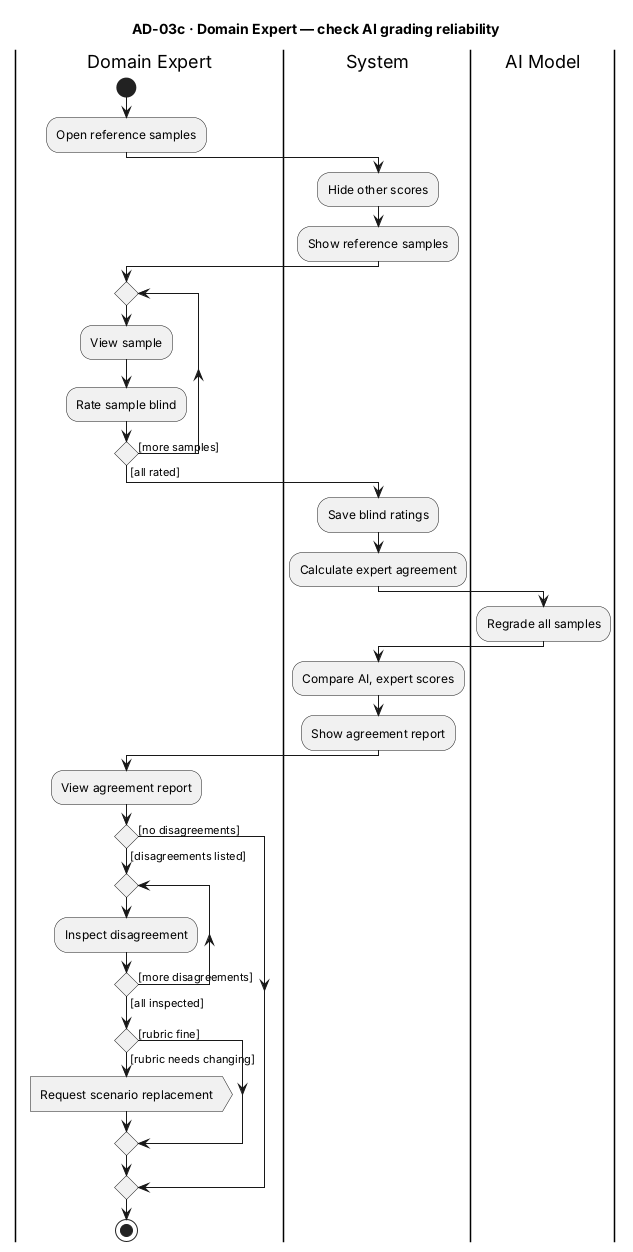
\includegraphics[width=0.58\textwidth,height=0.85\textheight,keepaspectratio]{figures/AD-03c_DomainExpert_CheckAssessorReliability.png}
\caption{Domain expert: check assessor reliability (AD-03c)}
\end{figure}

\begin{figure}[H]
\centering
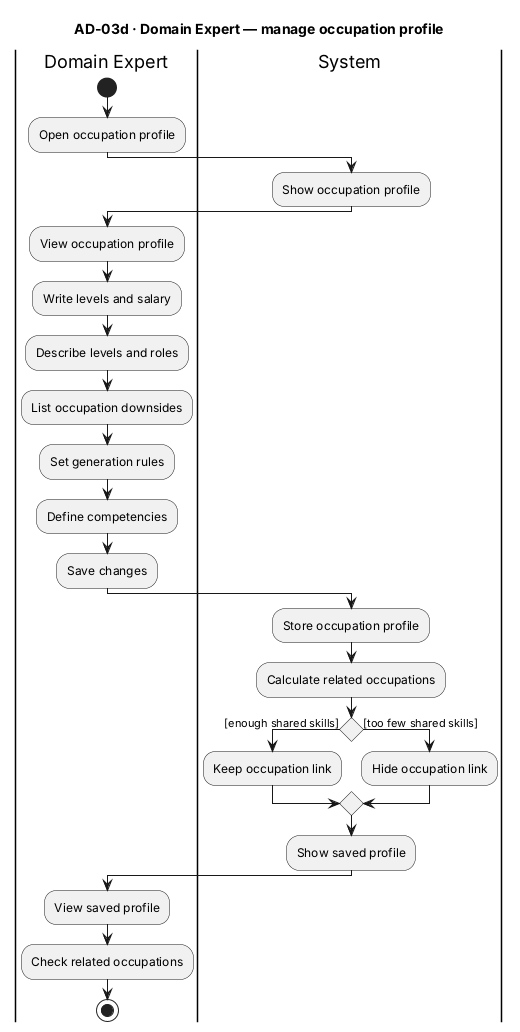
\includegraphics[width=0.47\textwidth,height=0.85\textheight,keepaspectratio]{figures/AD-03d_DomainExpert_ManageOccupationProfile.png}
\caption{Domain expert: manage occupation profile (AD-03d)}
\end{figure}

Evaluation process. This process is internal to the project and supports RP-1 and RP-2. Experts construct reference items stratified by difficulty; generation output and assessor output are compared against them; agreement is computed with chance correction and reported per stratum, together with test--retest consistency.

Platform administration. Besides the three processes, the system administrator's flows are modelled in AD-05a to AD-05e.

\begin{figure}[H]
\centering
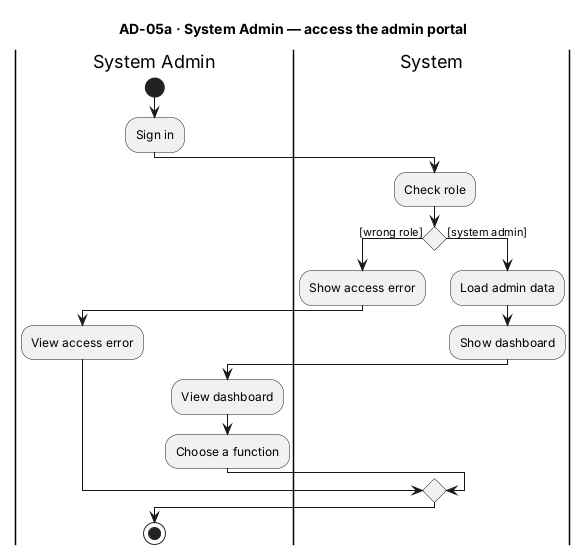
\includegraphics[width=0.53\textwidth,height=0.85\textheight,keepaspectratio]{figures/AD-05a_SystemAdmin_AccessPortal.png}
\caption{System administrator: access the portal (AD-05a)}
\end{figure}

\begin{figure}[H]
\centering
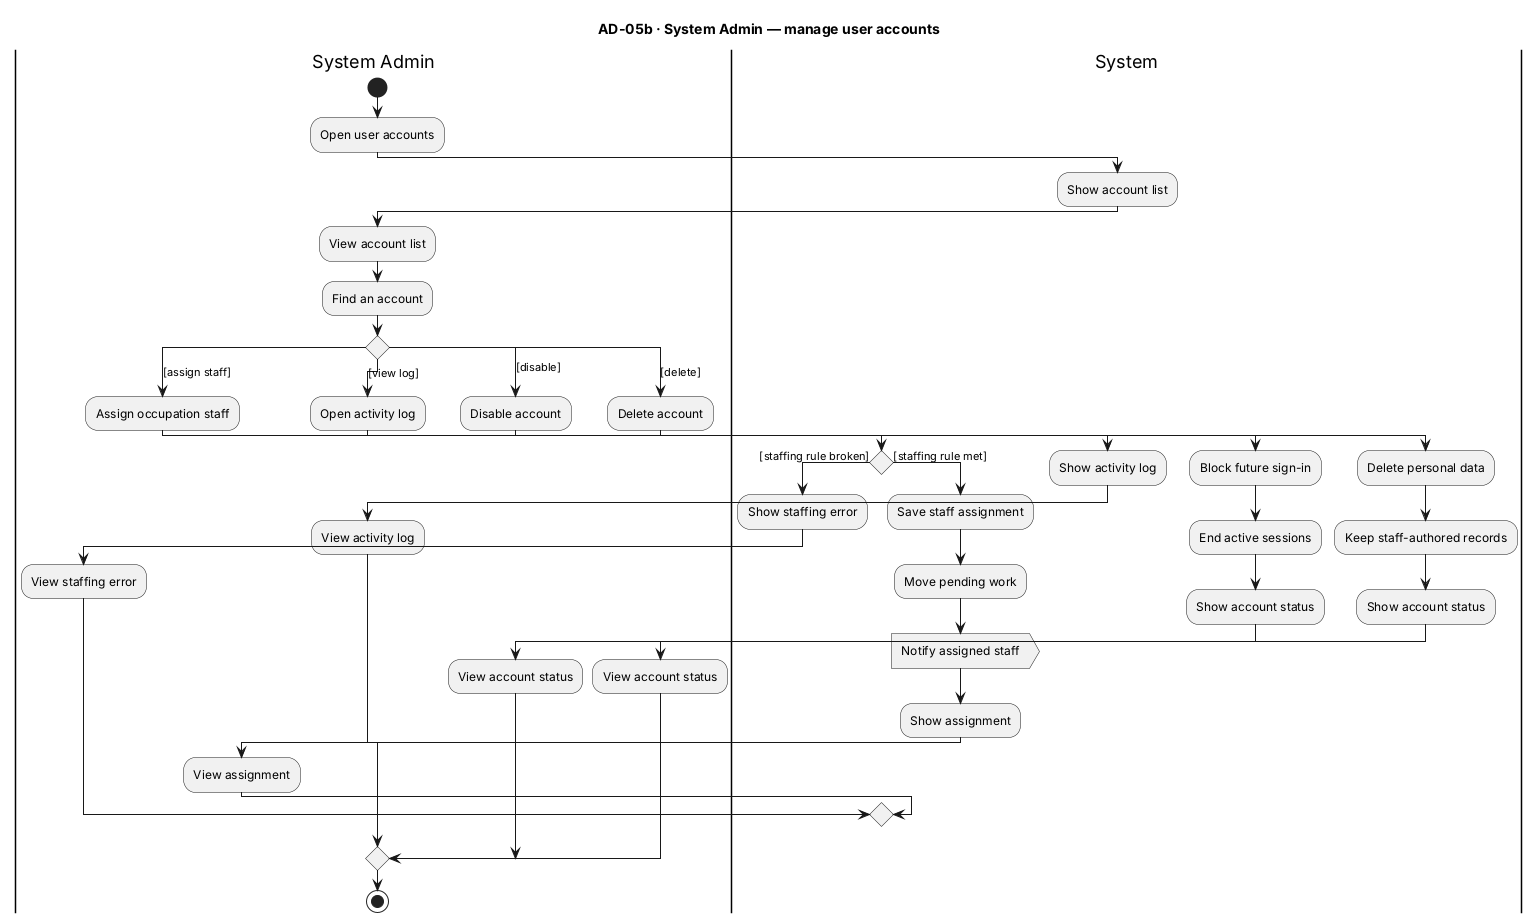
\includegraphics[width=\textwidth,height=0.85\textheight,keepaspectratio]{figures/AD-05b_SystemAdmin_ManageAccounts.png}
\caption{System administrator: manage accounts (AD-05b)}
\end{figure}

\begin{figure}[H]
\centering
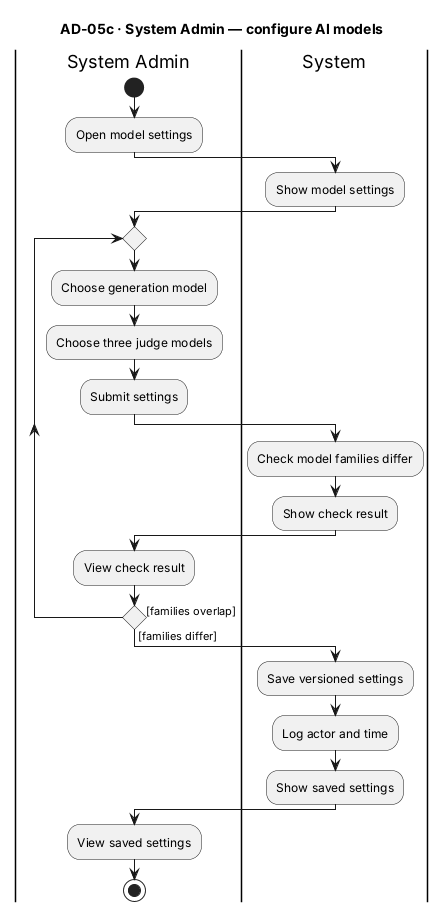
\includegraphics[width=0.41\textwidth,height=0.85\textheight,keepaspectratio]{figures/AD-05c_SystemAdmin_ConfigureModels.png}
\caption{System administrator: configure AI models (AD-05c)}
\end{figure}

\begin{figure}[H]
\centering
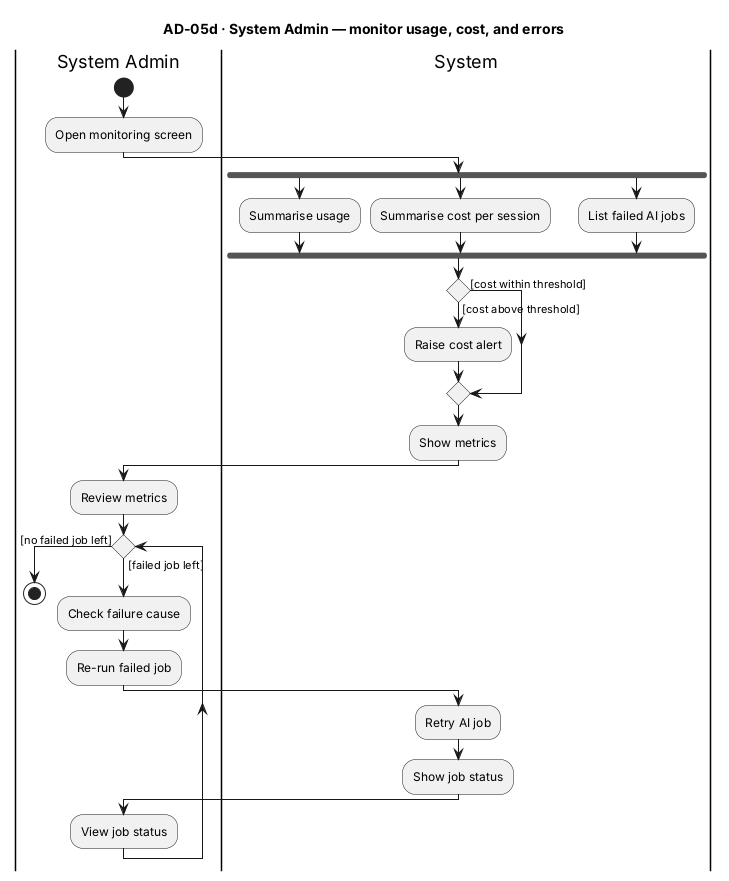
\includegraphics[width=0.66\textwidth,height=0.85\textheight,keepaspectratio]{figures/AD-05d_SystemAdmin_MonitorOperation.png}
\caption{System administrator: monitor operation (AD-05d)}
\end{figure}

\begin{figure}[H]
\centering
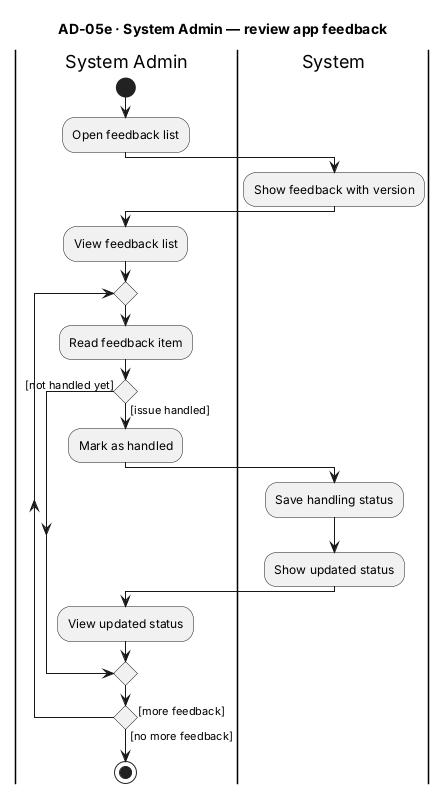
\includegraphics[width=0.41\textwidth,height=0.85\textheight,keepaspectratio]{figures/AD-05e_SystemAdmin_ReviewFeedback.png}
\caption{System administrator: review app feedback (AD-05e)}
\end{figure}

\subsubsection{Use case modelling}

Four actors correspond to the user groups in Section 4.2.1. Two external systems also participate, though they are not drawn in the diagram: the model provider, which performs generation and assessment, and the occupational data source, which supplies reference data. Use cases in the diagram are named; the descriptions below also give each an identifier by actor (UC-E for the explorer, UC-D for the domain expert, UC-C for the content administrator, and UC-S for the system administrator), and the traceability matrix refers to them by name. A use case joined to another by an include relation is always performed as part of it; one joined by an extend relation is performed only under the condition stated in the flow of the use case it extends.

\begin{figure}[H]
\centering
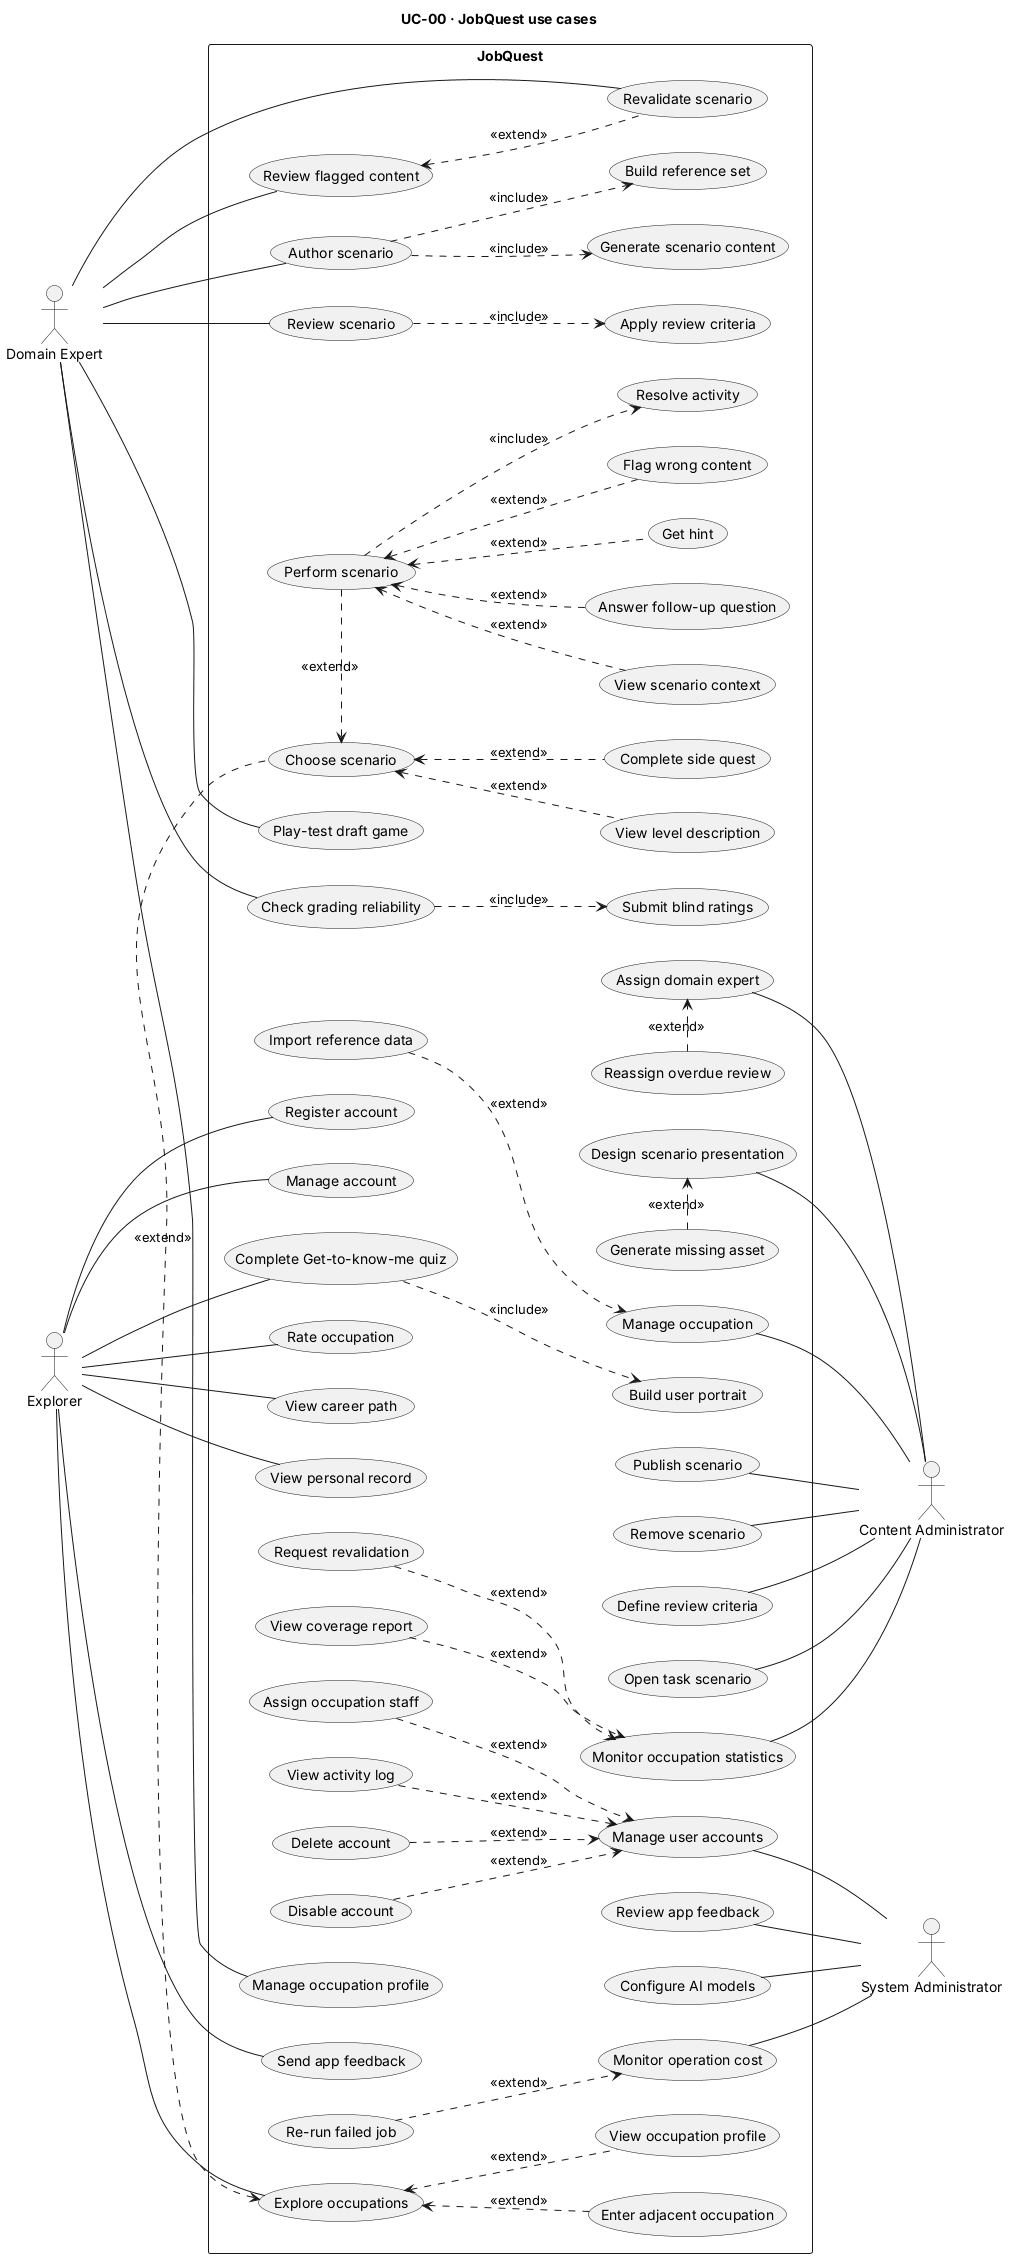
\includegraphics[width=\textwidth,height=0.9\textheight,keepaspectratio]{figures/UC-00_JobQuest.png}
\caption{Use case diagram for the proposed system (UC-00)}
\end{figure}

Use case descriptions follow, grouped by actor. Use cases associated directly with an actor, and those involving the AI model, are described in full; small included or extending use cases are described in abbreviated form. Author scenario and Review scenario are the use cases on which RP-1 depends, and Perform scenario, through Resolve activity, is the one on which RP-2 depends.

Explorer use cases.

\begin{usecase}{UC-E01}{Register account}
\ucrow{Dependencies}{%
  \ucitem{FR-01 \textit{Register, sign in with a password or Google, and recover the account}}
  \ucitem{NFR-05 \textit{Minimal, encrypted, deletable personal data}}
  \ucitem{NFR-17 \textit{Passwords hashed, traffic encrypted}}
  \ucitem{DR-16 \textit{User accounts, linked Google identities, roles, assignments, and activity log}}}
\ucrow{Description}{The system shall behave as described in the following use case when \textit{a visitor without an account creates one to start exploring}.}
\ucrow{Precondition}{\textit{The visitor has opened JobQuest and is not signed in.}}
\ucsteps{Ordinary Sequence}
\ucstep{1}{Actor \textit{visitor opens JobQuest}.}
\ucstep{2}{The system \textit{checks access and shows the sign-in screen}.}
\ucstep{3}{Actor \textit{visitor chooses to register and provides the account details}.}
\ucstep{4}{The system \textit{checks the account details and creates the account}.}
\ucstep{5}{The system \textit{starts a session}.}
\ucstep{6}{The system \textit{opens the Get-to-know-me quiz}.}
\ucrow{Postcondition}{\textit{The account exists and the explorer is signed in.}}
\ucsteps{Alternative Sequence}
\ucstep{3}{Actor \textit{visitor chooses to sign in with Google}. The system \textit{verifies the Google identity}; on the first Google sign-in it \textit{creates the account and links the Google identity to it}. The sequence \textit{continues at step 5}.}
\ucsteps{Exceptions}
\ucstep{2}{If \textit{the visitor is already signed in}, the session continues, then this use case \textit{is cancelled}.}
\ucstep{3}{If \textit{the visitor already has an account}, the visitor \textit{signs in with the password or with Google instead}, then this use case \textit{is cancelled}.}
\ucstep{6}{If \textit{the explorer has already completed the quiz}, the system \textit{opens the Galaxy Map}.}
\ucrow{Comments}{\textit{Only minimal personal data is collected and stored encrypted (NFR-05). Passwords are stored as salted hashes (NFR-17). A Google identity links to one account only (DR-16).}}
\end{usecase}

\begin{usecase}{UC-E02}{Manage account}
\ucrow{Dependencies}{%
  \ucitem{FR-02 \textit{Edit, sign out of, and delete the account}}
  \ucitem{FR-03 \textit{Retakable Get-to-know-me quiz}}
  \ucitem{FR-18 \textit{Past scenario feedback}}
  \ucitem{NFR-05 \textit{Minimal, encrypted, deletable personal data}}
  \ucitem{DR-06 \textit{User progress, including end-of-scenario feedback}}
  \ucitem{DR-16 \textit{User accounts, roles, assignments, and activity log}}}
\ucrow{Description}{The system shall behave as described in the following use case when \textit{an explorer edits, signs out of, or deletes their account, retakes the Get-to-know-me quiz, or views past feedback}.}
\ucrow{Precondition}{\textit{The explorer is signed in.}}
\ucsteps{Ordinary Sequence}
\ucstep{1}{Actor \textit{explorer opens the profile}.}
\ucstep{2}{Actor \textit{explorer opens the account settings}.}
\ucstep{3}{Actor \textit{explorer edits the account details}.}
\ucstep{4}{The system \textit{saves the changes}.}
\ucrow{Postcondition}{\textit{The account details are up to date.}}
\ucsteps{Exceptions}
\ucstep{2}{If \textit{the explorer chooses to retake the quiz}, UC-E03 \textit{Complete Get-to-know-me quiz} starts. If \textit{the explorer chooses neither}, the system \textit{opens the Galaxy Map}.}
\ucstep{2}{If \textit{the explorer chooses to view past feedback}, the system \textit{loads the end-of-scenario feedback of each past attempt and shows it}.}
\ucstep{3}{If \textit{the explorer signs out}, the system \textit{ends the session}.}
\ucstep{3}{If \textit{the explorer deletes the account}, the system \textit{deletes the personal data and ends the session}.}
\ucrow{Comments}{\textit{Account deletion removes personal data as defined in NFR-05.}}
\end{usecase}

\begin{usecase}{UC-E03}{Complete Get-to-know-me quiz}
\ucrow{Dependencies}{%
  \ucitem{FR-03 \textit{Optional, retakable RIASEC orientation quiz}}
  \ucitem{FR-04 \textit{Portrait for the RIASEC profile, including the social index}}
  \ucitem{NFR-05 \textit{Minimal, encrypted, deletable personal data}}
  \ucitem{DR-12 \textit{Quiz answers, RIASEC profile, and fixed portrait texts}}
  \ucitem{Includes UC-E04 \textit{Build user portrait}}}
\ucrow{Description}{The system shall behave as described in the following use case when \textit{an explorer takes the optional RIASEC quiz to receive occupation suggestions}.}
\ucrow{Precondition}{\textit{The explorer is signed in.}}
\ucsteps{Ordinary Sequence}
\ucstep{1}{Actor \textit{explorer opens the Get-to-know-me quiz and chooses to take it now}.}
\ucstep{2}{The system \textit{shows the quiz questions}.}
\ucstep{3}{Actor \textit{explorer answers every question and submits the answers}.}
\ucstep{4}{The system \textit{calculates the RIASEC profile}.}
\ucstep{5}{The system \textit{matches the profile with the O*NET interest code of each occupation and picks the five closest occupations}.}
\ucstep{6}{The system \textit{picks the portrait for the highest-scoring RIASEC type} (UC-E04).}
\ucstep{7}{The system \textit{saves the profile, replacing any earlier result}.}
\ucstep{8}{Actor \textit{explorer views the self-reported portrait, the social index, and the five suggested occupations}.}
\ucstep{9}{Actor \textit{explorer picks an occupation}, and the system \textit{opens it}.}
\ucrow{Postcondition}{\textit{The RIASEC profile, the portrait, and the suggestions are stored.}}
\ucsteps{Exceptions}
\ucstep{1}{If \textit{the explorer skips the quiz}, the system \textit{opens the Galaxy Map}, then this use case \textit{is cancelled}.}
\ucstep{3}{If \textit{some answers are missing}, the system \textit{highlights them}, then step 3 \textit{repeats}.}
\ucstep{9}{If \textit{the explorer chooses to browse all occupations}, the system \textit{opens the Galaxy Map}.}
\ucrow{Comments}{\textit{The quiz follows Holland's RIASEC model \cite{r41}. No AI is used in the quiz: the suggestions are computed and the portrait is selected by the system. The number of suggestions, five, is project-defined (FR-03).}}
\end{usecase}

\begin{usecase}{UC-E04}{Build user portrait}
\ucrow{Description}{The system shall behave as described in the following use case when \textit{a RIASEC profile has to be turned into a portrait}.}
\ucrow{Precondition}{\textit{The RIASEC profile has been calculated (UC-E03, step 4).}}
\ucsteps{Ordinary Sequence}
\ucstep{1}{The system \textit{takes the Social score as the social index}.}
\ucstep{2}{The system \textit{finds the highest-scoring RIASEC type of the profile}.}
\ucstep{3}{The system \textit{selects the fixed portrait text written in advance for that type}.}
\ucstep{4}{The system \textit{labels the portrait as self-reported and not validated}.}
\ucrow{Postcondition}{\textit{The portrait is stored with the profile.}}
\ucrow{Comments}{\textit{There is one portrait text for each of the six RIASEC types (FR-04, DR-12). No AI is involved, so the portrait needs no safety check.}}
\end{usecase}

\begin{usecase}{UC-E05}{Explore occupations}
\ucrow{Dependencies}{%
  \ucitem{FR-05 \textit{Galaxy Map and occupation profiles}}
  \ucitem{FR-06 \textit{Entry level open to every explorer}}
  \ucitem{DR-15 \textit{Occupation catalogue}}
  \ucitem{Extended by UC-E06, UC-E07, UC-E08}}
\ucrow{Description}{The system shall behave as described in the following use case when \textit{an explorer browses the published occupations on the Galaxy Map}.}
\ucrow{Precondition}{\textit{The explorer is signed in.}}
\ucsteps{Ordinary Sequence}
\ucstep{1}{Actor \textit{explorer opens the Galaxy Map}.}
\ucstep{2}{The system \textit{shows every published occupation}.}
\ucstep{3}{Actor \textit{explorer selects an occupation}.}
\ucstep{4}{The system \textit{opens the entry level of the occupation}.}
\ucstep{5}{The system \textit{opens the occupation map}.}
\ucstep{6}{Actor \textit{explorer reads the occupation profile} (UC-E06).}
\ucrow{Postcondition}{\textit{The explorer is on the occupation map with the entry level open.}}
\ucsteps{Exceptions}
\ucstep{3}{If \textit{an occupation has already been chosen}, for example from the quiz, the sequence \textit{continues at step 4}.}
\ucstep{4}{If \textit{the explorer's competencies overlap with this occupation}, UC-E07 \textit{Enter adjacent occupation} runs.}
\ucstep{6}{Actor \textit{explorer may skip the profile and choose a level} (UC-E08).}
\ucrow{Comments}{\textit{The entry level opens with zero credit and without any adjacency check (FR-06).}}
\end{usecase}

\begin{usecase}{UC-E06}{View occupation profile}
\ucrow{Description}{The system shall behave as described in the following use case when \textit{an explorer reads the profile of the selected occupation}.}
\ucrow{Precondition}{\textit{An occupation is selected.}}
\ucsteps{Ordinary Sequence}
\ucstep{1}{Actor \textit{explorer chooses to read the profile}.}
\ucstep{2}{The system \textit{shows all profile fields, the main downsides, and a description of every level}.}
\ucstep{3}{The system \textit{shows the average rating if enough ratings exist}.}
\ucrow{Postcondition}{\textit{The explorer returns to the occupation map.}}
\end{usecase}

\begin{usecase}{UC-E07}{Enter adjacent occupation}
\ucrow{Description}{The system shall behave as described in the following use case when \textit{the explorer's recorded competencies overlap with the selected occupation}.}
\ucrow{Precondition}{\textit{An occupation is selected, and the explorer has recorded competencies.}}
\ucsteps{Ordinary Sequence}
\ucstep{1}{The system \textit{compares the explorer's competencies with the adjacency data of the occupation}.}
\ucstep{2}{The system \textit{unlocks a higher starting level if the overlap conditions are met}.}
\ucstep{3}{The system \textit{keeps the entry level open}.}
\ucrow{Postcondition}{\textit{The explorer can start at the entry level or at the unlocked level.}}
\end{usecase}

\begin{usecase}{UC-E08}{Choose scenario}
\ucrow{Dependencies}{%
  \ucitem{FR-08 \textit{Enrol in levels, choose scenarios, unlock the next level}}
  \ucitem{FR-33 \textit{One active scenario per task}}
  \ucitem{DR-06 \textit{User progress}}
  \ucitem{Includes UC-E09; extended by UC-E10; extends UC-E05}}
\ucrow{Description}{The system shall behave as described in the following use case when \textit{an explorer chooses a level, enrols in it, and picks a quest}.}
\ucrow{Precondition}{\textit{The explorer is on the occupation map.}}
\ucsteps{Ordinary Sequence}
\ucstep{1}{Actor \textit{explorer chooses a level}.}
\ucstep{2}{The system \textit{shows the level description} (UC-E09).}
\ucstep{3}{The system \textit{confirms that the level is unlocked}.}
\ucstep{4}{Actor \textit{explorer enrols in the level}.}
\ucstep{5}{The system \textit{saves the enrolment}.}
\ucstep{6}{The system \textit{opens the Island Map}.}
\ucstep{7}{Actor \textit{explorer chooses a main quest}, then UC-E11 \textit{Perform scenario} starts.}
\ucrow{Postcondition}{\textit{The explorer is enrolled in the level and has chosen a scenario.}}
\ucsteps{Exceptions}
\ucstep{3}{If \textit{the level is locked}, the system \textit{shows the required credit}, then step 1 \textit{repeats}.}
\ucstep{4}{If \textit{the explorer is already enrolled}, the sequence \textit{continues at step 6}.}
\ucstep{7}{If \textit{the explorer chooses a side quest}, UC-E10 \textit{Complete side quest} runs.}
\ucrow{Comments}{\textit{A task has at most one active scenario (FR-33), so choosing a quest means choosing a task.}}
\end{usecase}

\begin{usecase}{UC-E09}{View level description}
\ucrow{Description}{The system shall behave as described in the following use case when \textit{an explorer chooses a level}.}
\ucrow{Precondition}{\textit{The explorer is on the occupation map.}}
\ucsteps{Ordinary Sequence}
\ucstep{1}{The system \textit{shows what the level involves and the credit needed to unlock it}.}
\ucrow{Postcondition}{\textit{The explorer knows what the level involves.}}
\end{usecase}

\begin{usecase}{UC-E10}{Complete side quest}
\ucrow{Description}{The system shall behave as described in the following use case when \textit{an explorer answers a side quest on the Island Map}.}
\ucrow{Precondition}{\textit{The explorer is enrolled in the level and is on the Island Map.}}
\ucsteps{Ordinary Sequence}
\ucstep{1}{Actor \textit{explorer chooses a side quest}.}
\ucstep{2}{Actor \textit{explorer answers the quick question}.}
\ucstep{3}{The system \textit{adds bonus points, recorded separately from competence credit}.}
\ucrow{Postcondition}{\textit{The bonus points are recorded.}}
\end{usecase}

\begin{usecase}{UC-E11}{Perform scenario}
\ucrow{Dependencies}{%
  \ucitem{FR-09 \textit{Offer role, team, and context before each scenario}}
  \ucitem{FR-10, FR-11 \textit{Answer forms and anchored scoring by three judges}}
  \ucitem{FR-13, FR-14, FR-15 \textit{Hints, checked feedback notes, and recorded competencies}}
  \ucitem{NFR-03, NFR-04 \textit{Progress survives interruption and provider failure}}
  \ucitem{NFR-05, NFR-07 \textit{De-identified data; AI disclosure}}
  \ucitem{DR-06, DR-07 \textit{User progress; assessment records}}
  \ucitem{Includes UC-E13; extended by UC-E12, UC-E14, UC-E15, UC-E16; extends UC-E08}}
\ucrow{Description}{The system shall behave as described in the following use case when \textit{an explorer plays a published scenario of a level they are enrolled in}.}
\ucrow{Precondition}{\textit{The explorer is signed in, is enrolled in the level, and has chosen a main quest (UC-E08).}}
\ucsteps{Ordinary Sequence}
\ucstep{1}{The system \textit{checks that the scenario is available, loads it at the saved position, and shows the scenario intro}.}
\ucstep{2}{Actor \textit{explorer reads the intro and may open the scenario context} (UC-E12).}
\ucstep{3}{The system \textit{opens the activity and shows the NPC line}.}
\ucstep{4}{Actor \textit{explorer submits an answer}.}
\ucstep{5}{The system \textit{resolves the activity} (UC-E13).}
\ucstep{6}{The system \textit{requests a feedback note for the activity}.}
\ucstep{7}{The AI model \textit{drafts the hidden feedback note from the rubric anchors}.}
\ucstep{8}{The system \textit{checks the feedback note}.}
\ucstep{9}{The system \textit{records the competencies, saves progress, and shows the NPC closing line}.}
\ucstep{10}{Steps 3--9 \textit{repeat for each remaining activity}.}
\ucstep{11}{The system \textit{totals the activity scores and picks the ending that matches the total}.}
\ucstep{12}{The system \textit{combines the feedback notes into the end-of-scenario feedback}.}
\ucstep{13}{The system \textit{updates the progress bars, saves the play history and badges, and unlocks the next level if the credit reaches the threshold}.}
\ucstep{14}{Actor \textit{explorer views the ending, the feedback, and the guidance, then returns to the Island Map}.}
\ucrow{Postcondition}{\textit{The evidence, feedback notes, progress, and play history are stored, and the explorer has received the ending, feedback, and guidance.}}
\ucsteps{Exceptions}
\ucstep{1}{If \textit{the scenario is not available}, the system \textit{shows a notice}, and actor \textit{explorer returns to the Island Map}, then this use case \textit{is cancelled}.}
\ucstep{3}{If \textit{a random event is triggered}, the system \textit{shows it}, actor \textit{explorer responds}, and the AI model \textit{grades the response as bonus soft-skill evidence}. The sequence \textit{continues at step 4}.}
\ucstep{4}{Actor \textit{explorer may open a hint} (UC-E15). The +2 mark of the activity \textit{is then lowered to 0}.}
\ucstep{5}{If \textit{the free-text answer needs a follow-up and the limit has not been reached}, UC-E14 \textit{Answer follow-up question} runs.}
\ucstep{8}{If \textit{the feedback note fails the check}, the AI model \textit{redrafts the note}, then step 8 \textit{repeats}.}
\ucstep{9}{If \textit{the content seems wrong}, actor \textit{explorer flags it} (UC-E16).}
\ucstep{9}{If \textit{the explorer leaves the scenario}, the system \textit{has saved progress and returns to the Island Map}. The scenario \textit{later resumes at the saved position}.}
\ucstep{13}{If \textit{the credit is not enough}, the system \textit{suggests tasks to practise}.}
\ucstep{14}{Actor \textit{explorer may open the profile instead}.}
\ucrow{Comments}{\textit{AI-written follow-ups must pass the output check, otherwise the expert's default follow-up is shown (FR-12). Feedback notes must pass the output check, otherwise they are redrafted; there is no expert default for feedback (FR-14). Credit is capped per skill per scenario, so replaying never inflates it (FR-15). Random-event answers add bonus soft-skill evidence only and never lower the main score (FR-15, FR-22).}}
\end{usecase}

\begin{usecase}{UC-E12}{View scenario context}
\ucrow{Description}{The system shall behave as described in the following use case when \textit{an explorer chooses to read the full context of a scenario from its intro}.}
\ucrow{Precondition}{\textit{The scenario intro is shown (UC-E11, step 1).}}
\ucsteps{Ordinary Sequence}
\ucstep{1}{Actor \textit{explorer opens the scenario context}.}
\ucstep{2}{The system \textit{shows the role, the team, the goal, and the working context}.}
\ucstep{3}{Actor \textit{explorer reads the role and goal}.}
\ucrow{Postcondition}{\textit{The explorer returns to the scenario, before the first activity.}}
\ucrow{Comments}{\textit{The intro is always shown; the full context is optional, and an explorer who skips it goes straight to the first activity (FR-09).}}
\end{usecase}

\begin{usecase}{UC-E13}{Resolve activity}
\ucrow{Dependencies}{%
  \ucitem{FR-10 \textit{Choice, ordering, prioritising, and free-text answers}}
  \ucitem{FR-11 \textit{Anchored scoring by three judges, backed by quotations}}
  \ucitem{FR-12 \textit{Follow-up decided after grading}}
  \ucitem{FR-13, FR-15 \textit{Hint penalty; capped competencies}}
  \ucitem{NFR-02, NFR-04, NFR-05, NFR-14, NFR-17}
  \ucitem{DR-07 \textit{Assessment records, including each judge's score and the combined grade}}
  \ucitem{Included by UC-E11 and UC-E14}}
\ucrow{Description}{The system shall behave as described in the following use case when \textit{an answer submitted by the explorer has to be scored}.}
\ucrow{Precondition}{\textit{The explorer has submitted an answer to an activity.}}
\ucsteps{Ordinary Sequence}
\ucstep{1}{The system \textit{checks the answer type}.}
\ucstep{2}{The system \textit{de-identifies the free-text answer}.}
\ucstep{3}{The system \textit{sends the answer to three AI judges in parallel as separated data, together with the rubric anchors}.}
\ucstep{4}{Each AI judge \textit{grades the answer against the anchors, quoting the explorer's words}.}
\ucstep{5}{The system \textit{checks that every quotation appears verbatim in the answer and that every score is a rubric anchor}.}
\ucstep{6}{The system \textit{combines the three judges' scores into one grade and keeps the evidence with the exact quotations}.}
\ucstep{7}{The AI model \textit{decides, from the graded answer, whether a follow-up is needed}.}
\ucstep{8}{The system \textit{shows the NPC response}.}
\ucrow{Postcondition}{\textit{Each judge's score, the combined grade, and the evidence are stored with their quotations.}}
\ucsteps{Exceptions}
\ucstep{1}{If \textit{the answer is a choice, ordering, or prioritising answer}, the system \textit{scores it with the expert's scores}, then the sequence \textit{continues at step 8}.}
\ucstep{4}{If \textit{a judge model fails}, the system \textit{switches to another available model of the same family}. If \textit{no model is available}, the system \textit{keeps the progress and notifies the explorer within 10\,s} (NFR-04).}
\ucstep{5}{If \textit{a quotation is not found or a score is outside the anchors}, the system \textit{rejects that judge's result}.}
\ucstep{7}{If \textit{a follow-up is needed and the limit has not been reached}, UC-E14 \textit{Answer follow-up question} runs.}
\ucstep{8}{If \textit{a hint was used in this activity}, the system \textit{lowers +2 to 0}.}
\ucrow{Comments}{\textit{Every answer, follow-up answers included, is graded as soon as it is submitted and before any follow-up is decided (FR-11, FR-12). Free-text assessment finishes within 8\,s at the 95th percentile (NFR-02). Instructions written inside an answer are ignored (NFR-17). Agreement with experts is checked under NFR-14.}}
\end{usecase}

\begin{usecase}{UC-E14}{Answer follow-up question}
\ucrow{Dependencies}{%
  \ucitem{FR-12 \textit{AI-generated follow-up questions}}
  \ucitem{NFR-01 \textit{Follow-up generation time}}
  \ucitem{NFR-15 \textit{AI content stays within expert-set limits}}
  \ucitem{Extends UC-E11; includes UC-E13}}
\ucrow{Description}{The system shall behave as described in the following use case when \textit{the AI model probes a free-text answer further}.}
\ucrow{Precondition}{\textit{A free-text answer has been graded by the three judges (UC-E13), a follow-up is needed, and the follow-up limit of the activity has not been reached.}}
\ucsteps{Ordinary Sequence}
\ucstep{1}{The AI model \textit{generates a follow-up question within the expert's follow-up goal}.}
\ucstep{2}{The system \textit{runs the output check}.}
\ucstep{3}{The system \textit{shows the follow-up question}.}
\ucstep{4}{Actor \textit{explorer answers the follow-up question}.}
\ucstep{5}{The system \textit{has the three judges grade the follow-up answer} (UC-E13).}
\ucstep{6}{Steps 1--5 \textit{repeat while the graded answer calls for a follow-up and the limit has not been reached}.}
\ucrow{Postcondition}{\textit{The follow-up answers are stored with each judge's score, the combined grade, and their evidence.}}
\ucsteps{Exceptions}
\ucstep{1}{If \textit{generation takes longer than 2\,s}, the system \textit{shows progress} (NFR-01).}
\ucstep{2}{If \textit{the output check fails or the provider returns an error}, the system \textit{shows the expert's default follow-up instead}.}
\ucrow{Comments}{\textit{Follow-ups are generated within 5\,s at the 95th percentile (NFR-01), and only for free-text answers.}}
\end{usecase}

\begin{usecase}{UC-E15}{Get hint}
\ucrow{Description}{The system shall behave as described in the following use case when \textit{an explorer opens a hint during an activity}.}
\ucrow{Precondition}{\textit{The current activity has a hint.}}
\ucsteps{Ordinary Sequence}
\ucstep{1}{Actor \textit{explorer opens the hint}.}
\ucstep{2}{The system \textit{shows the hint as an NPC line}.}
\ucstep{3}{The system \textit{records the hint use and removes the +2 mark for this activity}.}
\ucrow{Postcondition}{\textit{The hint use is recorded and shown in the summary.}}
\end{usecase}

\begin{usecase}{UC-E16}{Flag wrong content}
\ucrow{Description}{The system shall behave as described in the following use case when \textit{an explorer reports wrong content in a scenario}.}
\ucrow{Precondition}{\textit{The explorer is in a scenario or is viewing its feedback.}}
\ucsteps{Ordinary Sequence}
\ucstep{1}{Actor \textit{explorer flags the content}.}
\ucstep{2}{The system \textit{stores the flag with the assessment record}.}
\ucstep{3}{The system \textit{sends the flag to a domain expert of the occupation} (UC-D07).}
\ucrow{Postcondition}{\textit{The flag has reached a domain expert.}}
\end{usecase}

\begin{usecase}{UC-E17}{Rate occupation}
\ucrow{Dependencies}{%
  \ucitem{FR-19 \textit{Collect occupation ratings and feedback}}
  \ucitem{NFR-06 \textit{Suppress aggregates below a minimum population}}
  \ucitem{DR-08 \textit{Five-attribute occupation ratings}}}
\ucrow{Description}{The system shall behave as described in the following use case when \textit{an explorer rates an occupation after completing it}.}
\ucrow{Precondition}{\textit{The explorer has completed every level of the occupation.}}
\ucsteps{Ordinary Sequence}
\ucstep{1}{Actor \textit{explorer opens the occupation rating}.}
\ucstep{2}{The system \textit{confirms that the occupation is completed}.}
\ucstep{3}{Actor \textit{explorer writes feedback and rates the occupation}.}
\ucstep{4}{The system \textit{saves the rating and updates the average}.}
\ucstep{5}{The system \textit{shows the ratings of other explorers}.}
\ucstep{6}{Actor \textit{explorer views the occupation profile}.}
\ucrow{Postcondition}{\textit{The rating is stored and the average is updated.}}
\ucsteps{Exceptions}
\ucstep{2}{If \textit{the occupation is not completed}, the system \textit{keeps the rating closed}, then this use case \textit{is cancelled}.}
\ucstep{3}{If \textit{the explorer chooses to rate later}, the system \textit{records the completion only}, then the sequence \textit{continues at step 6}.}
\ucstep{5}{If \textit{there are not enough ratings}, the system \textit{hides the average}.}
\ucrow{Comments}{\textit{The rating has five attributes, a project-defined number (DR-08). Aggregates below the response-count threshold are withheld (NFR-06), and no individual rating is exposed.}}
\end{usecase}

\begin{usecase}{UC-E18}{View career path}
\ucrow{Dependencies}{%
  \ucitem{FR-17 \textit{Show the career path of each occupation level}}
  \ucitem{DR-15 \textit{Occupation profiles, including level descriptions and future roles}}}
\ucrow{Description}{The system shall behave as described in the following use case when \textit{an explorer views where an occupation can lead}.}
\ucrow{Precondition}{\textit{The explorer is signed in and has selected an occupation.}}
\ucsteps{Ordinary Sequence}
\ucstep{1}{Actor \textit{explorer opens the career path}.}
\ucstep{2}{The system \textit{lists every level of the occupation with its role and description, as written by the domain expert}.}
\ucstep{3}{Actor \textit{explorer reads the career path}.}
\ucrow{Postcondition}{\textit{No data is changed.}}
\ucrow{Exceptions}{\textit{None.}}
\ucrow{Comments}{\textit{The content comes only from the occupation profile written by the domain expert (FR-21).}}
\end{usecase}

\begin{usecase}{UC-E19}{View personal record}
\ucrow{Dependencies}{%
  \ucitem{FR-18 \textit{Private record of attempts, points, awards, and past scenario feedback}}
  \ucitem{DR-06 \textit{User progress, including end-of-scenario feedback}}}
\ucrow{Description}{The system shall behave as described in the following use case when \textit{an explorer reviews what they have attempted and demonstrated}.}
\ucrow{Precondition}{\textit{The explorer is signed in.}}
\ucsteps{Ordinary Sequence}
\ucstep{1}{Actor \textit{explorer opens the personal record}.}
\ucstep{2}{The system \textit{rebuilds the record from the session history: attempts, expertise points, soft-skill points, awards, and the end-of-scenario feedback of each attempt}.}
\ucstep{3}{Actor \textit{explorer views the record}.}
\ucrow{Postcondition}{\textit{No data is changed.}}
\ucrow{Exceptions}{\textit{None.}}
\ucrow{Comments}{\textit{The record is never accessible to other users (FR-18).}}
\end{usecase}

\begin{usecase}{UC-E20}{Send app feedback}
\ucrow{Dependencies}{%
  \ucitem{FR-20 \textit{Send app feedback and review it}}
  \ucitem{DR-18 \textit{App feedback records}}}
\ucrow{Description}{The system shall behave as described in the following use case when \textit{an explorer sends feedback about the whole app}.}
\ucrow{Precondition}{\textit{The explorer is signed in.}}
\ucsteps{Ordinary Sequence}
\ucstep{1}{Actor \textit{explorer opens the feedback form}.}
\ucstep{2}{Actor \textit{explorer writes and sends the feedback}.}
\ucstep{3}{The system \textit{stores the feedback with the time and the app version}.}
\ucstep{4}{The system \textit{adds the feedback to the review list} (UC-S09).}
\ucrow{Postcondition}{\textit{The feedback is stored and marked as not handled.}}
\ucrow{Exceptions}{\textit{None.}}
\ucrow{Comments}{\textit{App feedback is separate from occupation ratings (FR-19).}}
\end{usecase}

Domain expert use cases.

\begin{usecase}{UC-D01}{Author scenario}
\ucrow{Dependencies}{%
  \ucitem{FR-22 \textit{Author scenario context, allowed task types, option scores, rubric, hints, random events, and side quests}}
  \ucitem{FR-23, FR-24 \textit{AI generation; reference answers}}
  \ucitem{DR-04 \textit{Scenario content}}
  \ucitem{DR-13 \textit{Scenario lifecycle record}}
  \ucitem{Includes UC-D02, UC-D03}}
\ucrow{Description}{The system shall behave as described in the following use case when \textit{the domain expert chosen as author prepares the content of a scenario for a task}.}
\ucrow{Precondition}{\textit{The content administrator has opened the scenario for the task (UC-C04), and the domain expert is its author.}}
\ucsteps{Ordinary Sequence}
\ucstep{1}{Actor \textit{domain expert opens the empty scenario}.}
\ucstep{2}{The system \textit{offers the situation types and company types}.}
\ucstep{3}{Actor \textit{domain expert chooses a situation type and a company type}.}
\ucstep{4}{Actor \textit{domain expert writes the scenario context}.}
\ucstep{5}{The system \textit{generates the scenario content} (UC-D02).}
\ucstep{6}{Actor \textit{domain expert reads the generated activities, rubric, and endings}.}
\ucstep{7}{Actor \textit{domain expert sets the allowed task types of each activity within the level limits and scores each option}.}
\ucstep{8}{Actor \textit{domain expert checks that every rubric anchor describes observable behaviour}.}
\ucstep{9}{Actor \textit{domain expert adds sample answers} (UC-D03).}
\ucstep{10}{Actor \textit{domain expert writes the hints, random events, and side quests}.}
\ucstep{11}{The system \textit{runs the automatic checks}.}
\ucstep{12}{Actor \textit{domain expert submits the scenario for review}.}
\ucstep{13}{The system \textit{moves the scenario to Submitted}.}
\ucrow{Postcondition}{\textit{The scenario is Submitted, and the authorship of every part is recorded.}}
\ucsteps{Exceptions}
\ucstep{6}{If \textit{a part needs changes}, actor \textit{domain expert asks the AI model to revise that part}, the AI model \textit{revises it}, and the system \textit{saves a generation record}. Step 6 \textit{repeats}.}
\ucstep{11}{If \textit{a check fails}, the system \textit{shows the failed part}, actor \textit{domain expert fixes it}, then step 11 \textit{repeats}.}
\ucrow{Comments}{\textit{Steps 7--10 can be done in any order. Every free-text activity needs a follow-up goal and a default follow-up (FR-22). Only domain experts assigned to the occupation can author its scenarios (FR-22).}}
\end{usecase}

\begin{usecase}{UC-D02}{Generate scenario content}
\ucrow{Dependencies}{%
  \ucitem{FR-23 \textit{Generate scenario content with AI, keeping its generation history}}
  \ucitem{FR-42 \textit{Generation model and three judge models configured separately}}
  \ucitem{DR-05 \textit{Generated scenarios with provenance}}
  \ucitem{Included by UC-D01}}
\ucrow{Description}{The system shall behave as described in the following use case when \textit{the AI model generates scenario content from the author's context}.}
\ucrow{Precondition}{\textit{The author has chosen the situation and company type and written the scenario context.}}
\ucsteps{Ordinary Sequence}
\ucstep{1}{Actor \textit{domain expert submits the context for generation}.}
\ucstep{2}{The system \textit{sends the context, the task and skills of the level, and the generation rules of the occupation to the AI model}.}
\ucstep{3}{The AI model \textit{generates the activities, the rubric, and the endings}.}
\ucstep{4}{The system \textit{runs the automated validator on the output}.}
\ucstep{5}{The system \textit{saves a generation record with the context, model, cost, and check result}.}
\ucstep{6}{The system \textit{shows the generated content to the author}.}
\ucrow{Postcondition}{\textit{The generated content and its generation record are stored.}}
\ucsteps{Exceptions}
\ucstep{3}{If \textit{the AI model fails}, the system \textit{switches to another available model}. If \textit{no model is available}, the system \textit{lists the run as failed with its cause} (UC-S08), then this use case \textit{is cancelled}.}
\ucstep{4}{If \textit{the validator fails}, the system \textit{shows the failed checks with the content}. The scenario \textit{cannot be submitted until they pass}.}
\ucrow{Comments}{\textit{The generation model always comes from a model family other than those of the three judges (FR-42). Every run can be traced back to its context and model (DR-05).}}
\end{usecase}

\begin{usecase}{UC-D03}{Build reference set}
\ucrow{Description}{The system shall behave as described in the following use case when \textit{the author adds sample answers with expert scores}.}
\ucrow{Precondition}{\textit{The author is preparing the scenario content (UC-D01).}}
\ucsteps{Ordinary Sequence}
\ucstep{1}{Actor \textit{domain expert writes a sample answer for a free-text activity}.}
\ucstep{2}{Actor \textit{domain expert sets its difficulty and scores it against the rubric anchors}.}
\ucstep{3}{The system \textit{validates the item}. If \textit{validation fails}, it \textit{returns the reasons}, then step 1 \textit{repeats}.}
\ucstep{4}{The system \textit{stores the item in the reference set}.}
\ucrow{Postcondition}{\textit{The sample answers are stored with expert scores, grouped by difficulty.}}
\end{usecase}

\begin{usecase}{UC-D04}{Review scenario}
\ucrow{Dependencies}{%
  \ucitem{FR-25 \textit{Review another expert's scenario against the review criteria}}
  \ucitem{FR-32, FR-34 \textit{Review criteria; reviewer assignment}}
  \ucitem{DR-13 \textit{Scenario lifecycle record}}
  \ucitem{Includes UC-D05}}
\ucrow{Description}{The system shall behave as described in the following use case when \textit{a domain expert reviews a scenario written by another expert of the same occupation}.}
\ucrow{Precondition}{\textit{The scenario is Submitted, the content administrator has assigned this domain expert as reviewer with a deadline (UC-C05), and the reviewer is not the author.}}
\ucsteps{Ordinary Sequence}
\ucstep{1}{Actor \textit{reviewer opens the assigned scenario from the review queue}.}
\ucstep{2}{The system \textit{moves the scenario to In Review and shows the content, the option scores, and the review criteria}.}
\ucstep{3}{Actor \textit{reviewer applies the review criteria} (UC-D05).}
\ucstep{4}{Actor \textit{reviewer approves the scenario}.}
\ucstep{5}{The system \textit{records the decision and moves the scenario to Approved}.}
\ucstep{6}{The system \textit{notifies the content administrator}.}
\ucrow{Postcondition}{\textit{The review decision is recorded with its actor and time.}}
\ucsteps{Exceptions}
\ucstep{4}{If \textit{the reviewer requests changes}, the system \textit{sends the comments to the author and returns the scenario to Draft}.}
\ucstep{4}{If \textit{the reviewer rejects the scenario}, the system \textit{retires it and notifies the author}.}
\ucrow{Comments}{\textit{The reviewer is never the author, and every criterion must be answered before a decision (FR-25). Rejecting retires the scenario: there is no separate Rejected state, a retired scenario cannot be reopened, and unapproved scenarios are never served to explorers (FR-25).}}
\end{usecase}

\begin{usecase}{UC-D05}{Apply review criteria}
\ucrow{Description}{The system shall behave as described in the following use case when \textit{a reviewer judges a scenario against the review criteria}.}
\ucrow{Precondition}{\textit{The reviewer has opened a scenario for review, and review criteria exist for the occupation.}}
\ucsteps{Ordinary Sequence}
\ucstep{1}{The system \textit{lists the criteria of the current version}.}
\ucstep{2}{Actor \textit{reviewer answers each criterion, adding comments where needed}.}
\ucstep{3}{The system \textit{allows a decision only when every criterion is answered}.}
\ucstep{4}{The system \textit{links the review to the criteria version it used}.}
\ucrow{Postcondition}{\textit{An answer is stored for every criterion.}}
\end{usecase}

\begin{usecase}{UC-D06}{Revalidate scenario}
\ucrow{Dependencies}{%
  \ucitem{FR-27 \textit{Revalidate a published scenario on request}}
  \ucitem{NFR-16 \textit{Published content immutable}}
  \ucitem{DR-13 \textit{Scenario lifecycle record}}
  \ucitem{Primary actor: domain expert; extends UC-D07}}
\ucrow{Description}{The system shall behave as described in the following use case when \textit{a domain expert checks that a published scenario is still accurate}.}
\ucrow{Precondition}{\textit{A published scenario is in the domain expert's review queue, because the content administrator has requested its revalidation (UC-C13), or the domain expert has found flagged content in it wrong (UC-D07).}}
\ucsteps{Ordinary Sequence}
\ucstep{1}{The system \textit{shows the scenario in the review queue}.}
\ucstep{2}{Actor \textit{domain expert opens the scenario}.}
\ucstep{3}{Actor \textit{domain expert checks that the content is still accurate}.}
\ucstep{4}{Actor \textit{domain expert confirms that it is still accurate}.}
\ucstep{5}{The system \textit{records the revalidation result}.}
\ucrow{Postcondition}{\textit{The result is recorded, and the scenario stays published.}}
\ucsteps{Exceptions}
\ucstep{4}{If \textit{the content is outdated}, the system \textit{records the result, flags the scenario for replacement, and asks the content administrator to replace it} (UC-C10).}
\ucrow{Comments}{\textit{The scenario stays published and playable during revalidation (FR-27). Published content cannot be edited, so an outdated scenario is replaced, not changed (NFR-16).}}
\end{usecase}

\begin{usecase}{UC-D07}{Review flagged content}
\ucrow{Dependencies}{%
  \ucitem{FR-14 \textit{Explorers can flag wrong content to the domain expert}}
  \ucitem{DR-07 \textit{Assessment records, including explorer flags}}
  \ucitem{Extended by UC-D06}}
\ucrow{Description}{The system shall behave as described in the following use case when \textit{a domain expert handles content that an explorer has flagged as wrong}.}
\ucrow{Precondition}{\textit{An explorer has flagged content in a scenario of the expert's occupation (UC-E16).}}
\ucsteps{Ordinary Sequence}
\ucstep{1}{The system \textit{notifies the domain expert of the new flag}.}
\ucstep{2}{Actor \textit{domain expert opens the flag}.}
\ucstep{3}{The system \textit{shows the flagged content with its assessment record}.}
\ucstep{4}{Actor \textit{domain expert judges that the content is correct}.}
\ucstep{5}{The system \textit{records the decision}.}
\ucrow{Postcondition}{\textit{The flag has been handled and its decision is recorded.}}
\ucsteps{Exceptions}
\ucstep{4}{If \textit{the content is wrong}, actor \textit{domain expert starts revalidation} (UC-D06).}
\ucrow{Comments}{\textit{Every flag reaches a domain expert of that occupation (DR-07).}}
\end{usecase}

\begin{usecase}{UC-D08}{Play-test draft game}
\ucrow{Dependencies}{%
  \ucitem{FR-26 \textit{Play-test the draft game before publication}}
  \ucitem{DR-11 \textit{Play-test session flag}}
  \ucitem{DR-13 \textit{Scenario lifecycle record}}}
\ucrow{Description}{The system shall behave as described in the following use case when \textit{the author plays the draft game before it is published}.}
\ucrow{Precondition}{\textit{The content administrator has confirmed the presentation, and the system has built the draft game (UC-C07).}}
\ucsteps{Ordinary Sequence}
\ucstep{1}{The system \textit{notifies the author that the draft game is ready}.}
\ucstep{2}{Actor \textit{author plays the draft game}.}
\ucstep{3}{The system \textit{marks the session as a play-test}.}
\ucstep{4}{Actor \textit{author reports the findings}.}
\ucstep{5}{Actor \textit{author confirms that the game has no issues}.}
\ucstep{6}{The system \textit{moves the scenario to Ready}.}
\ucrow{Postcondition}{\textit{The scenario is Ready to be published.}}
\ucsteps{Exceptions}
\ucstep{5}{If \textit{the author reports a display issue}, the system \textit{returns the scenario to the content administrator for presentation} (UC-C07).}
\ucstep{5}{If \textit{the author reports a content issue}, the system \textit{returns the scenario to Draft}, so it goes back to the author and to review.}
\ucrow{Comments}{\textit{Play-test sessions are excluded from every explorer aggregate (FR-26, DR-11).}}
\end{usecase}

\begin{usecase}{UC-D09}{Check grading reliability}
\ucrow{Dependencies}{%
  \ucitem{FR-28 \textit{Report disagreements between AI and expert grading}}
  \ucitem{NFR-14 \textit{AI grading validated against expert judgment}}
  \ucitem{DR-09 \textit{Expert reference set stratified by difficulty}}
  \ucitem{Includes UC-D10}}
\ucrow{Description}{The system shall behave as described in the following use case when \textit{a domain expert checks how closely the AI grading agrees with expert grading}.}
\ucrow{Precondition}{\textit{The occupation has a reference set (UC-D03).}}
\ucsteps{Ordinary Sequence}
\ucstep{1}{Actor \textit{domain expert opens the reference samples}.}
\ucstep{2}{Actor \textit{domain expert submits blind ratings} (UC-D10).}
\ucstep{3}{The system \textit{calculates the agreement between experts}.}
\ucstep{4}{The AI model \textit{regrades all samples}.}
\ucstep{5}{The system \textit{compares the AI scores with the expert scores and lists the disagreements}.}
\ucstep{6}{Actor \textit{domain expert inspects each disagreement}.}
\ucstep{7}{Actor \textit{domain expert decides that the rubric does not need changing}.}
\ucrow{Postcondition}{\textit{The agreement figures and the disagreement list are stored.}}
\ucsteps{Exceptions}
\ucstep{5}{If \textit{there are no disagreements}, this use case \textit{ends}.}
\ucstep{7}{If \textit{the rubric needs changing}, actor \textit{domain expert asks the content administrator to replace the scenario}.}
\ucrow{Comments}{\textit{Agreement is measured with quadratic weighted kappa \cite{r71} for each difficulty stratum and recomputed whenever a judge model changes (NFR-14). The disagreement list must match a recomputation over the reference set (FR-28).}}
\end{usecase}

\begin{usecase}{UC-D10}{Submit blind ratings}
\ucrow{Description}{The system shall behave as described in the following use case when \textit{a domain expert rates explorer responses or generated scenarios independently}.}
\ucrow{Precondition}{\textit{The domain expert has opened the reference samples or a generated scenario.}}
\ucsteps{Ordinary Sequence}
\ucstep{1}{The system \textit{hides the AI scores and the ratings of other experts}.}
\ucstep{2}{Actor \textit{domain expert rates each item}.}
\ucstep{3}{The system \textit{saves the ratings under this expert}.}
\ucrow{Postcondition}{\textit{A blind-rating record exists for this expert, so inter-expert agreement can be computed.}}
\end{usecase}

\begin{usecase}{UC-D11}{Manage occupation profile}
\ucrow{Dependencies}{%
  \ucitem{FR-21 \textit{Manage the occupation profile}}
  \ucitem{NFR-16 \textit{Published content immutable}}
  \ucitem{DR-02 \textit{Competency taxonomy with observable indicators}}
  \ucitem{DR-03 \textit{Occupational adjacency with overlap measures}}
  \ucitem{DR-15 \textit{Occupation profiles}}}
\ucrow{Description}{The system shall behave as described in the following use case when \textit{a domain expert writes or updates the profile of an occupation}.}
\ucrow{Precondition}{\textit{The content administrator has created the occupation (UC-C01), and the domain expert is assigned to it.}}
\ucsteps{Ordinary Sequence}
\ucstep{1}{Actor \textit{domain expert opens the occupation profile}.}
\ucstep{2}{The system \textit{shows the occupation profile}.}
\ucstep{3}{Actor \textit{domain expert writes the levels and the salary}.}
\ucstep{4}{Actor \textit{domain expert describes each level and the role held at it}.}
\ucstep{5}{Actor \textit{domain expert lists the downsides of the occupation}.}
\ucstep{6}{Actor \textit{domain expert sets the generation rules}.}
\ucstep{7}{Actor \textit{domain expert defines the competencies and their observable indicators}.}
\ucstep{8}{Actor \textit{domain expert saves the changes}.}
\ucstep{9}{The system \textit{stores the occupation profile with its authorship}.}
\ucstep{10}{The system \textit{calculates the related occupations and keeps a link to each occupation that shares enough skills}.}
\ucstep{11}{Actor \textit{domain expert views the saved profile and checks the related occupations}.}
\ucrow{Postcondition}{\textit{The occupation profile is stored with the domain expert who wrote each field.}}
\ucsteps{Exceptions}
\ucstep{1}{If \textit{the content administrator has not created the occupation, or the domain expert is not assigned to it}, the system \textit{refuses}, then this use case \textit{is cancelled}.}
\ucstep{10}{If \textit{an occupation shares too few skills}, the system \textit{hides the link}.}
\ucrow{Comments}{\textit{Steps 3--7 can be done in any order, and an expert updating the profile edits only the fields that changed. Every rubric criterion must resolve to a competency (FR-21). Imported O*NET and ESCO data can be used as a starting point (UC-C02). Published scenarios do not change when the profile changes (NFR-16); an affected scenario goes through revalidation instead (UC-D06).}}
\end{usecase}

Content administrator use cases.

\begin{usecase}{UC-C01}{Manage occupation}
\ucrow{Dependencies}{%
  \ucitem{FR-30 \textit{Create and manage own occupations}}
  \ucitem{FR-40 \textit{One content administrator per occupation}}
  \ucitem{DR-15 \textit{Occupation catalogue}}
  \ucitem{Extended by UC-C02}}
\ucrow{Description}{The system shall behave as described in the following use case when \textit{a content administrator adds or edits an occupation or a domain in the catalogue}.}
\ucrow{Precondition}{\textit{The content administrator is signed in.}}
\ucsteps{Ordinary Sequence}
\ucstep{1}{Actor \textit{content administrator opens the catalogue}.}
\ucstep{2}{Actor \textit{content administrator finds an occupation}.}
\ucstep{3}{Actor \textit{content administrator creates or edits the occupation}.}
\ucstep{4}{The system \textit{saves the occupation and its status}.}
\ucrow{Postcondition}{\textit{The occupation is stored with its current status.}}
\ucsteps{Exceptions}
\ucstep{1}{If \textit{the content administrator changes a domain}, actor \textit{content administrator adds, edits, or deletes the domain}. If \textit{the domain still has occupations}, the system \textit{blocks the deletion}.}
\ucstep{3}{If \textit{the occupation belongs to another content administrator}, the system \textit{refuses the action}.}
\ucstep{3}{If \textit{the content administrator imports reference data}, UC-C02 \textit{Import reference data} runs.}
\ucrow{Comments}{\textit{Status changes follow the defined lifecycle, and publication requires a completed review (FR-30). Each occupation has exactly one content administrator (FR-40).}}
\end{usecase}

\begin{usecase}{UC-C02}{Import reference data}
\ucrow{Dependencies}{%
  \ucitem{FR-31 \textit{Import O*NET and ESCO reference data}}
  \ucitem{DR-01 \textit{Occupational reference data}}
  \ucitem{Extends UC-C01}}
\ucrow{Description}{The system shall behave as described in the following use case when \textit{a content administrator starts an occupation from O*NET and ESCO data}.}
\ucrow{Precondition}{\textit{The content administrator is managing an occupation (UC-C01).}}
\ucsteps{Ordinary Sequence}
\ucstep{1}{Actor \textit{content administrator imports the O*NET and ESCO data}.}
\ucstep{2}{The system \textit{matches each record to its source identifier}.}
\ucstep{3}{Actor \textit{content administrator adapts the data to Vietnamese practice}.}
\ucstep{4}{The system \textit{notifies the domain experts of the occupation}.}
\ucrow{Postcondition}{\textit{The imported records are stored, and the domain experts can derive the competencies (UC-D11).}}
\ucsteps{Exceptions}
\ucstep{2}{If \textit{some records are not matched}, the system \textit{lists them}, then actor \textit{content administrator fixes or skips each one}.}
\ucrow{Comments}{\textit{Every imported record resolves against a source identifier (FR-31, DR-01).}}
\end{usecase}

\begin{usecase}{UC-C03}{Define review criteria}
\ucrow{Dependencies}{%
  \ucitem{FR-32 \textit{Define the scenario review criteria}}
  \ucitem{DR-19 \textit{Scenario review criteria}}}
\ucrow{Description}{The system shall behave as described in the following use case when \textit{a content administrator sets the criteria that domain experts use to review scenarios}.}
\ucrow{Precondition}{\textit{The content administrator manages the occupation.}}
\ucsteps{Ordinary Sequence}
\ucstep{1}{Actor \textit{content administrator opens the review criteria of the occupation}.}
\ucstep{2}{Actor \textit{content administrator writes or edits the criteria}.}
\ucstep{3}{The system \textit{saves the criteria as a new version}.}
\ucstep{4}{The system \textit{makes the new version available to reviewers}.}
\ucrow{Postcondition}{\textit{A versioned set of review criteria exists for the occupation.}}
\ucrow{Exceptions}{\textit{None.}}
\ucrow{Comments}{\textit{Reviews cannot start until criteria exist for the occupation, and each review links to the criteria version it used (FR-32, DR-19).}}
\end{usecase}

\begin{usecase}{UC-C04}{Open task scenario}
\ucrow{Dependencies}{%
  \ucitem{FR-33 \textit{Open one active scenario per task}}
  \ucitem{DR-13 \textit{Scenario lifecycle record}}}
\ucrow{Description}{The system shall behave as described in the following use case when \textit{a content administrator opens a new scenario for a task}.}
\ucrow{Precondition}{\textit{The content administrator manages the occupation, and the occupation has at least one domain expert.}}
\ucsteps{Ordinary Sequence}
\ucstep{1}{Actor \textit{content administrator selects a level and a task}.}
\ucstep{2}{The system \textit{checks that the task has no active scenario}.}
\ucstep{3}{Actor \textit{content administrator chooses a domain expert of the occupation as author}.}
\ucstep{4}{The system \textit{creates an empty scenario in Draft}.}
\ucstep{5}{The system \textit{notifies the author} (UC-D01).}
\ucrow{Postcondition}{\textit{The task has one active scenario in Draft, with an author.}}
\ucsteps{Exceptions}
\ucstep{2}{If \textit{the task already has an active scenario}, the system \textit{blocks the new scenario}, then this use case \textit{is cancelled}.}
\ucrow{Comments}{\textit{Retired scenarios, including rejected ones, do not count as active (FR-33). The reviewer and the review deadline are set right after opening (UC-C05).}}
\end{usecase}

\begin{usecase}{UC-C05}{Assign domain expert}
\ucrow{Dependencies}{%
  \ucitem{FR-34 \textit{Assign a reviewer with a deadline}}
  \ucitem{FR-32 \textit{Review criteria}}
  \ucitem{DR-13 \textit{Scenario lifecycle record}}
  \ucitem{Extended by UC-C06}}
\ucrow{Description}{The system shall behave as described in the following use case when \textit{a content administrator assigns a domain expert to review a scenario}.}
\ucrow{Precondition}{\textit{The scenario has been opened for a task with its author (UC-C04), and review criteria exist for the occupation (UC-C03).}}
\ucsteps{Ordinary Sequence}
\ucstep{1}{The system \textit{shows the domain experts of the occupation}.}
\ucstep{2}{Actor \textit{content administrator chooses a domain expert of the occupation as reviewer}.}
\ucstep{3}{Actor \textit{content administrator sets the review deadline}.}
\ucstep{4}{The system \textit{checks that the reviewer is not the author}.}
\ucstep{5}{The system \textit{saves the assignment and its deadline}.}
\ucstep{6}{When \textit{the author submits the scenario}, the system \textit{notifies the reviewer and shows the deadline in the review queue}.}
\ucstep{7}{The system \textit{reminds the reviewer before the deadline}.}
\ucrow{Postcondition}{\textit{The scenario has an assigned reviewer and a review deadline. It moves to In Review when the reviewer opens it (UC-D04).}}
\ucsteps{Exceptions}
\ucstep{4}{If \textit{the chosen expert is the author}, the system \textit{refuses}, then step 2 \textit{repeats}.}
\ucstep{7}{If \textit{the deadline passes}, UC-C06 \textit{Reassign overdue review} runs.}
\ucrow{Comments}{\textit{Assigning the author as reviewer is always refused (FR-34). Every assignment is stored with its deadline, actor, and time (DR-13).}}
\end{usecase}

\begin{usecase}{UC-C06}{Reassign overdue review}
\ucrow{Description}{The system shall behave as described in the following use case when \textit{a review passes its deadline}.}
\ucrow{Precondition}{\textit{A review has passed its deadline, and the system has notified the content administrator.}}
\ucsteps{Ordinary Sequence}
\ucstep{1}{Actor \textit{content administrator opens the overdue reviews}.}
\ucstep{2}{The system \textit{shows the overdue reviews}.}
\ucstep{3}{Actor \textit{content administrator selects an overdue review}.}
\ucstep{4}{The system \textit{shows the domain experts of the occupation}.}
\ucstep{5}{Actor \textit{content administrator chooses a new reviewer and sets a new deadline}.}
\ucstep{6}{The system \textit{checks that the new reviewer is not the author}.}
\ucstep{7}{The system \textit{saves the reassignment and notifies the new reviewer}.}
\ucstep{8}{Actor \textit{content administrator views the updated review}.}
\ucrow{Postcondition}{\textit{The review has a new reviewer and a new deadline, and the reassignment is logged (DR-13).}}
\ucsteps{Exceptions}
\ucstep{6}{If \textit{the author is chosen}, the system \textit{refuses}, then step 5 \textit{repeats}.}
\end{usecase}

\begin{usecase}{UC-C07}{Design scenario presentation}
\ucrow{Dependencies}{%
  \ucitem{FR-35 \textit{Choose the scenario presentation with AI}}
  \ucitem{FR-36 \textit{Bias-checked asset library}}
  \ucitem{DR-14 \textit{Presentation data and asset library}}
  \ucitem{Extended by UC-C08}}
\ucrow{Description}{The system shall behave as described in the following use case when \textit{a content administrator turns approved content into a playable game}.}
\ucrow{Precondition}{\textit{The scenario is Approved.}}
\ucsteps{Ordinary Sequence}
\ucstep{1}{Actor \textit{content administrator asks the AI model for presentation ideas}.}
\ucstep{2}{The AI model \textit{suggests task types, NPCs, and backgrounds}.}
\ucstep{3}{Actor \textit{content administrator reviews the suggestions}.}
\ucstep{4}{Actor \textit{content administrator chooses the task types from the set the domain expert allowed}.}
\ucstep{5}{Actor \textit{content administrator confirms the presentation}.}
\ucstep{6}{The system \textit{builds the draft game and moves the scenario to In Playtest}.}
\ucstep{7}{The system \textit{notifies the author to play-test it} (UC-D08).}
\ucrow{Postcondition}{\textit{A draft game exists, and the scenario is In Playtest.}}
\ucsteps{Exceptions}
\ucstep{3}{If \textit{the suggestion needs changes}, actor \textit{content administrator asks the AI model to change it}, then step 2 \textit{repeats}.}
\ucstep{4}{If \textit{a task type is outside the domain expert's allowed set}, the system \textit{refuses it}.}
\ucstep{5}{If \textit{an asset is missing}, UC-C08 \textit{Generate missing asset} runs.}
\ucrow{Comments}{\textit{The content text is read-only in this step, so the presentation never changes what the expert approved (FR-35).}}
\end{usecase}

\begin{usecase}{UC-C08}{Generate missing asset}
\ucrow{Description}{The system shall behave as described in the following use case when \textit{the presentation needs an asset that the library does not have}.}
\ucrow{Precondition}{\textit{The content administrator is designing a presentation (UC-C07).}}
\ucsteps{Ordinary Sequence}
\ucstep{1}{Actor \textit{content administrator asks the AI model for the asset}.}
\ucstep{2}{The AI model \textit{generates the asset}.}
\ucstep{3}{The system \textit{checks the asset for bias}. If \textit{the check fails}, the asset \textit{is not added}.}
\ucstep{4}{The system \textit{adds the asset to the library with its source and bias-check result}.}
\ucrow{Postcondition}{\textit{The asset is in the library and can be used in the presentation.}}
\end{usecase}

\begin{usecase}{UC-C09}{Publish scenario}
\ucrow{Dependencies}{%
  \ucitem{FR-37 \textit{Publish a scenario after review and play-test}}
  \ucitem{NFR-15, NFR-16 \textit{Published content matches approved content and is immutable}}
  \ucitem{DR-05, DR-13 \textit{Provenance; lifecycle record}}}
\ucrow{Description}{The system shall behave as described in the following use case when \textit{a content administrator releases a ready scenario to explorers}.}
\ucrow{Precondition}{\textit{The scenario is Ready, so it has been approved and play-tested.}}
\ucsteps{Ordinary Sequence}
\ucstep{1}{Actor \textit{content administrator opens the ready scenario}.}
\ucstep{2}{Actor \textit{content administrator sets the effective date and writes a release note}.}
\ucstep{3}{Actor \textit{content administrator publishes the scenario}.}
\ucstep{4}{The system \textit{publishes and locks the content}.}
\ucstep{5}{The system \textit{logs the status change}.}
\ucrow{Postcondition}{\textit{The scenario is Published and served to explorers from the effective date.}}
\ucsteps{Exceptions}
\ucstep{3}{If \textit{the scenario is not Ready}, the publish action \textit{is disabled}.}
\ucrow{Comments}{\textit{Published content is identical to the approved content (NFR-15), and every later write attempt is refused (NFR-16).}}
\end{usecase}

\begin{usecase}{UC-C10}{Remove scenario}
\ucrow{Dependencies}{%
  \ucitem{FR-38 \textit{Delete a published scenario by retiring it}}
  \ucitem{FR-33 \textit{One active scenario per task}}
  \ucitem{NFR-16 \textit{Published content immutable}}
  \ucitem{DR-13 \textit{Scenario lifecycle record}}}
\ucrow{Description}{The system shall behave as described in the following use case when \textit{a content administrator removes a published scenario, for example because it is outdated}.}
\ucrow{Precondition}{\textit{The content administrator manages the occupation, and the scenario is Published.}}
\ucsteps{Ordinary Sequence}
\ucstep{1}{Actor \textit{content administrator chooses the published scenario}.}
\ucstep{2}{Actor \textit{content administrator confirms the deletion}.}
\ucstep{3}{The system \textit{retires the scenario and keeps its play history}.}
\ucstep{4}{The system \textit{frees the scenario slot of the task}.}
\ucrow{Postcondition}{\textit{The scenario is Retired and no longer served, and the task has no active scenario.}}
\ucsteps{Exceptions}
\ucstep{4}{If \textit{the content administrator wants to replace it}, actor \textit{content administrator opens a new scenario for the same task} (UC-C04).}
\ucrow{Comments}{\textit{Deletion always retires the scenario, whether or not it has been played, so the history of every scenario is kept (FR-38). Published content cannot be edited (NFR-16). Replacing a scenario therefore means removing the old one first, since a task has at most one active scenario (FR-33).}}
\end{usecase}

\begin{usecase}{UC-C11}{Monitor occupation statistics}
\ucrow{Dependencies}{%
  \ucitem{FR-39 \textit{Monitor own occupations: statistics and coverage}}
  \ucitem{NFR-06 \textit{Suppress aggregates below a minimum population}}
  \ucitem{DR-11 \textit{Play-test session flag}}
  \ucitem{Extended by UC-C12, UC-C13}}
\ucrow{Description}{The system shall behave as described in the following use case when \textit{a content administrator checks how the occupation's scenarios perform}.}
\ucrow{Precondition}{\textit{The content administrator manages the occupation.}}
\ucsteps{Ordinary Sequence}
\ucstep{1}{Actor \textit{content administrator opens the statistics}.}
\ucstep{2}{The system \textit{summarises the plays and scores, summarises the ratings, loads the AI grading reliability, and counts the reference samples}.}
\ucstep{3}{Actor \textit{content administrator reviews the statistics}.}
\ucrow{Postcondition}{\textit{No data is changed.}}
\ucsteps{Exceptions}
\ucstep{2}{If \textit{a group is below the minimum population}, the system \textit{withholds its figures and states why}.}
\ucstep{3}{If \textit{practice has changed}, actor \textit{content administrator requests revalidation} (UC-C13).}
\ucstep{3}{Actor \textit{content administrator may open the coverage report} (UC-C12).}
\ucrow{Comments}{\textit{Figures match stored records (FR-39), and play-test sessions are excluded (DR-11).}}
\end{usecase}

\begin{usecase}{UC-C12}{View coverage report}
\ucrow{Description}{The system shall behave as described in the following use case when \textit{a content administrator checks which tasks of the occupation have a published scenario}.}
\ucrow{Precondition}{\textit{The content administrator is viewing the statistics (UC-C11).}}
\ucsteps{Ordinary Sequence}
\ucstep{1}{Actor \textit{content administrator opens the coverage report}.}
\ucstep{2}{The system \textit{shows, for each level and task, the status of its scenario from the stored metadata}.}
\ucrow{Postcondition}{\textit{No data is changed.}}
\end{usecase}

\begin{usecase}{UC-C13}{Request revalidation}
\ucrow{Description}{The system shall behave as described in the following use case when \textit{a content administrator suspects that a published scenario is outdated}.}
\ucrow{Precondition}{\textit{The content administrator is viewing the statistics (UC-C11).}}
\ucsteps{Ordinary Sequence}
\ucstep{1}{Actor \textit{content administrator requests revalidation of a published scenario}.}
\ucstep{2}{The system \textit{sends the scenario to the review queue, keeping it published}.}
\ucstep{3}{The system \textit{notifies the domain experts of the occupation} (UC-D06).}
\ucrow{Postcondition}{\textit{The scenario is in the review queue and still playable.}}
\end{usecase}

System administrator use cases.

\begin{usecase}{UC-S01}{Manage user accounts}
\ucrow{Dependencies}{%
  \ucitem{FR-41 \textit{Manage all user accounts, roles, and role-based access}}
  \ucitem{DR-16 \textit{User accounts, roles, assignments, and activity log}}
  \ucitem{Extended by UC-S02, UC-S03, UC-S04, UC-S05}}
\ucrow{Description}{The system shall behave as described in the following use case when \textit{a system administrator manages the accounts and roles of explorers and staff}.}
\ucrow{Precondition}{\textit{The system administrator is signed in.}}
\ucsteps{Ordinary Sequence}
\ucstep{1}{Actor \textit{system administrator opens the account list}.}
\ucstep{2}{The system \textit{shows every account, explorers and staff, with its role}.}
\ucstep{3}{Actor \textit{system administrator chooses an account}.}
\ucstep{4}{Actor \textit{system administrator grants or changes the role of the account}.}
\ucstep{5}{The system \textit{saves the change and logs the action}.}
\ucrow{Postcondition}{\textit{The account has the intended role, and the action is logged.}}
\ucsteps{Exceptions}
\ucstep{4}{If \textit{the account is a staff member who needs an occupation}, UC-S02 \textit{Assign occupation staff} runs.}
\ucstep{4}{If \textit{the system administrator needs the account's history}, UC-S03 \textit{View activity log} runs.}
\ucstep{4}{If \textit{the account must be stopped}, UC-S04 \textit{Disable account} or UC-S05 \textit{Delete account} runs.}
\ucrow{Comments}{\textit{Staff sign in on the shared login screen and see only the work for their assigned occupations. Wrong-role access to admin screens is refused (FR-41).}}
\end{usecase}

\begin{usecase}{UC-S02}{Assign occupation staff}
\ucrow{Description}{The system shall behave as described in the following use case when \textit{a system administrator decides who manages an occupation}.}
\ucrow{Precondition}{\textit{The occupation exists, and the staff accounts have the right roles.}}
\ucsteps{Ordinary Sequence}
\ucstep{1}{Actor \textit{system administrator chooses an occupation}.}
\ucstep{2}{Actor \textit{system administrator assigns one content administrator and one or more domain experts}.}
\ucstep{3}{The system \textit{checks that the occupation has exactly one content administrator and at least one domain expert}.}
\ucstep{4}{The system \textit{saves the assignment}. If \textit{the occupation moves to another content administrator}, its pending work \textit{moves too}.}
\ucrow{Postcondition}{\textit{The occupation has its staff, and they can see its work.}}
\end{usecase}

\begin{usecase}{UC-S03}{View activity log}
\ucrow{Description}{The system shall behave as described in the following use case when \textit{a system administrator checks what an account has done}.}
\ucrow{Precondition}{\textit{The system administrator has chosen an account (UC-S01).}}
\ucsteps{Ordinary Sequence}
\ucstep{1}{Actor \textit{system administrator opens the activity log of the account}.}
\ucstep{2}{The system \textit{shows every logged action of the account with its time}.}
\ucrow{Postcondition}{\textit{No data is changed.}}
\end{usecase}

\begin{usecase}{UC-S04}{Disable account}
\ucrow{Description}{The system shall behave as described in the following use case when \textit{a system administrator stops an account from being used}.}
\ucrow{Precondition}{\textit{The system administrator has chosen an account (UC-S01).}}
\ucsteps{Ordinary Sequence}
\ucstep{1}{Actor \textit{system administrator disables the account}.}
\ucstep{2}{The system \textit{blocks every later sign-in of the account and logs the action}.}
\ucrow{Postcondition}{\textit{The account cannot sign in, and its data is kept.}}
\end{usecase}

\begin{usecase}{UC-S05}{Delete account}
\ucrow{Description}{The system shall behave as described in the following use case when \textit{a system administrator removes an account}.}
\ucrow{Precondition}{\textit{The system administrator has chosen an account (UC-S01).}}
\ucsteps{Ordinary Sequence}
\ucstep{1}{Actor \textit{system administrator deletes the account}.}
\ucstep{2}{The system \textit{deletes the personal data as defined in NFR-05}.}
\ucstep{3}{The system \textit{keeps the records written by staff, such as scenarios and reviews}.}
\ucrow{Postcondition}{\textit{The personal data of the account is removed.}}
\end{usecase}

\begin{usecase}{UC-S06}{Configure AI models}
\ucrow{Dependencies}{%
  \ucitem{FR-42 \textit{Configure the generation model and the three judge models separately}}
  \ucitem{NFR-05 \textit{No training on submitted data, no retention}}
  \ucitem{NFR-12, NFR-14 \textit{Replaceable provider; grading validated against experts}}
  \ucitem{DC-01 \textit{Four different model families}}
  \ucitem{DR-17 \textit{Platform settings}}}
\ucrow{Description}{The system shall behave as described in the following use case when \textit{a system administrator chooses which model generates content and which three models judge answers}.}
\ucrow{Precondition}{\textit{The system administrator is signed in.}}
\ucsteps{Ordinary Sequence}
\ucstep{1}{Actor \textit{system administrator opens the model settings}.}
\ucstep{2}{Actor \textit{system administrator chooses the generation model}.}
\ucstep{3}{Actor \textit{system administrator chooses the three judge models and submits the settings}.}
\ucstep{4}{The system \textit{checks that the four models come from four different model families}.}
\ucstep{5}{The system \textit{saves the settings as a new version and logs the actor and time}.}
\ucstep{6}{Actor \textit{system administrator views the saved settings}.}
\ucrow{Postcondition}{\textit{The new models are used from the next AI request.}}
\ucsteps{Exceptions}
\ucstep{4}{If \textit{two of the models share a model family}, the system \textit{rejects the settings and shows why}, then step 2 \textit{repeats}.}
\ucrow{Comments}{\textit{Changing a provider needs no change to authored content (NFR-12). When a judge model changes, expert agreement is recomputed (NFR-14). Providers are set to keep no submitted data and not to train on it (NFR-05).}}
\end{usecase}

\begin{usecase}{UC-S07}{Monitor operation cost}
\ucrow{Dependencies}{%
  \ucitem{FR-43 \textit{Monitor usage, cost, and errors}}
  \ucitem{NFR-11 \textit{Session cost within the configured ceiling}}
  \ucitem{DR-10 \textit{Operational telemetry}}
  \ucitem{Extended by UC-S08}}
\ucrow{Description}{The system shall behave as described in the following use case when \textit{a system administrator checks usage, cost, and errors}.}
\ucrow{Precondition}{\textit{The system administrator is signed in.}}
\ucsteps{Ordinary Sequence}
\ucstep{1}{Actor \textit{system administrator opens the monitoring screen}.}
\ucstep{2}{The system \textit{shows the usage, the cost per session, and the errors}.}
\ucstep{3}{Actor \textit{system administrator compares the cost with the budget}.}
\ucrow{Postcondition}{\textit{No data is changed.}}
\ucsteps{Exceptions}
\ucstep{2}{If \textit{the cost crosses the configured threshold}, the system \textit{raises an alert}.}
\ucstep{3}{If \textit{there are failed AI jobs}, UC-S08 \textit{Re-run failed job} runs.}
\ucrow{Comments}{\textit{The cost of each session must stay within the configured ceiling (NFR-11).}}
\end{usecase}

\begin{usecase}{UC-S08}{Re-run failed job}
\ucrow{Description}{The system shall behave as described in the following use case when \textit{a generation or grading run has failed}.}
\ucrow{Precondition}{\textit{The system administrator is on the monitoring screen (UC-S07).}}
\ucsteps{Ordinary Sequence}
\ucstep{1}{The system \textit{lists the failed generation and grading runs with their cause}.}
\ucstep{2}{Actor \textit{system administrator re-runs a failed job}.}
\ucstep{3}{The system \textit{runs the job again and records the result}.}
\ucrow{Postcondition}{\textit{The job has been run again, and its result is recorded.}}
\end{usecase}

\begin{usecase}{UC-S09}{Review app feedback}
\ucrow{Dependencies}{%
  \ucitem{FR-20 \textit{Send app feedback and review it}}
  \ucitem{DR-18 \textit{App feedback records}}}
\ucrow{Description}{The system shall behave as described in the following use case when \textit{a system administrator reviews feedback sent about the app}.}
\ucrow{Precondition}{\textit{The system administrator is signed in.}}
\ucsteps{Ordinary Sequence}
\ucstep{1}{Actor \textit{system administrator opens the feedback review list}.}
\ucstep{2}{The system \textit{shows each item with its text, time, app version, and status}.}
\ucstep{3}{Actor \textit{system administrator reads an item and marks it as handled}.}
\ucstep{4}{The system \textit{saves the new status}.}
\ucrow{Postcondition}{\textit{The feedback item is marked as handled.}}
\ucrow{Exceptions}{\textit{None.}}
\ucrow{Comments}{\textit{Explorers send this feedback through UC-E20.}}
\end{usecase}

The traceability matrix below traces every requirement to the use case realising it, so that no requirement is left unrealised and no use case introduces behaviour the requirements do not specify. Use cases are listed by actor, in the order explorer, domain expert, content administrator, and system administrator, each followed by the use cases it includes or is extended by.

{\small
\begin{longtable}{|>{\raggedright\arraybackslash}p{\dimexpr 0.366\textwidth-2\tabcolsep-\arrayrulewidth\relax}|>{\raggedright\arraybackslash}p{\dimexpr 0.224\textwidth-2\tabcolsep-\arrayrulewidth\relax}|>{\raggedright\arraybackslash}p{\dimexpr 0.224\textwidth-2\tabcolsep-\arrayrulewidth\relax}|>{\raggedright\arraybackslash}p{\dimexpr 0.182\textwidth-2\tabcolsep-\arrayrulewidth\relax}|}
\caption{Traceability from requirements to use cases.} \\
\hline
\textbf{Use case} & \textbf{Functional} & \textbf{Non-functional} & \textbf{Data} \\ \hline
\endfirsthead
\hline
\textbf{Use case} & \textbf{Functional} & \textbf{Non-functional} & \textbf{Data} \\ \hline
\endhead
Register account & FR-01 & NFR-05, NFR-17 & DR-16 \\ \hline
Manage account & FR-02 & NFR-05 & DR-16 \\ \hline
Complete Get-to-know-me quiz & FR-03 & NFR-08 & DR-01, DR-12 \\ \hline
Build user portrait & FR-04 & NFR-05 & DR-12 \\ \hline
View career path & FR-17 & --- & DR-15 \\ \hline
View personal record & FR-18 & NFR-05 & DR-06, DR-07 \\ \hline
Send app feedback & FR-20 & --- & DR-18 \\ \hline
Explore occupations & FR-05, FR-06 & NFR-08, NFR-13, NFR-18, NFR-19 & DR-01, DR-15 \\ \hline
View occupation profile & FR-05 & NFR-06 & DR-08, DR-15 \\ \hline
Enter adjacent occupation & FR-07 & --- & DR-02, DR-03, DR-06 \\ \hline
Choose scenario & FR-08 & --- & DR-06 \\ \hline
View level description & FR-05 & --- & DR-15 \\ \hline
Complete side quest & FR-16 & --- & DR-04, DR-06 \\ \hline
Perform scenario & FR-09, FR-10, FR-14, FR-15 & NFR-03, NFR-04, NFR-07, NFR-11, NFR-13, NFR-15, NFR-19 & DR-04, DR-05, DR-06, DR-07 \\ \hline
View scenario context & FR-09 & NFR-09 & DR-04 \\ \hline
Resolve activity & FR-11, FR-12, FR-15 & NFR-02, NFR-05, NFR-07, NFR-14, NFR-17 & DR-07 \\ \hline
Get hint & FR-13 & --- & DR-07 \\ \hline
Answer follow-up question & FR-12 & NFR-01, NFR-15, NFR-17 & DR-07 \\ \hline
Flag wrong content & FR-14 & --- & DR-07 \\ \hline
Rate occupation & FR-19 & NFR-06 & DR-08 \\ \hline
Author scenario & FR-22 & NFR-10, NFR-16 & DR-04 \\ \hline
Generate scenario content & FR-23 & NFR-11, NFR-12 & DR-05, DR-10 \\ \hline
Build reference set & FR-24 & --- & DR-09 \\ \hline
Review scenario & FR-25 & NFR-15, NFR-16 & DR-13 \\ \hline
Apply review criteria & FR-25 & --- & DR-19 \\ \hline
Revalidate scenario & FR-27 & NFR-16 & DR-13 \\ \hline
Review flagged content & FR-14 & --- & DR-07 \\ \hline
Play-test draft game & FR-26 & --- & DR-11 \\ \hline
Check grading reliability & FR-28 & NFR-14 & DR-07, DR-09 \\ \hline
Submit blind ratings & FR-29 & --- & DR-09 \\ \hline
Manage occupation profile & FR-21 & NFR-10, NFR-16 & DR-01, DR-02, DR-03, DR-15 \\ \hline
Manage occupation & FR-30 & NFR-10, NFR-16 & DR-13, DR-15 \\ \hline
Import reference data & FR-31 & --- & DR-01 \\ \hline
Assign domain expert & FR-34 & --- & DR-13, DR-16 \\ \hline
Reassign overdue review & FR-34 & --- & DR-13 \\ \hline
Design scenario presentation & FR-35 & NFR-15 & DR-14 \\ \hline
Generate missing asset & FR-36 & --- & DR-14 \\ \hline
Define review criteria & FR-32 & --- & DR-19 \\ \hline
Open task scenario & FR-33 & --- & DR-13 \\ \hline
Publish scenario & FR-37 & NFR-15, NFR-16 & DR-13 \\ \hline
Remove scenario & FR-38 & NFR-16 & DR-13 \\ \hline
Monitor occupation statistics & FR-39 & NFR-06 & DR-06, DR-08, DR-11 \\ \hline
Request revalidation & FR-27 & --- & DR-13 \\ \hline
View coverage report & FR-39 & --- & DR-04, DR-15 \\ \hline
Manage user accounts & FR-41 & NFR-17 & DR-16 \\ \hline
Assign occupation staff & FR-40 & --- & DR-16 \\ \hline
Disable account & FR-41 & --- & DR-16 \\ \hline
Delete account & FR-41 & NFR-05 & DR-16 \\ \hline
View activity log & FR-41 & --- & DR-16 \\ \hline
Configure AI models & FR-42 & NFR-12, NFR-14 & DR-17 \\ \hline
Monitor operation cost & FR-43 & NFR-11, NFR-18 & DR-10 \\ \hline
Re-run failed job & FR-43 & NFR-04 & DR-10 \\ \hline
Review app feedback & FR-20 & --- & DR-18 \\ \hline
\end{longtable}
}

\subsubsection{State modelling}

The scenario is the unit of content that passes between the domain expert and the content administrator, and its status decides who may act on it and whether explorers can see it. Its lifecycle is modelled as state machine SM-01 below. Only a scenario in the Published state is served to explorers, which is how the model enforces BR-05 and BR-13: no scenario reaches an explorer without expert review and the author's play-test. Every transition is logged with its actor and time, and the content of a published scenario cannot be edited (NFR-16, DR-13); a change to published content therefore takes the form of a new scenario that replaces the old one.

\begin{figure}[H]
\centering
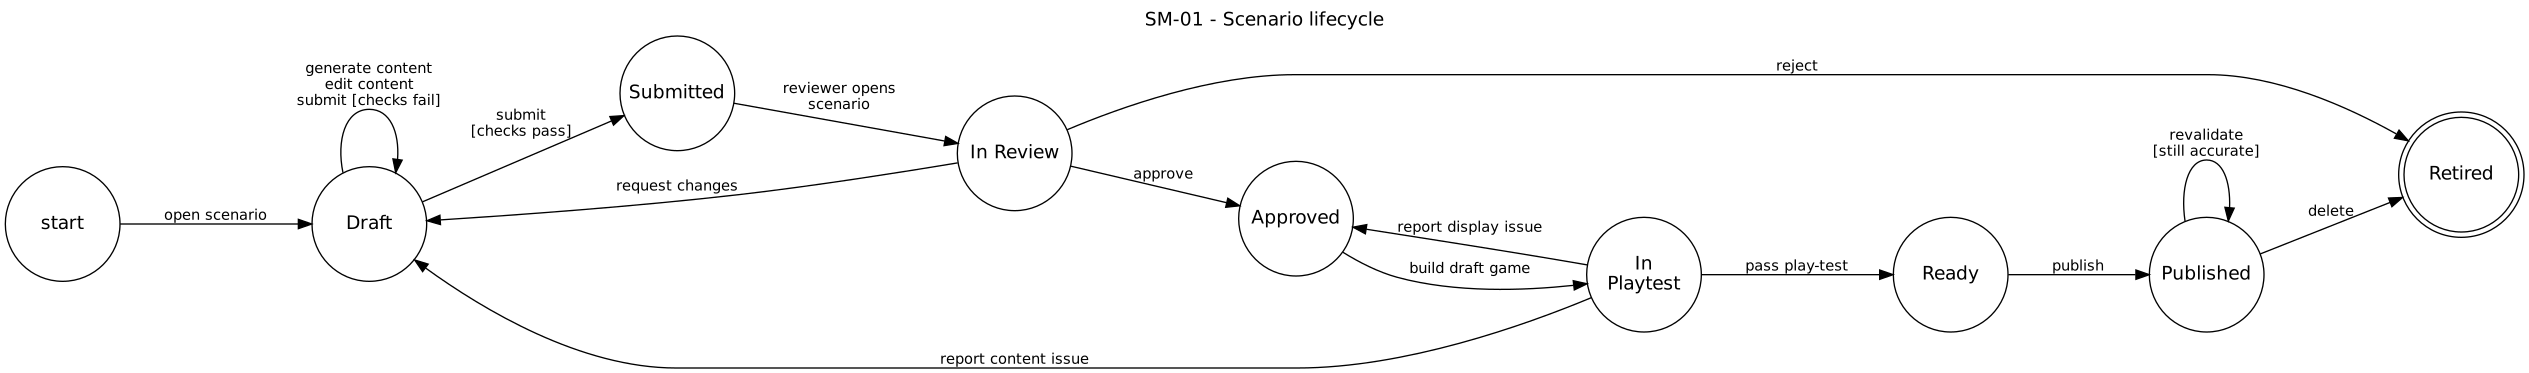
\includegraphics[width=\textwidth,height=0.9\textheight,keepaspectratio]{figures/SM-01_ScenarioLifecycle.png}
\caption{Scenario lifecycle (SM-01)}
\end{figure}

A scenario begins in Draft when the content administrator opens it for a task, and only one scenario per task may be active at a time (FR-33). Draft, Submitted, and In Review belong to the domain experts: the author prepares the content, and a second expert judges it against the review criteria. Approved, In Playtest, and Ready belong to presentation: the content administrator turns the approved content into a game, and the author confirms that the game presents it correctly. Published and Retired are the states explorers can encounter, the first as playable content and the second only in the records of explorers who played it. Retired is final: there is no separate Rejected state, since rejecting or deleting a scenario retires it; a retired scenario cannot be reopened and no longer counts as the active scenario of its task. The table below lists the transitions and the requirement that governs each.

{\small
\begin{longtable}{|>{\raggedright\arraybackslash}p{\dimexpr 0.148\textwidth-2\tabcolsep-\arrayrulewidth\relax}|>{\raggedright\arraybackslash}p{\dimexpr 0.148\textwidth-2\tabcolsep-\arrayrulewidth\relax}|>{\raggedright\arraybackslash}p{\dimexpr 0.528\textwidth-2\tabcolsep-\arrayrulewidth\relax}|>{\raggedright\arraybackslash}p{\dimexpr 0.171\textwidth-2\tabcolsep-\arrayrulewidth\relax}|}
\caption{Transitions of the scenario lifecycle (SM-01).} \\
\hline
\textbf{From} & \textbf{To} & \textbf{Trigger and actor} & \textbf{Requirement} \\ \hline
\endfirsthead
\hline
\textbf{From} & \textbf{To} & \textbf{Trigger and actor} & \textbf{Requirement} \\ \hline
\endhead
(start) & Draft & Open scenario: the content administrator opens a scenario for a task, and the author is notified. A second active scenario for the same task is refused. & FR-33 \\ \hline
Draft & Draft & Generate content, edit content, or submit with failing checks: the author writes the context and generates scenario content with AI, each run kept with its context, model, cost, and check result; a submission that fails the automatic checks leaves the scenario in Draft. & FR-22, FR-23 \\ \hline
Draft & Submitted & Submit: the author submits the scenario after the automatic checks pass; the reviewer assigned with a deadline when the scenario was opened is notified. & FR-23, FR-34 \\ \hline
Submitted & In Review & Reviewer opens scenario: the assigned reviewer, a domain expert other than the author, opens the scenario from the review queue. & FR-25, FR-34 \\ \hline
In Review & Draft & Request changes: the reviewer returns the scenario to its author. & FR-25 \\ \hline
In Review & Approved & Approve: the reviewer approves after answering every review criterion. & FR-25, FR-32 \\ \hline
In Review & Retired & Reject: the reviewer rejects the scenario, which is retired and cannot be reopened. & FR-25 \\ \hline
Approved & In Playtest & Build draft game: the content administrator designs the presentation without changing the content, the draft game is built, and the author is invited to play-test it. & FR-26, FR-35 \\ \hline
In Playtest & Approved & Report display issue: the author finds a presentation problem, and the scenario returns to presentation. & FR-26 \\ \hline
In Playtest & Draft & Report content issue: the author finds a content problem, and the scenario returns to its author and then to review. & FR-26 \\ \hline
In Playtest & Ready & Pass play-test: the author confirms the draft game. Play-test sessions are excluded from explorer data. & FR-26, DR-11 \\ \hline
Ready & Published & Publish: the content administrator publishes the scenario with an effective date and a release note. Publishing is disabled in every other state. & FR-37 \\ \hline
Published & Published & Revalidate, still accurate: a domain expert checks the scenario, on the content administrator's request or after flagged content; it stays published and playable meanwhile, and the result is recorded. & FR-27 \\ \hline
Published & Retired & Delete: the content administrator deletes the scenario, which is retired whether or not explorers have played it; its play history is kept and the task's scenario slot is freed. & FR-38 \\ \hline
\end{longtable}
}

\subsection{Technology Solution}

Each technology in JobQuest is selected by comparing it with its main alternatives against criteria derived from the requirements. Three properties of the requirements drive most choices: a written answer waits several seconds on external models that can fail (NFR-01, NFR-02, NFR-04); scores unlock levels and occupations, so the server must score authoritatively by the same rules the browser uses for immediate feedback (BR-02, BR-11, FR-15); and personal data must be processed and stored in Vietnam (DC-03). The table below sets out nine criteria. The first eight are derived from non-functional requirements and design constraints; the ninth records the project's own constraints, a three-person team and a working prototype written in TypeScript.

{\small
\begin{longtable}{|>{\raggedright\arraybackslash}p{\dimexpr 0.081\textwidth-2\tabcolsep-\arrayrulewidth\relax}|>{\raggedright\arraybackslash}p{\dimexpr 0.505\textwidth-2\tabcolsep-\arrayrulewidth\relax}|>{\raggedright\arraybackslash}p{\dimexpr 0.219\textwidth-2\tabcolsep-\arrayrulewidth\relax}|>{\raggedright\arraybackslash}p{\dimexpr 0.191\textwidth-2\tabcolsep-\arrayrulewidth\relax}|}
\caption{Criteria for comparing technology solutions.} \\
\hline
\textbf{ID} & \textbf{Criterion} & \textbf{Derived from} & \textbf{Applies to} \\ \hline
\endfirsthead
\hline
\textbf{ID} & \textbf{Criterion} & \textbf{Derived from} & \textbf{Applies to} \\ \hline
\endhead
TC1 & Responsiveness while a model works & NFR-01, NFR-02 & Frontend, backend, AI \\ \hline
TC2 & No answer or progress lost on interruption or provider failure & NFR-03, NFR-04 & Frontend, backend, AI \\ \hline
TC3 & Personal data protected and kept in Vietnam & NFR-05, NFR-17, DC-03 & Frontend, backend, AI \\ \hline
TC4 & Usable on mid-range phones and weak networks, without installation & NFR-13, DC-05 & Frontend, backend \\ \hline
TC5 & Accessible, and complete in every supported language & NFR-19, NFR-08 & Frontend \\ \hline
TC6 & One copy of the game rules in browser and server; content kept as versioned data & FR-15, BR-11, NFR-10, NFR-16 & Frontend, backend \\ \hline
TC7 & Model providers replaceable, judge families kept apart & NFR-12, DC-01, DC-02 & Backend, AI \\ \hline
TC8 & Cost and operation sustainable on grant funding & NFR-11, NFR-18 & Backend, AI \\ \hline
TC9 & Feasibility: team skills, maturity, reuse of the working prototype & Project constraint & All \\ \hline
\end{longtable}
}

Ratings use the three symbols of Section 3.3.2, with meanings adapted to technologies: $\bullet$ the option meets the criterion through built-in, documented features; $\ominus$ it meets the criterion with additional work or within a stated limit; $\circ$ it works against the criterion, or meets it only by replacing part of the option. For each component, Sections 5.2.1 to 5.2.3 state what it must do, compare the selected technology with its alternatives on the criteria and requirements that tell them apart, and record the decision; a criterion on which every option rates alike is left out of that component's table. Ratings are the team's assessment from the cited documentation. Where an alternative rates as well as the selected option on the technical criteria, the text says so and states what decided the choice. The selected stack is summarised at the end of Section 5.2.2. Versions are those resolved in the workspace lockfile at the time of writing.

\subsubsection{Frontend}

The frontend serves two populations. Explorers, in twenty of the fifty-three use cases of Section 5.1.2, play on their own phones over weak connections (NFR-13), may use assistive technology (NFR-19), read the interface in Vietnamese (NFR-08), and wait seconds while a model assesses a written answer (NFR-01, NFR-02). Staff, in the other thirty-three, work at desktops in forms, review queues, and tables (FR-21 to FR-43).

Application framework. The frontend must render a game interface with many interacting states --- the occupation map, conversations with characters, the four response forms of FR-10, hints, follow-up questions, and results (FR-05, FR-07, FR-10 to FR-14). It must show provisional feedback on closed formats at once, by the same rules the server applies (FR-15, BR-11), stay responsive while a model works (NFR-01, NFR-02), and load quickly on a mid-range phone without installation (NFR-13, DC-05). Every route except the landing page requires sign-in (FR-01), so no screen needs search indexing.

{\small
\begin{longtable}{|>{\raggedright\arraybackslash}p{\dimexpr 0.171\textwidth-2\tabcolsep-\arrayrulewidth\relax}|>{\raggedright\arraybackslash}p{\dimexpr 0.313\textwidth-2\tabcolsep-\arrayrulewidth\relax}|>{\raggedright\arraybackslash}p{\dimexpr 0.307\textwidth-2\tabcolsep-\arrayrulewidth\relax}|>{\raggedright\arraybackslash}p{\dimexpr 0.205\textwidth-2\tabcolsep-\arrayrulewidth\relax}|}
\caption{Comparison of frontend application frameworks.} \\
\hline
\textbf{Criterion} & \textbf{React 19 + Vite, single-page application (selected)} & \textbf{Next.js, server rendering\cite{r169}} & \textbf{Vue 3 + Vite, single-page application\cite{r170}} \\ \hline
\endfirsthead
\hline
\textbf{Criterion} & \textbf{React 19 + Vite, single-page application (selected)} & \textbf{Next.js, server rendering\cite{r169}} & \textbf{Vue 3 + Vite, single-page application\cite{r170}} \\ \hline
\endhead
Benefit the framework adds & $\circ$ no server rendering, which no screen needs (FR-01) & $\bullet$ server rendering and search indexing, unused behind sign-in & $\circ$ none beyond the selected option \\ \hline
TC3 Personal data & $\bullet$ static files hold no personal data and can sit on a content delivery network & $\ominus$ a rendering server handles personal data and must also be hosted in Vietnam & $\bullet$ static files \\ \hline
TC4 Weak devices and networks & $\bullet$ code split on demand; prototype entry about 195 KB & $\ominus$ less script, but each page waits on a server round trip & $\bullet$ small runtime \\ \hline
TC9 Feasibility & $\bullet$ prototype screens and 3D map already in React; largest ecosystem\cite{r134} & $\ominus$ same components, but server and client boundaries throughout the code & $\circ$ every screen rewritten; React Three Fiber replaced by TresJS\cite{r171} \\ \hline
\end{longtable}
}

\textbf{Decision: React 19 with Vite 8, as a client-rendered single-page application.} React's component model fits an interface of many independent, stateful parts, and it is the most used web framework, by 44.7\% of developers\cite{r134}, so libraries for drag-and-drop ordering, 3D rendering, and accessibility are mature. Running in the browser lets the shared rules package, \textit{game-core}, compute provisional scores without a round trip. React 19's optimistic-update hook shows ``saved, assessing'' the moment an answer is sent\cite{r135}. Vite's production build splits code into chunks loaded on demand\cite{r136}: the prototype's entry was about 195 KB compressed in the build of 18 September 2026, and a budget of 200 KB for the first interactive screen, about one second under the Lighthouse mobile profile\cite{r137}, is checked in continuous integration. Server-side rendering is not used: with every screen behind sign-in it brings no indexing benefit, and it would add a server that renders personal data, whereas static files hold none and can be cached on a content delivery network without affecting DC-03. Vue 3 rates as well on the technical criteria; the choice rests on feasibility, since moving to it would rewrite every screen and the 3D map.

Occupation map. The map must convey the progression metaphor of Section 4.2.1 (FR-05, FR-07), remain operable with a keyboard and a screen reader (NFR-19), and not exclude low-end devices (NFR-13).

{\small
\begin{longtable}{|>{\raggedright\arraybackslash}p{\dimexpr 0.193\textwidth-2\tabcolsep-\arrayrulewidth\relax}|>{\raggedright\arraybackslash}p{\dimexpr 0.344\textwidth-2\tabcolsep-\arrayrulewidth\relax}|>{\raggedright\arraybackslash}p{\dimexpr 0.238\textwidth-2\tabcolsep-\arrayrulewidth\relax}|>{\raggedright\arraybackslash}p{\dimexpr 0.220\textwidth-2\tabcolsep-\arrayrulewidth\relax}|}
\caption{Comparison of occupation map renderings.} \\
\hline
\textbf{Criterion} & \textbf{3D view with an SVG view (selected)} & \textbf{3D view only} & \textbf{2D view only, in SVG} \\ \hline
\endfirsthead
\hline
\textbf{Criterion} & \textbf{3D view with an SVG view (selected)} & \textbf{3D view only} & \textbf{2D view only, in SVG} \\ \hline
\endhead
Progression metaphor (FR-05, FR-07) & $\bullet$ a galaxy of planets to travel between & $\bullet$ same & $\ominus$ a flat map, with a weaker sense of travel \\ \hline
TC4 Weak devices & $\bullet$ SVG view used automatically when WebGL is missing or memory is low & $\circ$ excludes devices without WebGL; GPU work every frame\cite{r139} & $\bullet$ lightest \\ \hline
TC5 Accessibility & $\bullet$ every planet a focusable, named element in the SVG view\cite{r140} & $\circ$ a canvas exposes nothing to a screen reader & $\bullet$ same as the selected option \\ \hline
TC9 Feasibility & $\ominus$ two views drawn from one data model & $\bullet$ exists in the prototype & $\ominus$ a new view; 3D work discarded \\ \hline
\end{longtable}
}

\textbf{Decision: three.js 0.186 through @react-three/fiber 9.7, with an SVG view drawn from the same data.} @react-three/fiber writes the 3D scene as React components that share state with the rest of the interface\cite{r138}. Because a canvas exposes nothing to a screen reader and a 3D scene costs GPU work every frame\cite{r139}, an SVG view, in which each planet is a focusable, named element\cite{r140}, is the accessible equivalent. It can be chosen at any time and is used automatically when WebGL is missing or lost, when reduced motion or data saving is requested, or on low-memory devices. The 3D libraries, about 310 KB compressed, load only when the 3D view opens.

Styling. Styles must add little to the download (NFR-13) and let each occupation carry its own theme without code changes (NFR-10).

{\small
\begin{longtable}{|>{\raggedright\arraybackslash}p{\dimexpr 0.171\textwidth-2\tabcolsep-\arrayrulewidth\relax}|>{\raggedright\arraybackslash}p{\dimexpr 0.290\textwidth-2\tabcolsep-\arrayrulewidth\relax}|>{\raggedright\arraybackslash}p{\dimexpr 0.199\textwidth-2\tabcolsep-\arrayrulewidth\relax}|>{\raggedright\arraybackslash}p{\dimexpr 0.335\textwidth-2\tabcolsep-\arrayrulewidth\relax}|}
\caption{Comparison of styling approaches.} \\
\hline
\textbf{Criterion} & \textbf{Tailwind CSS 4 (selected)} & \textbf{CSS Modules\cite{r172}} & \textbf{CSS-in-JS with a runtime, such as styled-components\cite{r173}} \\ \hline
\endfirsthead
\hline
\textbf{Criterion} & \textbf{Tailwind CSS 4 (selected)} & \textbf{CSS Modules\cite{r172}} & \textbf{CSS-in-JS with a runtime, such as styled-components\cite{r173}} \\ \hline
\endhead
TC4 Download & $\bullet$ only the classes used; no runtime\cite{r141} & $\bullet$ static CSS; no runtime & $\ominus$ styles generated in the browser by script \\ \hline
TC9 Feasibility & $\bullet$ used throughout the prototype & $\ominus$ styles rewritten & $\ominus$ styles rewritten \\ \hline
\end{longtable}
}

\textbf{Decision: Tailwind CSS 4.3.} It generates CSS only for the classes used and has no runtime\cite{r141}; occupation themes are design tokens held as CSS variables and supplied by content data. CSS Modules rate as well technically, and occupation themes as CSS variables work in either; Tailwind is kept because the prototype is already written in it.

Client state. Client state must apply \textit{game-core}'s reducer directly (FR-10, FR-15) and keep unsent turns through a lost connection (NFR-03).

{\small
\begin{longtable}{|>{\raggedright\arraybackslash}p{\dimexpr 0.186\textwidth-2\tabcolsep-\arrayrulewidth\relax}|>{\raggedright\arraybackslash}p{\dimexpr 0.280\textwidth-2\tabcolsep-\arrayrulewidth\relax}|>{\raggedright\arraybackslash}p{\dimexpr 0.209\textwidth-2\tabcolsep-\arrayrulewidth\relax}|>{\raggedright\arraybackslash}p{\dimexpr 0.320\textwidth-2\tabcolsep-\arrayrulewidth\relax}|}
\caption{Comparison of client state libraries.} \\
\hline
\textbf{Criterion} & \textbf{zustand (selected)} & \textbf{Redux Toolkit\cite{r174}} & \textbf{React context with useReducer} \\ \hline
\endfirsthead
\hline
\textbf{Criterion} & \textbf{zustand (selected)} & \textbf{Redux Toolkit\cite{r174}} & \textbf{React context with useReducer} \\ \hline
\endhead
TC2 Unsent turns kept & $\bullet$ persistence middleware\cite{r142} & $\ominus$ needs an added persistence library & $\circ$ written by hand \\ \hline
TC1 Re-rendering & $\bullet$ components subscribe to the part they use & $\bullet$ selectors & $\ominus$ every consumer re-renders on each change \\ \hline
TC4 Download & $\bullet$ very small & $\ominus$ larger & $\bullet$ nothing added \\ \hline
TC9 Feasibility & $\bullet$ used in the prototype & $\ominus$ migration & $\ominus$ persistence and subscriptions written by hand \\ \hline
\end{longtable}
}

\textbf{Decision: zustand 5.0.} A store wraps the reducer, so one dispatch updates both screen and rules state; its persistence middleware keeps unsent turns in browser storage, resent with an idempotency key on reconnection\cite{r142}. It needs no provider tree and adds little to the bundle.

Routing. Routing must keep the 3D map and all staff code out of the explorer's first download (NFR-13), separate explorer and staff areas by role (FR-41), and resume a run on any device (NFR-03).

{\small
\begin{longtable}{|>{\raggedright\arraybackslash}p{\dimexpr 0.239\textwidth-2\tabcolsep-\arrayrulewidth\relax}|>{\raggedright\arraybackslash}p{\dimexpr 0.257\textwidth-2\tabcolsep-\arrayrulewidth\relax}|>{\raggedright\arraybackslash}p{\dimexpr 0.246\textwidth-2\tabcolsep-\arrayrulewidth\relax}|>{\raggedright\arraybackslash}p{\dimexpr 0.252\textwidth-2\tabcolsep-\arrayrulewidth\relax}|}
\caption{Comparison of routing approaches.} \\
\hline
\textbf{Criterion} & \textbf{React Router 7 (selected)} & \textbf{TanStack Router\cite{r175}} & \textbf{Screens switched by application state, without a router} \\ \hline
\endfirsthead
\hline
\textbf{Criterion} & \textbf{React Router 7 (selected)} & \textbf{TanStack Router\cite{r175}} & \textbf{Screens switched by application state, without a router} \\ \hline
\endhead
TC4 Code loaded on demand & $\bullet$ lazy routes & $\bullet$ lazy routes & $\ominus$ split by hand \\ \hline
Areas separated by role (FR-41) & $\bullet$ nested layouts & $\bullet$ nested layouts & $\ominus$ checks written by hand \\ \hline
TC2 Run resumed on any device & $\bullet$ route loaders fetch the run's state\cite{r143} & $\bullet$ route loaders & $\circ$ no address for a run \\ \hline
TC9 Feasibility & $\bullet$ used in the prototype & $\ominus$ migration, in exchange for type-checked routes & $\circ$ \\ \hline
\end{longtable}
}

\textbf{Decision: React Router 7.18.} Routes load on demand, nested layouts separate the areas by role, and route loaders fetch the state of an interrupted run from the server\cite{r143}.

Result delivery. Assessment results must reach the explorer as soon as they are ready (NFR-02, FR-14) over connections that drop (NFR-13). Only the server needs to push; the client submits answers by ordinary requests.

{\small
\begin{longtable}{|>{\raggedright\arraybackslash}p{\dimexpr 0.262\textwidth-2\tabcolsep-\arrayrulewidth\relax}|>{\raggedright\arraybackslash}p{\dimexpr 0.238\textwidth-2\tabcolsep-\arrayrulewidth\relax}|>{\raggedright\arraybackslash}p{\dimexpr 0.254\textwidth-2\tabcolsep-\arrayrulewidth\relax}|>{\raggedright\arraybackslash}p{\dimexpr 0.241\textwidth-2\tabcolsep-\arrayrulewidth\relax}|}
\caption{Comparison of result delivery mechanisms.} \\
\hline
\textbf{Criterion} & \textbf{Server-sent events (selected)} & \textbf{WebSocket\cite{r176}} & \textbf{Polling} \\ \hline
\endfirsthead
\hline
\textbf{Criterion} & \textbf{Server-sent events (selected)} & \textbf{WebSocket\cite{r176}} & \textbf{Polling} \\ \hline
\endhead
TC1 Result shown when ready & $\bullet$ pushed & $\bullet$ pushed & $\ominus$ delayed by the polling interval \\ \hline
TC2, TC4 Dropped connections & $\bullet$ the browser reconnects and resumes from the last event\cite{r144} & $\ominus$ reconnection and replay written by hand & $\bullet$ each request independent \\ \hline
Proxies and load balancers & $\bullet$ plain HTTP & $\ominus$ needs support for upgrading the connection & $\bullet$ plain HTTP \\ \hline
TC8 Load at 5,000 concurrent explorers & $\bullet$ one open stream each & $\bullet$ one connection each & $\circ$ a request every few seconds from each explorer \\ \hline
Direction needed: server to client only & $\bullet$ exactly that & $\ominus$ a two-way channel, half unused & $\ominus$ client asks repeatedly \\ \hline
\end{longtable}
}

\textbf{Decision: server-sent events.} The browser's built-in \textit{EventSource} receives pushed events over plain HTTP, through any proxy, and reconnects by itself\cite{r144}; a bidirectional WebSocket channel is not needed. Polling is kept only as a fallback where a stream cannot be opened (Section 5.3.1).

Staff application. Staff work in review queues, lists, and statistics (FR-21 to FR-43), in dialogs, comboboxes, and grids, where hand-built interfaces most often fail accessibility (NFR-19).

{\small
\begin{longtable}{|>{\raggedright\arraybackslash}p{\dimexpr 0.216\textwidth-2\tabcolsep-\arrayrulewidth\relax}|>{\raggedright\arraybackslash}p{\dimexpr 0.293\textwidth-2\tabcolsep-\arrayrulewidth\relax}|>{\raggedright\arraybackslash}p{\dimexpr 0.261\textwidth-2\tabcolsep-\arrayrulewidth\relax}|>{\raggedright\arraybackslash}p{\dimexpr 0.224\textwidth-2\tabcolsep-\arrayrulewidth\relax}|}
\caption{Comparison of staff interface foundations.} \\
\hline
\textbf{Criterion} & \textbf{React Aria, unstyled primitives (selected)\cite{r146}} & \textbf{MUI component library\cite{r177}} & \textbf{Components built by hand} \\ \hline
\endfirsthead
\hline
\textbf{Criterion} & \textbf{React Aria, unstyled primitives (selected)\cite{r146}} & \textbf{MUI component library\cite{r177}} & \textbf{Components built by hand} \\ \hline
\endhead
TC5 Accessible dialogs, comboboxes, and grids & $\bullet$ accessible behaviour built in & $\bullet$ accessible components & $\circ$ where hand-built interfaces most often fail \\ \hline
Fit with the Tailwind styling & $\bullet$ unstyled, styled with Tailwind & $\ominus$ its own styling system beside Tailwind & $\bullet$ \\ \hline
TC9 Feasibility & $\ominus$ a new library with a small surface & $\ominus$ a new library with a large surface & $\circ$ the most code to write and test \\ \hline
\end{longtable}
}

\textbf{Decision: the same stack, plus TanStack Query and React Aria.} TanStack Query caches and refreshes server data\cite{r145}; React Aria supplies accessible interaction primitives\cite{r146}. The staff application is a separate bundle on the same origin and sign-in screen. For server data, the alternative to TanStack Query is fetching by hand, which repeats loading, caching, and refresh logic on every staff screen.

Localisation. Only Vietnamese is supported in this phase (NFR-08). Interface strings must be complete in every supported language, and adding English later must not require changes to the screens.

{\small
\begin{longtable}{|>{\raggedright\arraybackslash}p{\dimexpr 0.240\textwidth-2\tabcolsep-\arrayrulewidth\relax}|>{\raggedright\arraybackslash}p{\dimexpr 0.348\textwidth-2\tabcolsep-\arrayrulewidth\relax}|>{\raggedright\arraybackslash}p{\dimexpr 0.211\textwidth-2\tabcolsep-\arrayrulewidth\relax}|>{\raggedright\arraybackslash}p{\dimexpr 0.196\textwidth-2\tabcolsep-\arrayrulewidth\relax}|}
\caption{Comparison of localisation approaches.} \\
\hline
\textbf{Criterion} & \textbf{Typed message table with the Intl API (selected)} & \textbf{i18next\cite{r178}} & \textbf{Strings written in components} \\ \hline
\endfirsthead
\hline
\textbf{Criterion} & \textbf{Typed message table with the Intl API (selected)} & \textbf{i18next\cite{r178}} & \textbf{Strings written in components} \\ \hline
\endhead
TC5 Missing strings caught & $\bullet$ an unknown key fails compilation; a test checks completeness & $\ominus$ type checking needs extra setup & $\circ$ not detectable \\ \hline
English added later as data & $\bullet$ & $\bullet$ & $\circ$ every screen edited \\ \hline
TC4 Download & $\bullet$ no library & $\ominus$ a library added & $\bullet$ \\ \hline
TC9 Feasibility & $\bullet$ used in the prototype & $\ominus$ migration & $\circ$ \\ \hline
\end{longtable}
}

\textbf{Decision: a typed message table with the standard \textit{Intl} API.} An unknown key fails compilation and a test fails a missing translation; plurals, dates, and numbers are formatted by \textit{Intl}\cite{r147}; content fields carry a locale, so a second language is added as data. Generated text is inserted as text, which React escapes, so model output cannot inject markup (NFR-17)\cite{r148}.

\subsubsection{Backend}

The backend carries five kinds of work: short requests for navigation, records, and staff edits; durable recording of every turn as it happens (NFR-03); assessment and follow-up generation, which wait seconds on external models and occasionally fail (NFR-01, NFR-02, NFR-04); authoritative scoring (BR-02, BR-11); and a governed content lifecycle with logged transitions (NFR-16).

Application framework. Most backend time is spent waiting --- on models, on the database, on open result streams --- and at Stage 4 about five thousand explorers are connected at once (Section 5.3.1). The framework must also give the modular structure of Section 5.3.1 clear module boundaries, check occupation-scoped roles on every request (FR-40, FR-41), integrate a job queue and server-sent events, and score by the same rules as the browser (FR-15, BR-11).

{\small
\begin{longtable}{|>{\raggedright\arraybackslash}p{\dimexpr 0.213\textwidth-2\tabcolsep-\arrayrulewidth\relax}|>{\raggedright\arraybackslash}p{\dimexpr 0.287\textwidth-2\tabcolsep-\arrayrulewidth\relax}|>{\raggedright\arraybackslash}p{\dimexpr 0.289\textwidth-2\tabcolsep-\arrayrulewidth\relax}|>{\raggedright\arraybackslash}p{\dimexpr 0.207\textwidth-2\tabcolsep-\arrayrulewidth\relax}|}
\caption{Comparison of backend frameworks.} \\
\hline
\textbf{Criterion} & \textbf{NestJS 11 on Node.js (selected)} & \textbf{Spring Boot, Java\cite{r179}} & \textbf{FastAPI, Python\cite{r181}} \\ \hline
\endfirsthead
\hline
\textbf{Criterion} & \textbf{NestJS 11 on Node.js (selected)} & \textbf{Spring Boot, Java\cite{r179}} & \textbf{FastAPI, Python\cite{r181}} \\ \hline
\endhead
TC1 Waiting on models and open streams & $\bullet$ event loop; a waiting request costs memory, not a thread & $\ominus$ a thread per request by default; virtual threads\cite{r180} or a reactive stack for thousands of streams & $\bullet$ asynchronous by design \\ \hline
TC6 Same rules as the browser & $\bullet$ imports game-core & $\circ$ rules rewritten in Java; two copies to keep equal & $\circ$ rules rewritten in Python \\ \hline
Modules, role guards, queue and stream integration & $\bullet$ first-party\cite{r149} & $\bullet$ mature equivalents & $\ominus$ assembled from separate libraries \\ \hline
Access to AI libraries & $\ominus$ provider SDKs in TypeScript; statistics offline in Python & $\ominus$ fewer AI libraries & $\bullet$ the Python ecosystem \\ \hline
TC9 Feasibility & $\bullet$ the prototype API is NestJS; the team writes TypeScript & $\ominus$ a new language and framework & $\ominus$ a new language for the API \\ \hline
\end{longtable}
}

\textbf{Decision: NestJS 11.1 on Node.js, in TypeScript.} Node.js serves I/O on an event loop, so a waiting request or open stream costs memory rather than a thread. NestJS modules and dependency injection give each bounded context its own module; guards enforce occupation-scoped roles; interceptors write the activity log; and first-party integrations provide BullMQ queues and server-sent events\cite{r149}. Dependency injection also binds the model port to the provider adapter named in configuration (DC-02, NFR-12)\cite{r150}. The server imports the same \textit{game-core} package as the browser and recomputes every score from stored events. Models are called over HTTP and run nowhere in the process, so the request path needs no Python; the statistics for evaluating RP-1 and RP-2 run offline in Python scripts. Long computation, which would block an event loop, runs in worker processes. FastAPI's advantage, the Python AI ecosystem, is not needed on the request path, because models are called over HTTP; it would cost a second copy of the game rules.

Database. Much of the data is relational, with rules that span records: a reviewer is never the author (FR-25), one active scenario per task (FR-33), exactly one content administrator per occupation (FR-40), and the replay cap (BR-11). Publication and its log must be atomic, and published content immutable (NFR-16); scenario content is nested documents (NFR-10, NFR-15); statistics are shown only above a population threshold (NFR-06, FR-19, FR-39); and the store must be hostable in Vietnam (DC-03).

{\small
\begin{longtable}{|>{\raggedright\arraybackslash}p{\dimexpr 0.265\textwidth-2\tabcolsep-\arrayrulewidth\relax}|>{\raggedright\arraybackslash}p{\dimexpr 0.244\textwidth-2\tabcolsep-\arrayrulewidth\relax}|>{\raggedright\arraybackslash}p{\dimexpr 0.204\textwidth-2\tabcolsep-\arrayrulewidth\relax}|>{\raggedright\arraybackslash}p{\dimexpr 0.283\textwidth-2\tabcolsep-\arrayrulewidth\relax}|}
\caption{Comparison of databases.} \\
\hline
\textbf{Criterion} & \textbf{PostgreSQL with Prisma (selected)} & \textbf{MongoDB\cite{r182}} & \textbf{MySQL 8\cite{r183}} \\ \hline
\endfirsthead
\hline
\textbf{Criterion} & \textbf{PostgreSQL with Prisma (selected)} & \textbf{MongoDB\cite{r182}} & \textbf{MySQL 8\cite{r183}} \\ \hline
\endhead
Rules across records enforced by the database (FR-25, FR-33, FR-40) & $\bullet$ foreign keys, checks, partial unique indexes\cite{r151} & $\ominus$ no foreign keys; rules kept in application code & $\ominus$ foreign keys and checks; no partial indexes, functional indexes as a workaround \\ \hline
Publication and its log in one transaction (NFR-16) & $\bullet$ transactions & $\bullet$ multi-document transactions\cite{r182} & $\bullet$ transactions \\ \hline
Nested scenario content (NFR-10, NFR-15) & $\bullet$ indexable jsonb\cite{r152} & $\bullet$ native documents & $\ominus$ JSON type, indexed through functional indexes \\ \hline
Statistics above a threshold (NFR-06) & $\bullet$ window functions and materialised views & $\ominus$ aggregation pipeline & $\ominus$ window functions; no materialised views \\ \hline
TC9 Feasibility & $\bullet$ the prototype schema, 19 tables & $\circ$ data re-modelled & $\ominus$ supported by Prisma; migrations rewritten \\ \hline
\end{longtable}
}

\textbf{Decision: PostgreSQL, accessed through Prisma ORM 7.10.} Foreign keys, check constraints, partial unique indexes, and transactions enforce the cross-record rules in the database itself --- ``one active scenario per task'' is a single partial index\cite{r151}. A transition and its log entry share one transaction, and a trigger refuses updates to published releases. Content is stored in \textit{jsonb} columns\cite{r152}, validated by \textit{game-core}'s schemas on write and read. Thresholded statistics are SQL grouping, window functions, and materialised views. PostgreSQL is open source, offered by every cloud provider, and the most used database, at 55.6\%\cite{r134}. Prisma generates a typed client from the schema and, from version 7, runs over the standard \textit{pg} driver\cite{r153}; partial indexes, checks, and triggers, which Prisma does not express, live in SQL migrations and are tested against the database.

Job queue and messaging. Model work must survive failures, be retried, and be listed for re-run when it fails (NFR-04, FR-43); it must respect each provider's rate limits and serve live play first --- narration and follow-ups for an explorer in a scenario before background scoring, and both before authoring work (NFR-01, NFR-11); results must reach the API replica holding the explorer's stream (NFR-02); and each session's model cost must be counted atomically (NFR-11).

{\small
\begin{longtable}{|>{\raggedright\arraybackslash}p{\dimexpr 0.273\textwidth-2\tabcolsep-\arrayrulewidth\relax}|>{\raggedright\arraybackslash}p{\dimexpr 0.248\textwidth-2\tabcolsep-\arrayrulewidth\relax}|>{\raggedright\arraybackslash}p{\dimexpr 0.224\textwidth-2\tabcolsep-\arrayrulewidth\relax}|>{\raggedright\arraybackslash}p{\dimexpr 0.250\textwidth-2\tabcolsep-\arrayrulewidth\relax}|}
\caption{Comparison of job queues.} \\
\hline
\textbf{Criterion} & \textbf{Redis with BullMQ (selected)} & \textbf{RabbitMQ\cite{r184}} & \textbf{pg-boss on PostgreSQL\cite{r185}} \\ \hline
\endfirsthead
\hline
\textbf{Criterion} & \textbf{Redis with BullMQ (selected)} & \textbf{RabbitMQ\cite{r184}} & \textbf{pg-boss on PostgreSQL\cite{r185}} \\ \hline
\endhead
Retries with backoff, priorities, failed jobs listed (NFR-04, FR-43) & $\bullet$ built in\cite{r154} & $\ominus$ priorities and dead-letter queues built in; delayed retries configured by hand & $\bullet$ retries with backoff, priority and dead-letter queues \\ \hline
Rate limits per provider (NFR-11) & $\bullet$ per-queue limiter & $\ominus$ written by hand & $\bullet$ queue policies \\ \hline
Results to every API replica (NFR-02) & $\bullet$ publish--subscribe & $\bullet$ exchanges & $\ominus$ publish--subscribe through the database \\ \hline
Atomic cost counter per session (NFR-11) & $\bullet$ atomic counters & $\circ$ needs a separate store & $\bullet$ transactional update \\ \hline
Load on the system of record at Stage 4 & $\bullet$ none; Redis holds nothing that cannot be rebuilt & $\bullet$ none & $\ominus$ about one hundred jobs per second written to PostgreSQL \\ \hline
TC8 Services to operate & $\ominus$ one more service & $\ominus$ one more service, plus a store for counters & $\bullet$ none added \\ \hline
TC9 Feasibility & $\bullet$ first-party NestJS integration\cite{r149}; declared in the prototype & $\ominus$ new & $\ominus$ new \\ \hline
\end{longtable}
}

\textbf{Decision: Redis with BullMQ 6.3.} BullMQ provides persisted jobs, retries with exponential backoff, job priorities, per-queue rate limiting, and a set of failed jobs for re-run\cite{r154}; Redis's publish--subscribe carries results to every API replica, and its atomic counters meter the session budget. Redis holds nothing that cannot be rebuilt from PostgreSQL, and a scheduled reconciliation re-queues any stored answer without a result, so losing Redis loses no answer. pg-boss is the closest alternative and would avoid running Redis during the pilots; BullMQ is chosen to keep queue traffic off the system of record at national scale and for its first-party NestJS integration.

Authentication. The platform must register, sign in, recover, and delete accounts (FR-01, FR-02); hash passwords, protect sessions, and end idle ones (NFR-17); scope roles to occupations (FR-41); and keep identity data in Vietnam (DC-03).

{\small
\begin{longtable}{|>{\raggedright\arraybackslash}p{\dimexpr 0.182\textwidth-2\tabcolsep-\arrayrulewidth\relax}|>{\raggedright\arraybackslash}p{\dimexpr 0.326\textwidth-2\tabcolsep-\arrayrulewidth\relax}|>{\raggedright\arraybackslash}p{\dimexpr 0.280\textwidth-2\tabcolsep-\arrayrulewidth\relax}|>{\raggedright\arraybackslash}p{\dimexpr 0.208\textwidth-2\tabcolsep-\arrayrulewidth\relax}|}
\caption{Comparison of authentication solutions.} \\
\hline
\textbf{Criterion} & \textbf{The platform's own module (selected)} & \textbf{Keycloak, self-hosted\cite{r186}} & \textbf{Managed service, such as Firebase Authentication\cite{r187}} \\ \hline
\endfirsthead
\hline
\textbf{Criterion} & \textbf{The platform's own module (selected)} & \textbf{Keycloak, self-hosted\cite{r186}} & \textbf{Managed service, such as Firebase Authentication\cite{r187}} \\ \hline
\endhead
TC3 Identity data in Vietnam & $\bullet$ in the platform's database in Vietnam & $\bullet$ hosted in Vietnam & $\circ$ held by the provider abroad \\ \hline
Roles scoped to occupations (FR-41) & $\bullet$ in the application & $\ominus$ roles in Keycloak; occupation scope still checked in the application & $\ominus$ same \\ \hline
Security baseline (NFR-17) & $\ominus$ to be completed to ASVS level 2\cite{r157}: reset, idle expiry, second factor for staff & $\bullet$ reset, sessions, second factor built in & $\bullet$ built in \\ \hline
TC8 Operation & $\bullet$ no extra service & $\circ$ a separate identity server to run, upgrade, and secure & $\ominus$ no server; one vendor for every account \\ \hline
TC9 Feasibility & $\bullet$ registration, Google sign-in, rotating refresh tokens exist in the prototype & $\ominus$ migration & $\ominus$ migration \\ \hline
\end{longtable}
}

\textbf{Decision: the platform's own module --- argon2id, JWT access and refresh tokens in httpOnly cookies, and optional Google sign-in.} Passwords are hashed with argon2id\cite{r155}; a fifteen-minute access token and a rotating refresh token with reuse detection\cite{r156} live in httpOnly, SameSite cookies that scripts cannot read; Google ID tokens are verified with google-auth-library. Accounts stay in the platform's database in Vietnam, which an external identity service would hold abroad, and occupation-scoped authorisation must live in the application whichever service is used. The module is completed against ASVS 5.0 level 2\cite{r157}: single-use, short-lived reset tokens; an inactivity limit; account status checked on every refresh and staff request; rate limiting of sign-in; and a second factor for staff. The remaining risk is the security work that Keycloak would supply ready-made, which is why the module is held to ASVS level 2 and tested against it.

Validation and code organisation. Every input and every model output must be checked against a schema (NFR-17, FR-11), and one copy of the rules and contracts must serve both applications, the API, and the worker (FR-15).

{\small
\begin{longtable}{|>{\raggedright\arraybackslash}p{\dimexpr 0.260\textwidth-2\tabcolsep-\arrayrulewidth\relax}|>{\raggedright\arraybackslash}p{\dimexpr 0.346\textwidth-2\tabcolsep-\arrayrulewidth\relax}|>{\raggedright\arraybackslash}p{\dimexpr 0.223\textwidth-2\tabcolsep-\arrayrulewidth\relax}|>{\raggedright\arraybackslash}p{\dimexpr 0.166\textwidth-2\tabcolsep-\arrayrulewidth\relax}|}
\caption{Comparison of validation libraries.} \\
\hline
\textbf{Criterion} & \textbf{Zod 4 (selected)} & \textbf{class-validator\cite{r188}} & \textbf{JSON Schema with Ajv\cite{r189}} \\ \hline
\endfirsthead
\hline
\textbf{Criterion} & \textbf{Zod 4 (selected)} & \textbf{class-validator\cite{r188}} & \textbf{JSON Schema with Ajv\cite{r189}} \\ \hline
\endhead
TC6 One schema for browser, API, and worker & $\bullet$ plain TypeScript that runs anywhere & $\ominus$ decorated classes, suited to the server & $\bullet$ language-neutral \\ \hline
Schemas for model output (FR-11) & $\bullet$ exported as JSON Schema for providers' structured output\cite{r190} & $\ominus$ needs another library to export & $\bullet$ native \\ \hline
Types in the code & $\bullet$ inferred from the schema & $\ominus$ classes double as types & $\ominus$ types generated separately \\ \hline
Read by the offline Python harness & $\bullet$ through the JSON Schema export & $\circ$ & $\bullet$ \\ \hline
TC9 Feasibility & $\bullet$ the prototype validates game data with Zod & $\ominus$ & $\ominus$ \\ \hline
\end{longtable}
}

{\small
\begin{longtable}{|>{\raggedright\arraybackslash}p{\dimexpr 0.286\textwidth-2\tabcolsep-\arrayrulewidth\relax}|>{\raggedright\arraybackslash}p{\dimexpr 0.253\textwidth-2\tabcolsep-\arrayrulewidth\relax}|>{\raggedright\arraybackslash}p{\dimexpr 0.277\textwidth-2\tabcolsep-\arrayrulewidth\relax}|>{\raggedright\arraybackslash}p{\dimexpr 0.179\textwidth-2\tabcolsep-\arrayrulewidth\relax}|}
\caption{Comparison of code organisation.} \\
\hline
\textbf{Criterion} & \textbf{Nx monorepo (selected)} & \textbf{Separate repositories, shared package published} & \textbf{pnpm workspaces alone} \\ \hline
\endfirsthead
\hline
\textbf{Criterion} & \textbf{Nx monorepo (selected)} & \textbf{Separate repositories, shared package published} & \textbf{pnpm workspaces alone} \\ \hline
\endhead
TC6 One copy of game-core and the schemas & $\bullet$ & $\ominus$ versions published and kept in step & $\bullet$ \\ \hline
TC4 Staff code kept out of the explorer's download & $\bullet$ module-boundary rules enforced\cite{r158} & $\bullet$ separated by construction & $\ominus$ not enforced \\ \hline
Only what changed is built and tested & $\bullet$ affected tasks and caching\cite{r158} & $\ominus$ per repository & $\ominus$ by hand \\ \hline
TC9 Feasibility & $\bullet$ the prototype is an Nx workspace & $\circ$ repository split & $\ominus$ Nx already runs on pnpm workspaces \\ \hline
\end{longtable}
}

\textbf{Decision: Zod 4.6 schemas in an Nx 23.1 monorepo.} Zod schemas, shared by API, clients, and the rule checks, validate requests, content documents, and model output --- scores within rubric anchors, quotations verbatim. Nx keeps \textit{game-core} and the schemas in one repository, enforces module boundaries so staff code never enters the explorer's bundle (NFR-13), and builds and tests only what a change affects\cite{r158}.

Packaging and hosting. Personal data must be stored in Vietnam (DC-03, NFR-05) --- Decree 53/2022 further requires domestic online-service enterprises to store users' data in Vietnam, applicability to be confirmed (Section 4.1.4)\cite{r159,r160} --- and the platform must stay available (NFR-18) while growing from a university pilot to a national service.

{\small
\begin{longtable}{|>{\raggedright\arraybackslash}p{\dimexpr 0.167\textwidth-2\tabcolsep-\arrayrulewidth\relax}|>{\raggedright\arraybackslash}p{\dimexpr 0.293\textwidth-2\tabcolsep-\arrayrulewidth\relax}|>{\raggedright\arraybackslash}p{\dimexpr 0.197\textwidth-2\tabcolsep-\arrayrulewidth\relax}|>{\raggedright\arraybackslash}p{\dimexpr 0.338\textwidth-2\tabcolsep-\arrayrulewidth\relax}|}
\caption{Comparison of hosting options.} \\
\hline
\textbf{Criterion} & \textbf{Containers hosted in Vietnam (selected)} & \textbf{Cloud region abroad, such as Singapore} & \textbf{Serverless functions} \\ \hline
\endfirsthead
\hline
\textbf{Criterion} & \textbf{Containers hosted in Vietnam (selected)} & \textbf{Cloud region abroad, such as Singapore} & \textbf{Serverless functions} \\ \hline
\endhead
TC3 Data in Vietnam & $\bullet$ system of record in Vietnam; only de-identified text leaves & $\circ$ every account becomes a cross-border transfer\cite{r99} & $\ominus$ only where the platform has a region in Vietnam \\ \hline
TC1 Request path & $\bullet$ long-running processes & $\bullet$ long-running processes & $\ominus$ cold starts on the request path (Section 5.3.1) \\ \hline
Open streams and queue workers & $\bullet$ & $\bullet$ & $\circ$ short-lived functions; streams and workers need other services \\ \hline
TC8 Operation & $\ominus$ the team runs containers; a university server at Stage 1 & $\ominus$ same & $\bullet$ scaling managed by the platform \\ \hline
Moving host & $\bullet$ portable services only & $\bullet$ & $\circ$ tied to one platform's interfaces \\ \hline
\end{longtable}
}

\textbf{Decision: Docker containers, hosted in Vietnam.} One image runs as API or worker, with rolling deployment and health checks, and the platform depends only on portable services --- PostgreSQL, Redis, and S3-compatible storage --- so moving host is a change of configuration. The system of record runs on university infrastructure for the Stage 1 pilot and on a cloud provider in Vietnam from Stage 2\cite{r161}; an international region such as Singapore would make every account a cross-border transfer\cite{r99}. Only de-identified text leaves the country, through the model gateway. International providers adding capacity in Vietnam, such as the AWS Hanoi Local Zone, whose control plane remains in Singapore\cite{r162}, are reassessed with the legal office before Stage 2.

\subsubsection{AI algorithms, technologies, and models}

The project does not design, train, or fine-tune a model. It composes existing language models, under rules and expert oversight, so that the problem of Section 4.2.2 is solved: occupational scenarios that stay faithful to expert content (RP-1) and free-text answers scored in agreement with experts (RP-2). The choices that shape that composition are compared here; how the selected parts work together is designed in Section 5.3.6, and how well they work is evaluated in Section 7.3.

Where AI works. AI is used at five steps, three while content is authored and two during play. AI drafts, connects, scores, and filters; domain experts decide occupational content, scoring keys, and publication; deterministic rules, not models, check what models produce while an explorer is waiting.

{\small
\begin{longtable}{|>{\raggedright\arraybackslash}p{\dimexpr 0.092\textwidth-2\tabcolsep-\arrayrulewidth\relax}|>{\raggedright\arraybackslash}p{\dimexpr 0.471\textwidth-2\tabcolsep-\arrayrulewidth\relax}|>{\raggedright\arraybackslash}p{\dimexpr 0.432\textwidth-2\tabcolsep-\arrayrulewidth\relax}|}
\caption{The five AI components and the human decision attached to each.} \\
\hline
\textbf{Step} & \textbf{What AI does} & \textbf{What a person decides} \\ \hline
\endfirsthead
\hline
\textbf{Step} & \textbf{What AI does} & \textbf{What a person decides} \\ \hline
\endhead
AI-1 & Interviews the domain expert to collect what a scenario seed needs & The expert confirms the record \\ \hline
AI-2 & Turns the expert's input into a structured game seed, with the content administrator & The expert sets every scoring key and rubric anchor, and approves the seed \\ \hline
AI-3 & Runs test playthroughs and picks the cases the expert must see & The expert rules on them and approves publication \\ \hline
AI-4 & Writes connecting narration, follow-up questions, and feedback notes during play & Nobody at run time; the engine and rules constrain it, and the expert writes the default follow-up \\ \hline
AI-5 & Grades each answer against the rubric & The expert reviews flagged cases \\ \hline
\end{longtable}
}

AI-1, interviewing the domain expert. A language model asks and probes to collect what a seed needs: incidents, what a good and a poor response look like, and the facts of the situation. Each expert is interviewed separately, and the merged content marks where experts agree and where they differ. The interview is constrained by a human-written topic guide based on the critical incident technique\cite{r26} and on development practice for situational judgment tests\cite{r27}; the model probes inside each topic only. A tracker lists the seed fields still missing, the expert is shown a summary and confirms it, and every turn is stored verbatim so that each seed field links to the turn it came from. That a language model can hold an interview to a guide is supported by 766 AI-led interviews in which 94.8\% to 99.8\% of questions were open-ended, 95.7\% to 99.6\% neutral, and 0.1\% to 0.4\% hallucinated\cite{r114}.

AI-2, drafting the game seed. The model helps the content administrator turn the experts' answers into a structured seed: context, characters, situations, canon events, and the scoring frame. Drafts are written from the expert's own words, the domain expert sets every scoring key and every rubric anchor, and a seed passes automatic structure checks and then the expert's approval before any player sees it. Experts own keys and rubrics because, when GPT-4 drafted 210 examination questions, specialists required revision of 15\% and judged 0.5\% false\cite{r115}. The seed follows evidence-centered design: what is measured, which behaviour is evidence for it, and which situation elicits that behaviour\cite{r20,r116}. This is the first of four checkpoints for generated content: structure is checked by machine and content is approved by the expert.

AI-3, helping the expert test before publishing. A volunteer expert with about seven hours cannot read every free-text answer. AI-3 runs AI-4 and AI-5 on test playthroughs, from experts, testers, and simulated answers, and ranks the cases that need the expert: cases where the three judges differ by more than one level, generated turns that broke a run-time rule, and a blind random sample of cases that were not flagged. The expert decides, and can refine a rubric anchor during review, so rubrics are versioned. The random sample is required because confidence signals from a language-model grader separate right from wrong grades only weakly, with an area under the curve of 0.57 to 0.64\cite{r117}, so flagged cases alone can hide errors; if n audited cases show no error, the error rate is at most about 3/n at 95\% confidence\cite{r118}. Simulated players find relative problems only: persona-prompted models answered with near-perfect, uniform accuracy, unlike 2,359 real students\cite{r119}, so real test plays are needed as well. The run-time checks of AI-4 are to be tested on scripted player turns in four classes (on-script, off-script, adversarial, and rubric-fishing), reporting the violation rate per class; this test set is not yet built. This is the second checkpoint, and the expert-scored test plays are also the validation data for the judge. In the present phase there are no experts or real players: the team stands in for both and the advisor checks a sample, so results show that the machinery works, not agreement with experts.

AI-4, narrating during play. The game engine, not the model, controls the order of canon events. Canon content is shown verbatim from the seed; a situation may have several approved canon variants chosen at random, and the log records which variant was served. The model writes only the connecting narration, the follow-up questions that fit the player's free-text answer, and a hidden feedback note after each activity. A follow-up is decided only after the answer it follows has been graded (AI-5); a follow-up that fails the run-time checks is replaced by the expert's default follow-up, and a feedback note that fails them is redrafted, since feedback has no expert default. The whole seed is placed in the prompt, without retrieval or fine-tuning, and the rubric and scoring keys are not in the prompt. Run-time checks are rules, not another model call, so checking adds no waiting time: numbers and names must come from the seed or from the player's own text, and the engine counts follow-ups. A model from a different family reviews the logs afterwards. Holding authored structure outside free generation is the established approach in interactive narrative\cite{r120}, and when the source fits in the prompt, long-context prompting outperformed retrieval on average\cite{r121}. These are the third checkpoint (rules at run time) and the fourth (log review afterwards).

AI-5, grading each answer. The scoring model is separate from the narrating model (DC-01). There is no reference answer: answers are free text, and the judge scores each rubric criterion by how far the answer meets the behaviour described for each level. Each judge is called once per answer, follow-up answers included, with at most three criteria in a call; the call is made as soon as the answer is submitted, and the follow-up is decided only once the grade is known (FR-11, FR-12). For each criterion the judge returns a verbatim quote from the player, then the rationale, then the level, and the quote must be a substring of what the player typed. A panel of three judges from three model families grades each answer and the median is the score; cases where judges differ by more than one level go to the expert through AI-3, and if a judge is unavailable, the system switches to the other tier of the same family, so that the panel keeps three families (DC-01); if neither tier is available, the system reports an error and keeps the answers (NFR-04). One call for all criteria was not chosen because batching several rubric checks into one call trades accuracy for cost, with a large loss when the evidence is spread over a long trajectory\cite{r122}. A panel was chosen because a five-judge vote matched the best single judge, with a Pearson correlation with humans of 0.627 against 0.623\cite{r123}, so a panel reaches the best judge's level without knowing in advance which judge that is. The design does not claim that a panel is more accurate than a single judge.

Holding generation to expert content. The narrator (AI-4) must not invent occupational facts (RP-1, NFR-15), must change when an expert revises a seed (BR-14), and must not tie the platform to one provider (TC7).

{\small
\begin{longtable}{|>{\raggedright\arraybackslash}p{\dimexpr 0.199\textwidth-2\tabcolsep-\arrayrulewidth\relax}|>{\raggedright\arraybackslash}p{\dimexpr 0.314\textwidth-2\tabcolsep-\arrayrulewidth\relax}|>{\raggedright\arraybackslash}p{\dimexpr 0.200\textwidth-2\tabcolsep-\arrayrulewidth\relax}|>{\raggedright\arraybackslash}p{\dimexpr 0.281\textwidth-2\tabcolsep-\arrayrulewidth\relax}|}
\caption{Comparison of ways to hold generation to expert content.} \\
\hline
\textbf{Criterion} & \textbf{Whole seed in the prompt, structured output, rule checks (selected)} & \textbf{Retrieval over the expert material} & \textbf{Fine-tuning a model on expert scenarios} \\ \hline
\endfirsthead
\hline
\textbf{Criterion} & \textbf{Whole seed in the prompt, structured output, rule checks (selected)} & \textbf{Retrieval over the expert material} & \textbf{Fine-tuning a model on expert scenarios} \\ \hline
\endhead
Fidelity to expert content (RP-1, NFR-15) & $\bullet$ the whole seed in context; canon shown verbatim; names and numbers checked\cite{r120,r121} & $\ominus$ retrieval can miss a required fact & $\circ$ facts held in weights; required facts not guaranteed \\ \hline
Data needed in this phase & $\bullet$ one approved seed & $\bullet$ the same material, indexed & $\circ$ many expert-written scenarios, which do not yet exist (Section 4.2.1) \\ \hline
Seed revised by an expert (BR-14) & $\bullet$ takes effect at once & $\bullet$ re-indexed & $\circ$ model retrained \\ \hline
TC7 Provider replaceable & $\bullet$ any model with a long enough context & $\bullet$ & $\circ$ tied to the tuned model \\ \hline
TC8 Cost per call & $\ominus$ long prompts, reduced by prompt caching & $\ominus$ shorter prompts, plus an index to run & $\ominus$ cheaper calls, plus training \\ \hline
\end{longtable}
}

\textbf{Decision: the whole seed in the prompt, with structured output and rule checks.} A seed fits in the context of every candidate model, so retrieval adds a way to miss a fact without saving anything that matters, and fine-tuning needs data the project will not have before Stage B. When the source fits in the prompt, long-context prompting outperformed retrieval on average\cite{r121}; holding authored structure outside free generation is the established approach in interactive narrative\cite{r120}.

Checking generated text while the explorer waits. Every narration and follow-up must be checked before it is shown (NFR-15), within the five seconds of NFR-01.

{\small
\begin{longtable}{|>{\raggedright\arraybackslash}p{\dimexpr 0.228\textwidth-2\tabcolsep-\arrayrulewidth\relax}|>{\raggedright\arraybackslash}p{\dimexpr 0.355\textwidth-2\tabcolsep-\arrayrulewidth\relax}|>{\raggedright\arraybackslash}p{\dimexpr 0.231\textwidth-2\tabcolsep-\arrayrulewidth\relax}|>{\raggedright\arraybackslash}p{\dimexpr 0.182\textwidth-2\tabcolsep-\arrayrulewidth\relax}|}
\caption{Comparison of ways to check generated text at run time.} \\
\hline
\textbf{Criterion} & \textbf{Deterministic rules at run time, log review by another family afterwards (selected)} & \textbf{A guard model on every turn\cite{r199}} & \textbf{Prompt instructions only} \\ \hline
\endfirsthead
\hline
\textbf{Criterion} & \textbf{Deterministic rules at run time, log review by another family afterwards (selected)} & \textbf{A guard model on every turn\cite{r199}} & \textbf{Prompt instructions only} \\ \hline
\endhead
NFR-01 Time added while waiting & $\bullet$ milliseconds & $\circ$ a second model call on every turn & $\bullet$ none \\ \hline
NFR-15 Invented names and numbers & $\bullet$ every name and number must occur in the seed or the explorer's text & $\ominus$ judged by a model, with its own errors & $\circ$ not checked \\ \hline
Follow-up limits and leaked rubric text & $\bullet$ counted and matched by the engine & $\ominus$ & $\circ$ \\ \hline
Tone, plausibility, subtle drift & $\ominus$ caught afterwards by the log review & $\bullet$ caught before display & $\circ$ \\ \hline
TC6 One rule set & $\bullet$ the same checks in \textit{game-core}, client and server & $\circ$ a separate model to configure & $\circ$ \\ \hline
\end{longtable}
}

\textbf{Decision: deterministic rules at run time, and a model of another family reviewing the logs afterwards.} The rules catch exactly the failures that matter most to fidelity, invented names and numbers, and they cost no waiting time; what rules cannot judge, tone and plausibility, is left to a review that does not delay the explorer. A text that fails the rules is regenerated a bounded number of times and then handled as a model failure (Section 5.3.6).

Scoring free-text answers. The scorer (AI-5) must agree with experts (RP-2, NFR-14) without reference answers, be independent of the narrator (DC-01), and tell the expert which cases to review (AI-3).

{\small
\begin{longtable}{|>{\raggedright\arraybackslash}p{\dimexpr 0.199\textwidth-2\tabcolsep-\arrayrulewidth\relax}|>{\raggedright\arraybackslash}p{\dimexpr 0.317\textwidth-2\tabcolsep-\arrayrulewidth\relax}|>{\raggedright\arraybackslash}p{\dimexpr 0.219\textwidth-2\tabcolsep-\arrayrulewidth\relax}|>{\raggedright\arraybackslash}p{\dimexpr 0.260\textwidth-2\tabcolsep-\arrayrulewidth\relax}|}
\caption{Comparison of scoring designs.} \\
\hline
\textbf{Criterion} & \textbf{Panel of three judges from three families, median (selected)} & \textbf{One strong judge} & \textbf{Fine-tuned scoring model} \\ \hline
\endfirsthead
\hline
\textbf{Criterion} & \textbf{Panel of three judges from three families, median (selected)} & \textbf{One strong judge} & \textbf{Fine-tuned scoring model} \\ \hline
\endhead
Agreement with experts & $\ominus$ reaches the best single judge's level without choosing it in advance\cite{r123}; to be measured & $\ominus$ depends on choosing the right model & $\bullet$ highest on essay benchmarks\cite{r125}, after training on large human-scored sets \\ \hline
Data needed in this phase & $\bullet$ rubric only & $\bullet$ rubric only & $\circ$ large expert-scored sets, unavailable before Stage B \\ \hline
Self-preference and single-model bias (DC-01) & $\bullet$ three families, none the generator's\cite{r128} & $\ominus$ one family; its biases unchecked & $\ominus$ biases of its training data \\ \hline
Signal for expert review (AI-3) & $\bullet$ disagreement between judges flags a case & $\circ$ confidence separates right from wrong only weakly\cite{r117} & $\circ$ same \\ \hline
TC2 One provider down & $\bullet$ the other tier of the same family & $\ominus$ switching family changes the judge & $\circ$ the self-hosted model must stay up \\ \hline
TC8, NFR-02 Cost and time & $\ominus$ three calls in parallel; time of the slowest & $\bullet$ one call & $\bullet$ cheap calls after training \\ \hline
\end{longtable}
}

\textbf{Decision: a panel of three judges from three model families, scored by the median.} The panel costs three calls, but it removes the need to know the best judge in advance, keeps the generator's family out of scoring, and its disagreements tell the expert which cases to review. The median is used rather than the mean or a majority vote because levels are ordinal: the median of three levels is always a level of the scale, it is unaffected by one outlying judge, and it is defined when all three judges differ, where a majority vote is not. A five-judge vote matched the best single judge, with a Pearson correlation with humans of 0.627 against 0.623\cite{r123}; the design therefore does not claim that a panel is more accurate than the best judge, only that it reaches that judge's level without knowing in advance which judge it is.

Obtaining well-formed output. Every model output is data that the platform acts on: a judgment must carry a quote, a rationale, and a level, in that order, for each criterion (Section 5.3.6), and a narration must carry its text and any follow-up separately.

{\small
\begin{longtable}{|>{\raggedright\arraybackslash}p{\dimexpr 0.183\textwidth-2\tabcolsep-\arrayrulewidth\relax}|>{\raggedright\arraybackslash}p{\dimexpr 0.429\textwidth-2\tabcolsep-\arrayrulewidth\relax}|>{\raggedright\arraybackslash}p{\dimexpr 0.224\textwidth-2\tabcolsep-\arrayrulewidth\relax}|>{\raggedright\arraybackslash}p{\dimexpr 0.159\textwidth-2\tabcolsep-\arrayrulewidth\relax}|}
\caption{Comparison of ways to obtain well-formed model output.} \\
\hline
\textbf{Criterion} & \textbf{Schema-constrained output where the provider offers it, validation, one retry (selected)} & \textbf{Prompted format, then repair by a second model} & \textbf{Tool (function) calling} \\ \hline
\endfirsthead
\hline
\textbf{Criterion} & \textbf{Schema-constrained output where the provider offers it, validation, one retry (selected)} & \textbf{Prompted format, then repair by a second model} & \textbf{Tool (function) calling} \\ \hline
\endhead
Output always parses (DC-02) & $\bullet$ guaranteed by the provider, or checked and retried & $\ominus$ repaired after the fact & $\ominus$ arguments may still fail the schema \\ \hline
Judgment unchanged by the fix & $\bullet$ a failed output is discarded, never edited & $\circ$ the repairing model can alter the level & $\bullet$ \\ \hline
Every candidate model & $\ominus$ strict schemas on the judges' providers; Qwen 3.8 Flash outside its Singapore region\cite{r200}; JSON only on DeepSeek\cite{r201} & $\bullet$ & $\ominus$ \\ \hline
NFR-01, NFR-02 Time & $\bullet$ no extra call when valid & $\circ$ a second call on failure & $\bullet$ \\ \hline
\end{longtable}
}

\textbf{Decision: the provider's schema-constrained mode where it exists, JSON mode elsewhere, and validation of every output against the same schema.} An output that fails validation is retried once and then treated as a failed call, which triggers failover. A repairing model is not used, because a model that rewrites a judgment can change its level, and a changed level is exactly the error the evaluation must not hide.

Reaching model providers. Providers must be replaceable by configuration (DC-02, NFR-12), judge families kept apart (DC-01), and personal data kept off any path it does not need (TC3).

{\small
\begin{longtable}{|>{\raggedright\arraybackslash}p{\dimexpr 0.201\textwidth-2\tabcolsep-\arrayrulewidth\relax}|>{\raggedright\arraybackslash}p{\dimexpr 0.291\textwidth-2\tabcolsep-\arrayrulewidth\relax}|>{\raggedright\arraybackslash}p{\dimexpr 0.152\textwidth-2\tabcolsep-\arrayrulewidth\relax}|>{\raggedright\arraybackslash}p{\dimexpr 0.163\textwidth-2\tabcolsep-\arrayrulewidth\relax}|>{\raggedright\arraybackslash}p{\dimexpr 0.187\textwidth-2\tabcolsep-\arrayrulewidth\relax}|}
\caption{Comparison of ways to reach model providers.} \\
\hline
\textbf{Criterion} & \textbf{Own adapter layer, OpenAI-compatible format (selected)} & \textbf{Each provider's SDK in domain code} & \textbf{LiteLLM proxy\cite{r191}} & \textbf{OpenRouter, hosted router\cite{r192}} \\ \hline
\endfirsthead
\hline
\textbf{Criterion} & \textbf{Own adapter layer, OpenAI-compatible format (selected)} & \textbf{Each provider's SDK in domain code} & \textbf{LiteLLM proxy\cite{r191}} & \textbf{OpenRouter, hosted router\cite{r192}} \\ \hline
\endhead
TC7 Provider replaced by configuration (DC-02, NFR-12) & $\bullet$ & $\circ$ code changed per provider & $\bullet$ & $\bullet$ \\ \hline
TC7 Judge families kept apart (DC-01) & $\bullet$ registry in the gateway & $\ominus$ checks scattered & $\ominus$ still written in the application & $\ominus$ still written in the application \\ \hline
TC3 Path of the data & $\bullet$ direct to each provider & $\bullet$ direct & $\bullet$ through a self-hosted proxy & $\circ$ through an added intermediary abroad \\ \hline
Structured output from every provider & $\ominus$ native adapters where compatibility is limited: Anthropic's layer is not meant for production and ignores strict schemas\cite{r195}; Google's ignores unsupported parameters\cite{r196} & $\bullet$ full native features & $\ominus$ depends on the proxy's mapping & $\ominus$ depends on the router's mapping \\ \hline
Local model as a fallback (idea only, Section 5.3.6) & $\bullet$ Ollama and vLLM serve the same API\cite{r193,r194} & $\ominus$ another SDK & $\bullet$ & $\circ$ cannot reach a local model \\ \hline
TC8 Operation & $\bullet$ a library inside the API and worker & $\bullet$ & $\ominus$ an extra Python service to run & $\ominus$ no service, but a paid intermediary \\ \hline
\end{longtable}
}

\textbf{Decision: an adapter layer written by the project, with the OpenAI-compatible API as the common format and native adapters where needed.} Most candidates accept the common format, so a provider changes by configuration; the Anthropic judge uses a native adapter, because its compatibility layer does not guarantee schema-conforming output. A chain-composition framework such as LangChain\cite{r197} is not used: its abstractions hide the per-call token counts and steps that the cost ledger and the evaluation depend on.

Models. Four model families are needed: one for the narrator and three for the judging panel, each different from the others (DC-01). The criteria are Vietnamese capability (NFR-08), price (NFR-11), schema-constrained output, knowledge of IT work, and response time from Vietnam; the last two have no public benchmark for the pilot roles and are measured in Section 7.3. The table gives Vietnamese scores from the SEA-HELM leaderboard of 18 September 2026\cite{r132} and list prices read on 8 and 9 October 2026\cite{r133}; where a candidate is not on the leaderboard, the score shown is that of the closest listed model of the same family, under that model's name.

{\small
\begin{longtable}{|>{\raggedright\arraybackslash}p{\dimexpr 0.148\textwidth-2\tabcolsep-\arrayrulewidth\relax}|>{\raggedright\arraybackslash}p{\dimexpr 0.316\textwidth-2\tabcolsep-\arrayrulewidth\relax}|>{\raggedright\arraybackslash}p{\dimexpr 0.266\textwidth-2\tabcolsep-\arrayrulewidth\relax}|>{\raggedright\arraybackslash}p{\dimexpr 0.264\textwidth-2\tabcolsep-\arrayrulewidth\relax}|}
\caption{Candidate models, with list prices, Vietnamese benchmark scores, and structured-output support.} \\
\hline
\textbf{Role} & \textbf{Candidates (USD per million tokens, input / output)} & \textbf{SEA-HELM Vietnamese} & \textbf{Schema-constrained output} \\ \hline
\endfirsthead
\hline
\textbf{Role} & \textbf{Candidates (USD per million tokens, input / output)} & \textbf{SEA-HELM Vietnamese} & \textbf{Schema-constrained output} \\ \hline
\endhead
Judge, Anthropic & claude-sonnet-5-5 (2 / 10); claude-haiku-5-5 (0.10 / 0.50) & Sonnet 5: 77.0; Haiku 4.5: 67.7 (earlier models) & Native adapter\cite{r195} \\ \hline
Judge, OpenAI & gpt-6.1-sol (2 / 10); gpt-6-luna (0.10 / 0.50) & GPT 5.6 Sol: 77.1; GPT 5.6 Luna: 71.9 (earlier models) & Strict schema \\ \hline
Judge, Google & gemini-3.8-flash (0.75 / 3.75); gemini-3.5-flash-lite (0.30 / 2.50) & gemini-3.8-flash: 78.4; Gemini 3.1 Flash Lite: 75.2 & Response schema; unsupported parameters ignored\cite{r196} \\ \hline
Narrator & qwen3.8-flash (0.15 / 0.47); deepseek-flash (0.30 / 1.20) & Qwen 3.8 Flash Next: 74.9; DeepSeek V4 Flash: 72.1 & Qwen: strict schema except in the Singapore region\cite{r200}; DeepSeek: valid JSON only, occasionally empty\cite{r201} \\ \hline
\end{longtable}
}

{\small
\begin{longtable}{|>{\raggedright\arraybackslash}p{\dimexpr 0.348\textwidth-2\tabcolsep-\arrayrulewidth\relax}|>{\raggedright\arraybackslash}p{\dimexpr 0.381\textwidth-2\tabcolsep-\arrayrulewidth\relax}|>{\raggedright\arraybackslash}p{\dimexpr 0.266\textwidth-2\tabcolsep-\arrayrulewidth\relax}|}
\caption{Comparison of narrator candidates.} \\
\hline
\textbf{Criterion} & \textbf{qwen3.8-flash (provisional narrator)} & \textbf{deepseek-flash} \\ \hline
\endfirsthead
\hline
\textbf{Criterion} & \textbf{qwen3.8-flash (provisional narrator)} & \textbf{deepseek-flash} \\ \hline
\endhead
NFR-08 Vietnamese & $\bullet$ 74.9, the higher of the two & $\ominus$ 72.1 \\ \hline
NFR-11 Price & $\bullet$ 0.15 / 0.47 & $\ominus$ 0.30 / 1.20 \\ \hline
Well-formed output & $\bullet$ strict schema, outside the Singapore region & $\ominus$ JSON mode; empty replies retried \\ \hline
DC-01 Family apart from every judge & $\bullet$ & $\bullet$ \\ \hline
Knowledge of IT work; time from Vietnam & measured in Section 7.3 & measured in Section 7.3 \\ \hline
\end{longtable}
}

\textbf{Decision: judges from the Anthropic, OpenAI, and Google families; qwen3.8-flash as the provisional narrator, with deepseek-flash as its failover.} Scoring is the role whose accuracy the project must demonstrate (RP-2), so the three families with the highest Vietnamese scores judge; the narrator writes short connecting text held by the rules above, so it comes from a fourth, cheaper family. Within each judge family, the tier is chosen by the test of Section 7.3: the cheaper tier is kept unless it is clearly worse, and the other tier is its failover. With the token counts assumed in Section 5.3.6, one playthrough costs about USD 0.010 with small-tier judges and USD 0.054 with mid-tier judges, narrator included. The data terms of every provider, no training on submitted data and limited retention (NFR-05), are confirmed in writing before any explorer's text is sent.

Testing the composition offline. The test harness must run every judge repeatedly, compute ordinal agreement, and keep every judgment reviewable (Section 7.3).

{\small
\begin{longtable}{|>{\raggedright\arraybackslash}p{\dimexpr 0.301\textwidth-2\tabcolsep-\arrayrulewidth\relax}|>{\raggedright\arraybackslash}p{\dimexpr 0.281\textwidth-2\tabcolsep-\arrayrulewidth\relax}|>{\raggedright\arraybackslash}p{\dimexpr 0.257\textwidth-2\tabcolsep-\arrayrulewidth\relax}|>{\raggedright\arraybackslash}p{\dimexpr 0.156\textwidth-2\tabcolsep-\arrayrulewidth\relax}|}
\caption{Comparison of offline evaluation harnesses.} \\
\hline
\textbf{Criterion} & \textbf{Inspect AI (selected)\cite{r129}} & \textbf{promptfoo\cite{r198}} & \textbf{Scripts written by the project} \\ \hline
\endfirsthead
\hline
\textbf{Criterion} & \textbf{Inspect AI (selected)\cite{r129}} & \textbf{promptfoo\cite{r198}} & \textbf{Scripts written by the project} \\ \hline
\endhead
Repeated runs, several graders, median & $\bullet$ built in & $\ominus$ repeats and model-graded rubrics; aggregation by hand & $\circ$ written by hand \\ \hline
Ordinal agreement statistics & $\ominus$ Krippendorff's alpha built in; quadratic weighted kappa added as a metric & $\circ$ computed outside the tool & $\ominus$ written with standard libraries \\ \hline
Custom scorer for the project's rubric & $\bullet$ scorer interface & $\bullet$ custom assertions & $\bullet$ \\ \hline
Logs for reviewing each judgment & $\bullet$ log viewer & $\bullet$ web viewer & $\ominus$ \\ \hline
Shares prompts and rubrics with the TypeScript product & $\ominus$ Python, reading the shared data files & $\bullet$ Node.js with YAML configuration & $\bullet$ \\ \hline
\end{longtable}
}

\textbf{Decision: Inspect AI.} It has the repeated runs, multiple graders, and median reducer the panel needs, and its logs make each judgment reviewable; prompts and rubrics stay in data files that both the harness and the product read. In the product, the judge is the project's own TypeScript module with schema-validated output. These tools have no peer-reviewed papers; the cited science is in the method, rubric-based scoring with reasoning before the score\cite{r58} and panels of judges\cite{r74}.

Strength of the judge relative to the generator. The judge does not need to be stronger than the generator, because it scores text written by a person, not text the generator wrote. It does need enough capacity: on German clinical-reasoning transcripts, a small model agreed poorly with human raters (intraclass correlation below 0.20) and a larger one moderately (0.41 to 0.57), against 0.45 between the two human raters\cite{r124}. Whether a larger tier, or a reasoning model, is worth its cost for this task is not settled by published evidence, so each judge family is tested at two tiers and the cheaper tier is kept unless it is clearly worse.

Reliability of a language-model judge. Published evidence supports a conditional answer, not reliability by default, and none of it concerns Vietnamese or role-play. A synthesis of 65 studies of essay scoring found agreement between language models and human raters to vary widely and to depend on context\cite{r101}. Untrained general models fall well short of dedicated scorers: on the ASAP essays, ChatGPT and Llama reached an average quadratic weighted kappa of 0.313 and 0.297, against 0.817 for a supervised system\cite{r125}. Agreement comes close to human level only under conditions: GPT-4 given a few scored examples reached a kappa of 0.70 on short answers in school subjects, against 0.75 between humans\cite{r102}, and approached dedicated scoring systems on CEFR essays once calibration examples were supplied\cite{r103}. Three weaknesses recur. Scorers handle fully correct and fully incorrect answers well and degrade on partially correct ones, where human agreement stays stable\cite{r126}. Without a reference answer, judges agree with experts mainly on questions they can answer themselves\cite{r127}, and a model's accuracy as a judge closely follows its accuracy at solving the same problems\cite{r60}; JobQuest has no reference answers, so the judge must know IT work, and the level descriptions of the rubric must carry the domain knowledge. And consistency is not validity: GPT-4's repeated ratings agreed with each other at an intraclass correlation of 0.94 to 0.99\cite{r105}, which says nothing about agreement with people. The design answers each weakness: a strong model and an explicit rubric from the start, scored examples later from expert rulings, a panel whose disagreements send partially correct cases to the expert, and level descriptions written by the expert. The project then measures reliability on its own task instead of assuming it (RP-2), against the criteria of Williamson, Xi and Breyer\cite{r71}: quadratic weighted kappa of at least 0.70, a standardised mean difference of at most 0.15, and agreement at most 0.10 below that between experts. The data, raters, measures, and thresholds are fixed in Section 7.3.

AI-native character. The definition adopted is that a system is AI-native when AI is constitutive of its core loop, so that removing the AI makes the central activity collapse or change fundamentally\cite{r130}, and when AI is a natural part of design, deployment, operation, and maintenance rather than a component added to a system built without it\cite{r131}. The test is therefore applied to JobQuest's core loop, the cycle an explorer repeats in every situation of a scenario.

{\small
\begin{longtable}{|>{\raggedright\arraybackslash}p{\dimexpr 0.436\textwidth-2\tabcolsep-\arrayrulewidth\relax}|>{\raggedright\arraybackslash}p{\dimexpr 0.230\textwidth-2\tabcolsep-\arrayrulewidth\relax}|>{\raggedright\arraybackslash}p{\dimexpr 0.329\textwidth-2\tabcolsep-\arrayrulewidth\relax}|}
\caption{The core loop of a situation, and what remains of it without AI.} \\
\hline
\textbf{Step of the core loop} & \textbf{What does it} & \textbf{Without AI} \\ \hline
\endfirsthead
\hline
\textbf{Step of the core loop} & \textbf{What does it} & \textbf{Without AI} \\ \hline
\endhead
1. The situation is presented & Engine; canon content shown verbatim & Unchanged \\ \hline
2. The explorer acts, in free text or by a choice & Explorer & Unchanged \\ \hline
3. The work answers back: narration that connects the explorer's own action to what happens next, and a follow-up on what the answer left out & AI-4, held by rules & A fixed script that ignores what was written; the scenario becomes a branching questionnaire \\ \hline
4. The action is assessed against the expert's rubric & AI-5 panel; choices by the expert's key & Keyword matching, which rewards keyword stuffing and penalises paraphrase (Section 7.3.3) \\ \hline
5. Feedback names the behaviours observed, with quotes, and credit moves the explorer on & Written from AI-5's output; credit by \textit{game-core} & Generic feedback, and credit from an unreliable score \\ \hline
\end{longtable}
}

Removing AI leaves steps 1 and 2, the parts any quiz has; steps 3 to 5, which make the scenario a performed task rather than a questionnaire, either disappear or change fundamentally, so JobQuest meets the first part of the definition. It meets the second because AI also works outside the loop: it collects expert knowledge and drafts seeds (AI-1, AI-2), finds the cases an expert must see (AI-3), and reviews logs in operation. For the same reason there is no path without AI: when a model fails, the system switches to another model in the same role that meets the same constraints, which is still AI (DC-02); if no model is available, the session pauses with answers and progress saved, and resumes when a model returns (NFR-04, Section 5.3.6).

Items awaiting game design. Several items cannot be settled before the game design is fixed: the scoring scale, where $-$1 / 0 / +1 / +2 is planned and not final and the current sample scenarios describe three levels only; the competency scoring table for a playthrough and the specific criteria given to the judge; the list of required facts in a seed, needed to measure fact preservation (NFR-15); and how evidence from the play process, such as hints, time, and follow-ups, counts and how scores combine into a competency. The AI design does not depend on them: the judge scores any criterion that comes with level descriptions, on any ordinal scale (Section 5.3.6), and agreement with experts can be computed on any such scale.

Summary. The table summarises the selected stack and the requirements each choice serves.

{\small
\begin{longtable}{|>{\raggedright\arraybackslash}p{\dimexpr 0.204\textwidth-2\tabcolsep-\arrayrulewidth\relax}|>{\raggedright\arraybackslash}p{\dimexpr 0.311\textwidth-2\tabcolsep-\arrayrulewidth\relax}|>{\raggedright\arraybackslash}p{\dimexpr 0.479\textwidth-2\tabcolsep-\arrayrulewidth\relax}|}
\caption{Selected technology stack.} \\
\hline
\textbf{Component} & \textbf{Technology} & \textbf{Requirements served} \\ \hline
\endfirsthead
\hline
\textbf{Component} & \textbf{Technology} & \textbf{Requirements served} \\ \hline
\endhead
Frontend framework & React 19 + Vite 8, single-page application & Game interface (FR-05, FR-07, FR-10); rules in the browser (FR-15); light first load (NFR-13); no indexing needed (FR-01) \\ \hline
Occupation map & three.js + @react-three/fiber, with an SVG view & Galaxy Map (FR-05, FR-07); accessibility (NFR-19); low-end devices (NFR-13) \\ \hline
Styling, state, routing & Tailwind CSS 4, zustand 5, React Router 7 & No style runtime, unsent turns kept, routes on demand (NFR-13, NFR-03, FR-41) \\ \hline
Result delivery & Server-sent events & Results pushed when ready (NFR-02, FR-14); automatic reconnection (NFR-13) \\ \hline
Staff application & TanStack Query, React Aria & Queues and statistics (FR-21 to FR-43); accessibility (NFR-19) \\ \hline
Backend framework & NestJS 11 on Node.js & Waiting without blocking (NFR-01, NFR-02); modules and role guards (FR-41); queue and SSE integration \\ \hline
Database & PostgreSQL + Prisma 7 & Cross-record rules (FR-25, FR-33, FR-40); atomic, immutable publication (NFR-16); thresholded statistics (NFR-06) \\ \hline
Job queue, messaging & Redis + BullMQ & Durable, retried, prioritised, rate-limited model work (NFR-04, NFR-11, FR-43) \\ \hline
Authentication & argon2id, JWT in httpOnly cookies, Google sign-in & NFR-17, FR-01, FR-41; identity data in Vietnam (DC-03) \\ \hline
Validation, code organisation & Zod 4, Nx monorepo & One copy of rules and schemas (FR-15, NFR-17) \\ \hline
Packaging, hosting & Docker, host in Vietnam & DC-03, NFR-05; portable scaling and availability (NFR-18) \\ \hline
Model access & Own adapter layer, OpenAI-compatible format, native adapters where needed & Provider replaceable (DC-02, NFR-12); judge families kept apart (DC-01) \\ \hline
Generation & Whole seed in the prompt; schema-constrained output; rule checks at run time & Fidelity to expert content (RP-1, NFR-15); waiting time (NFR-01) \\ \hline
Scoring & Panel of three judge families, median; quote, rationale, level per criterion & Agreement with experts (RP-2, NFR-14); cases for expert review (FR-28) \\ \hline
Models & Judges: Anthropic, OpenAI, Google, tier chosen by test; narrator: qwen3.8-flash, failover deepseek-flash & Vietnamese (NFR-08); cost (NFR-11); failover (NFR-04) \\ \hline
Offline evaluation & Inspect AI & RP-1, RP-2; regression after a provider change (NFR-12) \\ \hline
\end{longtable}
}

\subsection{Design}

\subsubsection{System Architecture}

The architecture is derived from the requirements, not from the prototype. The prototype shows that the technologies of Section 5.2 work for this system and contributes several mechanisms; where it falls short, the gap is listed at the end of this section. The section presents the drivers and the architectural decision they lead to; the actors and external systems; the components and their interfaces; how the system runs; how it is deployed and scaled; and evidence that it meets the use cases and non-functional requirements.

Architectural drivers. Eight properties of the requirements determine the structure.

{\small
\begin{longtable}{|>{\raggedright\arraybackslash}p{\dimexpr 0.092\textwidth-2\tabcolsep-\arrayrulewidth\relax}|>{\raggedright\arraybackslash}p{\dimexpr 0.266\textwidth-2\tabcolsep-\arrayrulewidth\relax}|>{\raggedright\arraybackslash}p{\dimexpr 0.183\textwidth-2\tabcolsep-\arrayrulewidth\relax}|>{\raggedright\arraybackslash}p{\dimexpr 0.454\textwidth-2\tabcolsep-\arrayrulewidth\relax}|}
\caption{Architectural drivers and their consequences.} \\
\hline
\textbf{ID} & \textbf{Driver} & \textbf{Source} & \textbf{Architectural consequence} \\ \hline
\endfirsthead
\hline
\textbf{ID} & \textbf{Driver} & \textbf{Source} & \textbf{Architectural consequence} \\ \hline
\endhead
DR-1 & Model calls lie on the explorer's critical path, take seconds, and fail independently of the platform & NFR-01, NFR-02, NFR-04; Perform scenario, flows 4b and 4c & No model is called inside the request that submits an answer. The answer is stored first; model work runs as a queued job whose result is pushed to the client \\ \hline
DR-2 & Scores have consequences: credit unlocks levels and occupations & BR-02, BR-03, BR-11; FR-08, FR-15 & The server is the authority over every score; the client computes only provisional feedback, with the same rules \\ \hline
DR-3 & Every judgment must be reconstructable, for the explorer, the expert, and the research & FR-28, NFR-14, NFR-16; DR-05, DR-07 & A run is an append-only sequence of events; model outputs enter it as recorded events with provenance and are never recomputed \\ \hline
DR-4 & Content is governed data with a lifecycle & NFR-10, NFR-15, NFR-16; BR-05, BR-13 to BR-16; FR-21 to FR-38 & Content lives in versioned releases written by one lifecycle module; a published release is immutable; code interprets content but never contains it \\ \hline
DR-5 & Personal data has a legal boundary & NFR-05, NFR-17, DC-03 & The system of record is hosted in Vietnam; one path leads to model providers, through de-identification \\ \hline
DR-6 & Models are replaceable, separated by role, and cost-bounded & DC-01, DC-02, NFR-11, NFR-12 & Domain code depends on a model port; providers are adapters chosen by configuration; a ledger meters every call against a per-session ceiling \\ \hline
DR-7 & Two client populations differ in device, network, and privilege & NFR-08, NFR-13, NFR-19; FR-21 to FR-43 & Two frontend applications on one origin: a light explorer application and a staff application downloaded only by staff \\ \hline
DR-8 & Growth from pilot to national resource on grant funding & Section 4.1.5; NFR-11, NFR-18 & One deployable codebase at first; model-facing work scales separately; no stage requires re-architecture \\ \hline
\end{longtable}
}

Architectural style. The drivers call for a design in which nothing slow or fallible sits inside a request, the server owns every score, a run can be replayed, and the model-facing work can grow on its own.

\textbf{Decision: a modular monolith with asynchronous workers.} One codebase is deployed as API processes, which answer requests, and worker processes, which run queued jobs. Modules follow the use case groups of Section 5.1.2 and communicate only through public interfaces, so any could later be extracted; the one part that must scale independently, model-facing work, is already separated by the worker tier, following the practice of extracting services only once a boundary has proved itself\cite{r163}. Inside, model providers, the database, and email are reached through ports with replaceable adapters\cite{r150}, which meets DC-02; and runs are event-sourced\cite{r164}, their state being the fold of their events through \textit{game-core}. Four alternatives were rejected, each for a specific requirement.

{\small
\begin{longtable}{|>{\raggedright\arraybackslash}p{\dimexpr 0.218\textwidth-2\tabcolsep-\arrayrulewidth\relax}|>{\raggedright\arraybackslash}p{\dimexpr 0.171\textwidth-2\tabcolsep-\arrayrulewidth\relax}|>{\raggedright\arraybackslash}p{\dimexpr 0.606\textwidth-2\tabcolsep-\arrayrulewidth\relax}|}
\caption{Architectural alternatives and the requirements they fail.} \\
\hline
\textbf{Alternative} & \textbf{Requirement it fails} & \textbf{Why} \\ \hline
\endfirsthead
\hline
\textbf{Alternative} & \textbf{Requirement it fails} & \textbf{Why} \\ \hline
\endhead
Scoring in the browser, as in the prototype & BR-02, FR-11, NFR-05, DC-01 & A model cannot be called from the browser without exposing provider credentials, and the answer would bypass de-identification; a browser-computed score can be altered, voiding competence-gated unlocking \\ \hline
Calling the model inside the submitting request & NFR-03, NFR-04, NFR-13 & A provider failure mid-request loses an unstored answer, and a request held open for eight seconds is the first to break on a weak mobile connection \\ \hline
Microservices & NFR-03, NFR-16 & A turn with its consequences, or a release with its log, would span services and need distributed transactions; three people would operate several deployables for no requirement \\ \hline
Serverless functions on the request path & NFR-01 & Cold starts add latency to the step whose 95th percentile NFR-01 bounds \\ \hline
\end{longtable}
}

Actors and external environment. Four actors use the system, each through a browser (Section 4.2.1). Explorers --- students and career changers --- play scenarios on phones or laptops. Domain experts author, review, and revalidate the content of an occupation and rate responses blind. Content administrators manage an occupation in the catalogue, assign reviews, design presentation, and publish. System administrators manage accounts, model configuration, cost, failed jobs, and app feedback. Four external services sit outside the system boundary: model providers abroad --- a narrator of one family, judges of three other families, and an image model; Google, as an optional identity provider; an email delivery service; and the occupational data sources O*NET and ESCO, imported periodically.

Component view. The figure below shows the components and the interfaces between them in UML notation: a ball is an interface a component provides, a socket one it requires. The API and Worker subsystems are the same codebase running different processes; they never call each other directly but communicate through the job queue and publish--subscribe channel in Redis.

\begin{figure}[H]
\centering
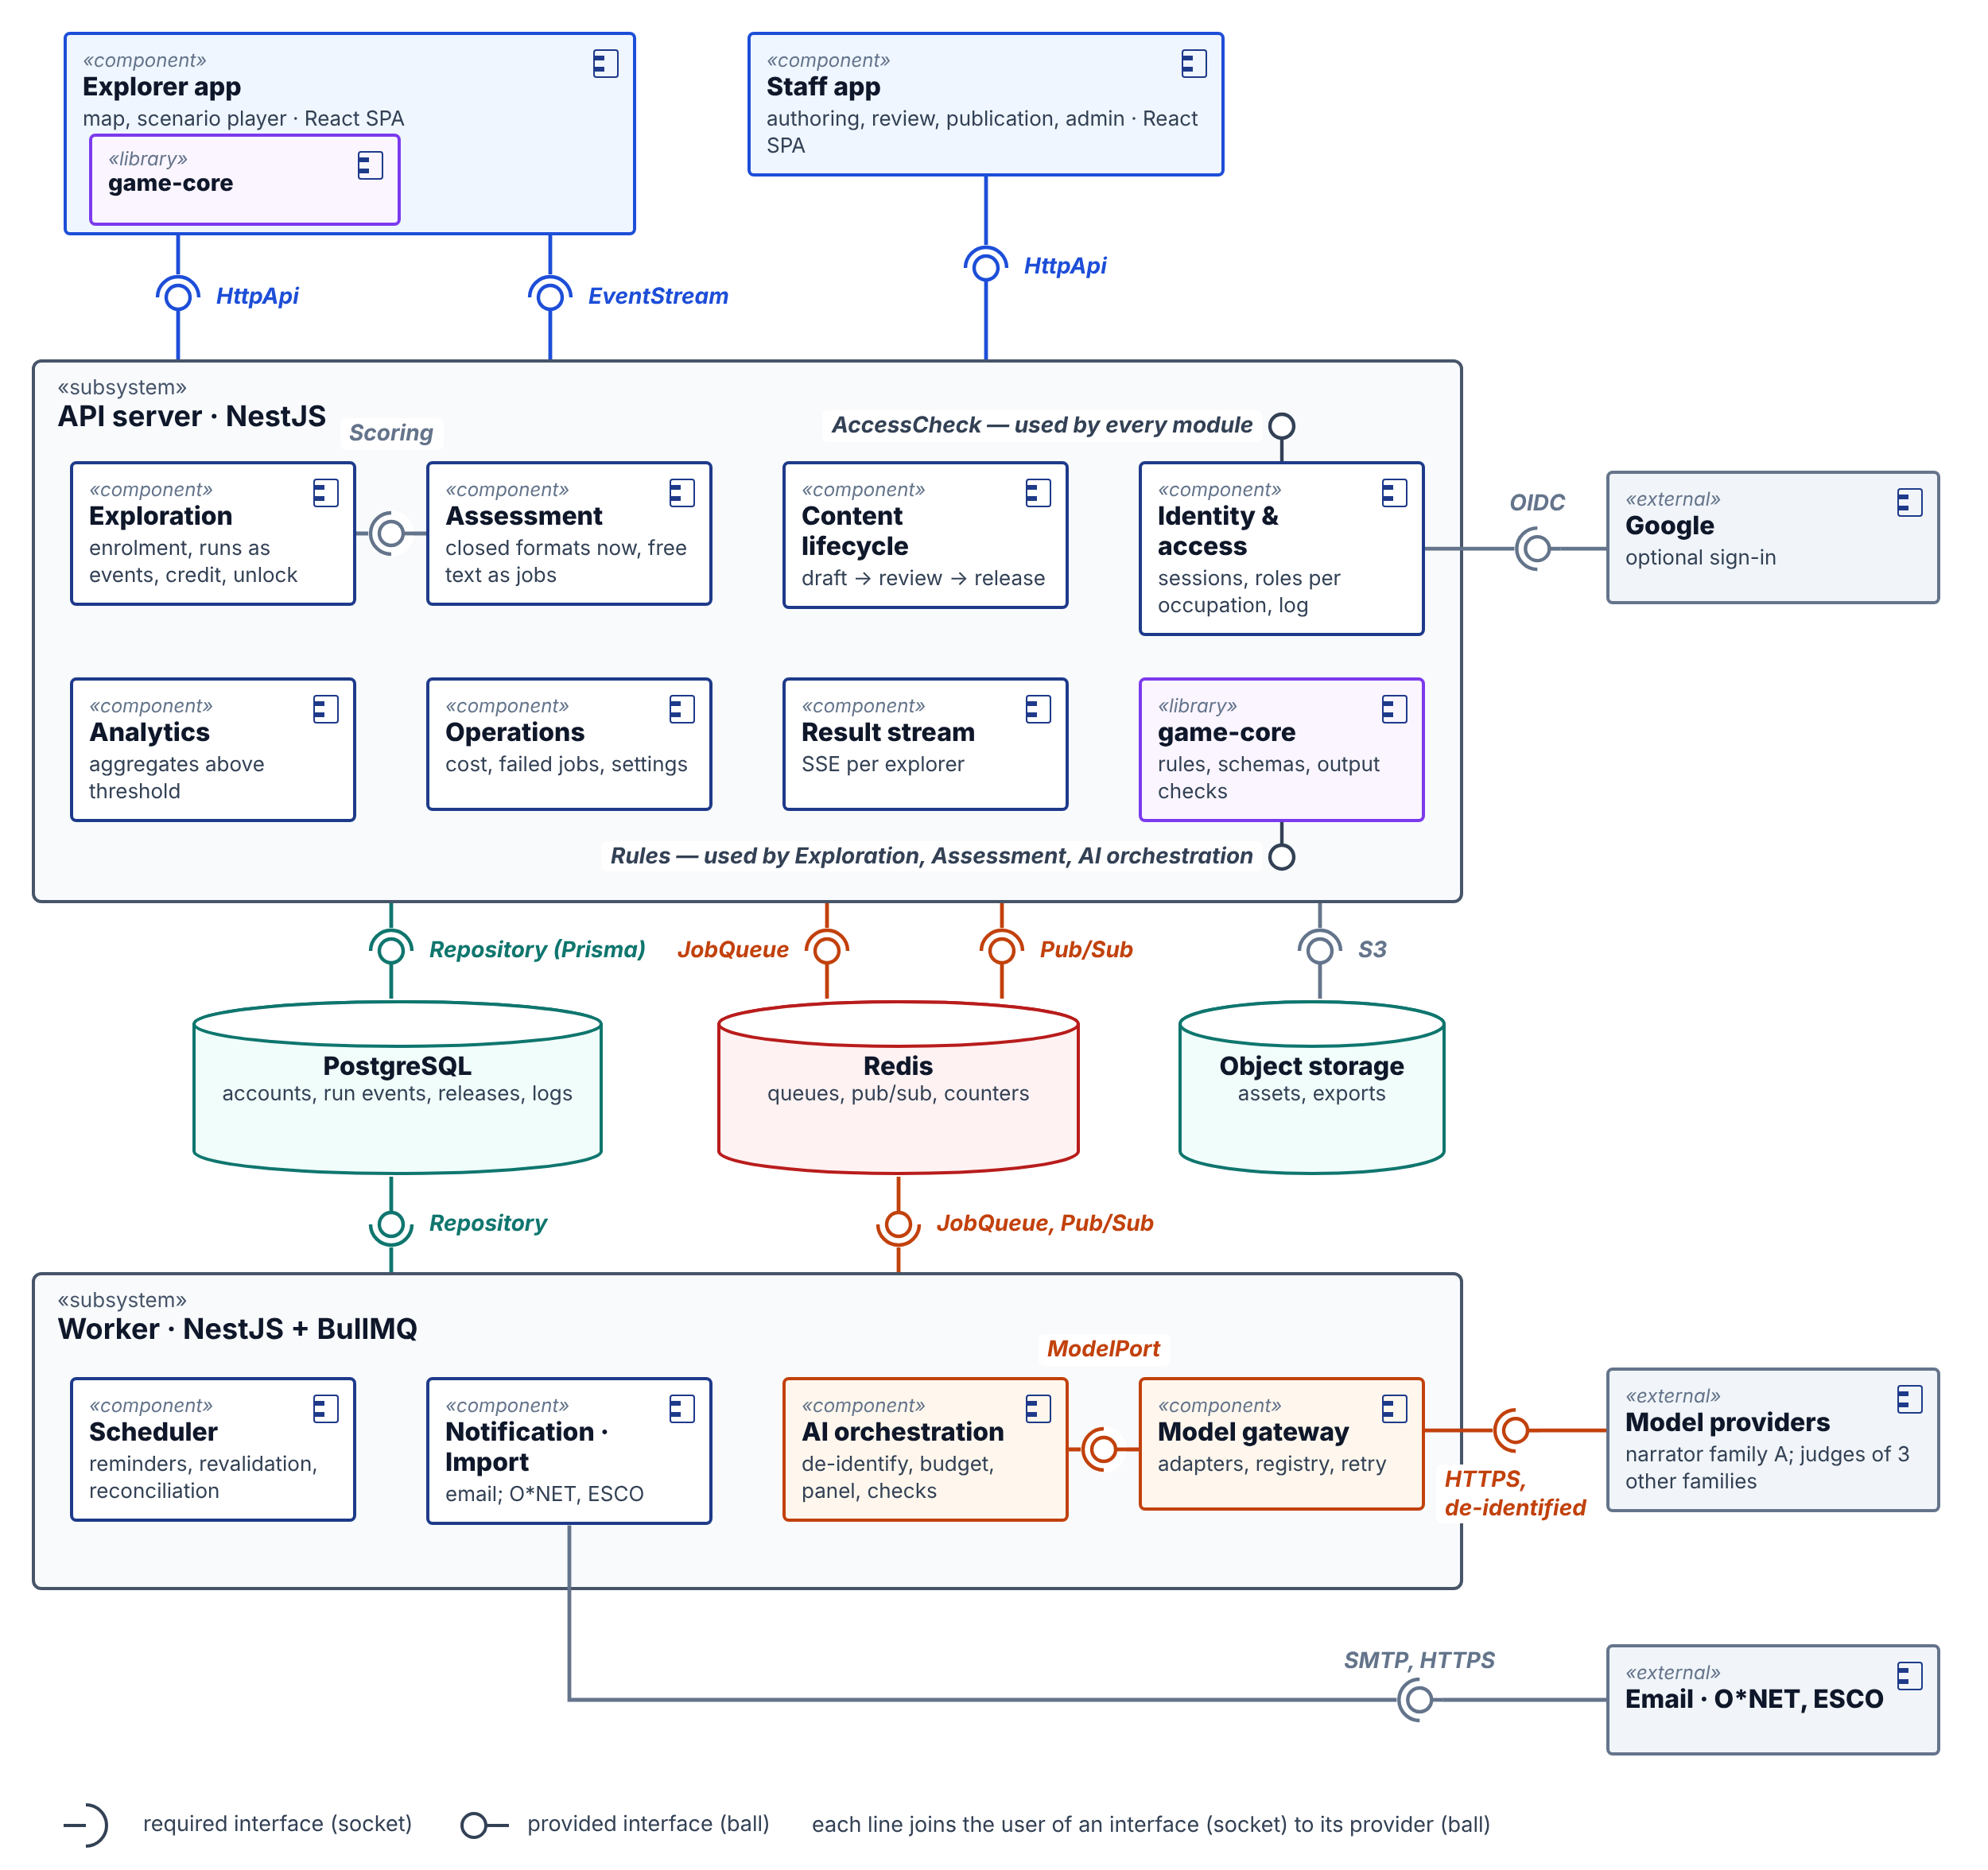
\includegraphics[width=\textwidth,height=0.9\textheight,keepaspectratio]{figures/jobquest_component_diagram.png}
\caption{Component diagram of JobQuest. Each line joins the component that requires an interface (socket) to the component that provides it (ball)}
\end{figure}

Each module is described below with its responsibility and its state in the prototype.

Explorer application. The occupation map, levels, the scenario player for the four response forms of FR-10, hints, follow-ups, results, the personal record, ratings, and feedback (FR-03 to FR-20). It runs \textit{game-core} for instant provisional feedback on closed formats, queues unsent turns locally, and receives narration, follow-ups, and assessment results through a server-sent event stream. Prototype: screens, the 3D map, and the four forms exist; the turn queue, event stream, and 2D map do not.

Staff application. The thirty-three staff use cases: the AI-1 interview through which a domain expert gives the knowledge a seed needs, review, test playthroughs, reliability, and blind rating for domain experts; seed drafting with AI-2, catalogue, presentation, publication, and statistics for content administrators; accounts, model configuration, monitoring, and feedback for system administrators. It shares the sign-in screen and origin with the explorer application (FR-41) but is a separate download. Prototype: absent.

Game core. A library with no framework, network, or storage dependency: the reducer folding run events into state, scoring of closed formats against expert keys, credit with the per-scenario cap, unlocking and adjacency offers, content schemas, and the rule checks on model output of Section 5.2.3 --- numbers and names in narration found in the seed or the player's text, the follow-up count, each judge's quotation found verbatim in the answer, levels within the scale. It runs unchanged in browser and server. Prototype: present; its free-text grader is a synchronous keyword matcher inside the reducer, which must become an asynchronous assessment entering the run as an event.

Identity and access. Accounts, sign-in and recovery, sessions, occupation-scoped roles, disabling, deletion, and the activity log (FR-01, FR-02, FR-40, FR-41); every module asks it whether an actor may act on an occupation. Prototype: registration, email and Google sign-in, rotating sessions, and deletion exist; reset, idle expiry, scoped roles, disabling, and the log do not, and the three prototype roles must become the four actors of Section 4.2.1.

Exploration. Everything outside the assessment itself: orientation, catalogue and profiles, enrolment, runs and their events, credit, unlocking, adjacency offers, side quests, ratings, records, and feedback (FR-03 to FR-09, FR-15 to FR-20). It validates turn events with \textit{game-core} and stores them; each free-text answer is handed to Assessment, which stores it with an assessment request in the same transaction. Prototype: present, but runs are submitted as one batch at the end.

Assessment. Turns answers into results, feedback, and guidance (FR-10 to FR-14). Closed formats are scored synchronously by \textit{game-core}; each free-text answer, follow-up answers included, is graded by the judge panel as soon as it is submitted (AI-5), and only then is a follow-up decided (FR-12). The grade and each activity's checked feedback note are written back as events, and at the end of the scenario the notes are combined into the feedback shown on the summary screen in the three separate parts of FR-14. It also routes explorers' flags of wrong content to the occupation's domain experts. Prototype: closed formats scored by replaying the run; free text matched by keyword.

Content lifecycle. Occupations, knowledge, scenarios and drafts, generation history, review criteria, assignments and decisions, presentation, assets, and publication (FR-21 to FR-38). It is the only writer of content, implements the state machine SM-01, writes each transition with its log entry in one transaction, and publishes immutable, versioned releases. It uses AI orchestration for generation, validation, presentation, and missing assets; the scheduler for deadlines and annual revalidation; and the importer for O*NET and ESCO, whose interest codes also drive orientation matching (FR-03). A domain expert or content administrator can send a published scenario back for revalidation while it stays playable (FR-27). Prototype: versioned immutable documents, written only by a seed script.

AI orchestration. Runs every model use of the five AI components of Section 5.2.3 as a job: the expert interview (AI-1) and seed drafting (AI-2) at authoring time, with presentation design and missing assets (FR-35, FR-36); test playthroughs (AI-3); narration, follow-ups, and feedback notes during play (AI-4, FR-12, FR-14); and grading of each answer by a panel of three judges (AI-5, FR-11). The Get-to-know-me quiz uses no AI (FR-04). Per job it loads the pinned content version, removes identifying details from explorer text, checks the session budget, calls the model port, applies \textit{game-core}'s rule checks, and records model, prompt version, cost, and latency. There is no scripted substitute for a model's output: a job that cannot complete is retried or waits, and a session pauses until it can. It rechecks at job time that no judge shares the narrator's family or another judge's. Prototype: absent; queue and model-client libraries are declared but unused.

Model gateway. One adapter per provider and a registry recording each model's role --- text generation, assessment, image generation (FR-36) --- with its provider and family; configuration is refused when the narrator and a judge, or two judges, share either (FR-42, DC-01). It applies per-provider concurrency limits, timeouts, retries, and a circuit breaker. Adapters are written by the project over the OpenAI-compatible format, with native adapters where that format falls short (Section 5.2.3). Prototype: absent.

Analytics. Everything shown only in aggregate: ratings and statistics above the population threshold, play-tests excluded (FR-19, FR-39, NFR-06, DR-11); coverage; agreement by difficulty stratum and the disagreement list (FR-28, NFR-14); and blind ratings (FR-29). Occupation ratings are re-aggregated in the transaction that stores each rating (FR-19); heavier statistics refresh periodically, later from a replica. It never returns an individual's record. Prototype: personal summaries only.

Operations. Telemetry of usage, cost, latency, and errors (DR-10); failed jobs and re-runs (FR-43); versioned settings, including the cost ceiling (DR-17); and feedback review (FR-20). Prototype: absent.

Notification, scheduler, and import. Notification sends email and in-app notices: reset links, review assignments, reminders, play-test invitations. The scheduler runs recurring jobs: review reminders and overdue notices (FR-34), annual revalidation (BR-15), retention, refreshing statistics, and the reconciliation that re-queues any narration or scoring request left without a result. The importer loads O*NET and ESCO and lists unresolved records (FR-31). Prototype: absent.

Data stores. The operational database is the system of record: relational tables for accounts, assignments, runs, events, evidence, reviews, ratings, and logs, and documents for content. The queue store holds jobs, rate limits, budget counters, and the publish--subscribe channel feeding event streams --- nothing that cannot be rebuilt from the database. The object store holds assets and exports. Prototype: the database, with 19 tables.

System overview. The figure below shows the whole system as deployed: the two browser applications, the content delivery network, the reverse proxy, the API and worker processes with the modules inside them, the three data stores, and the external services. The dashed border is the boundary of DC-03; only de-identified text crosses it, through the model gateway. The numbered arrows follow one written answer from submission to what the explorer sees, the path detailed below.

\begin{figure}[H]
\centering
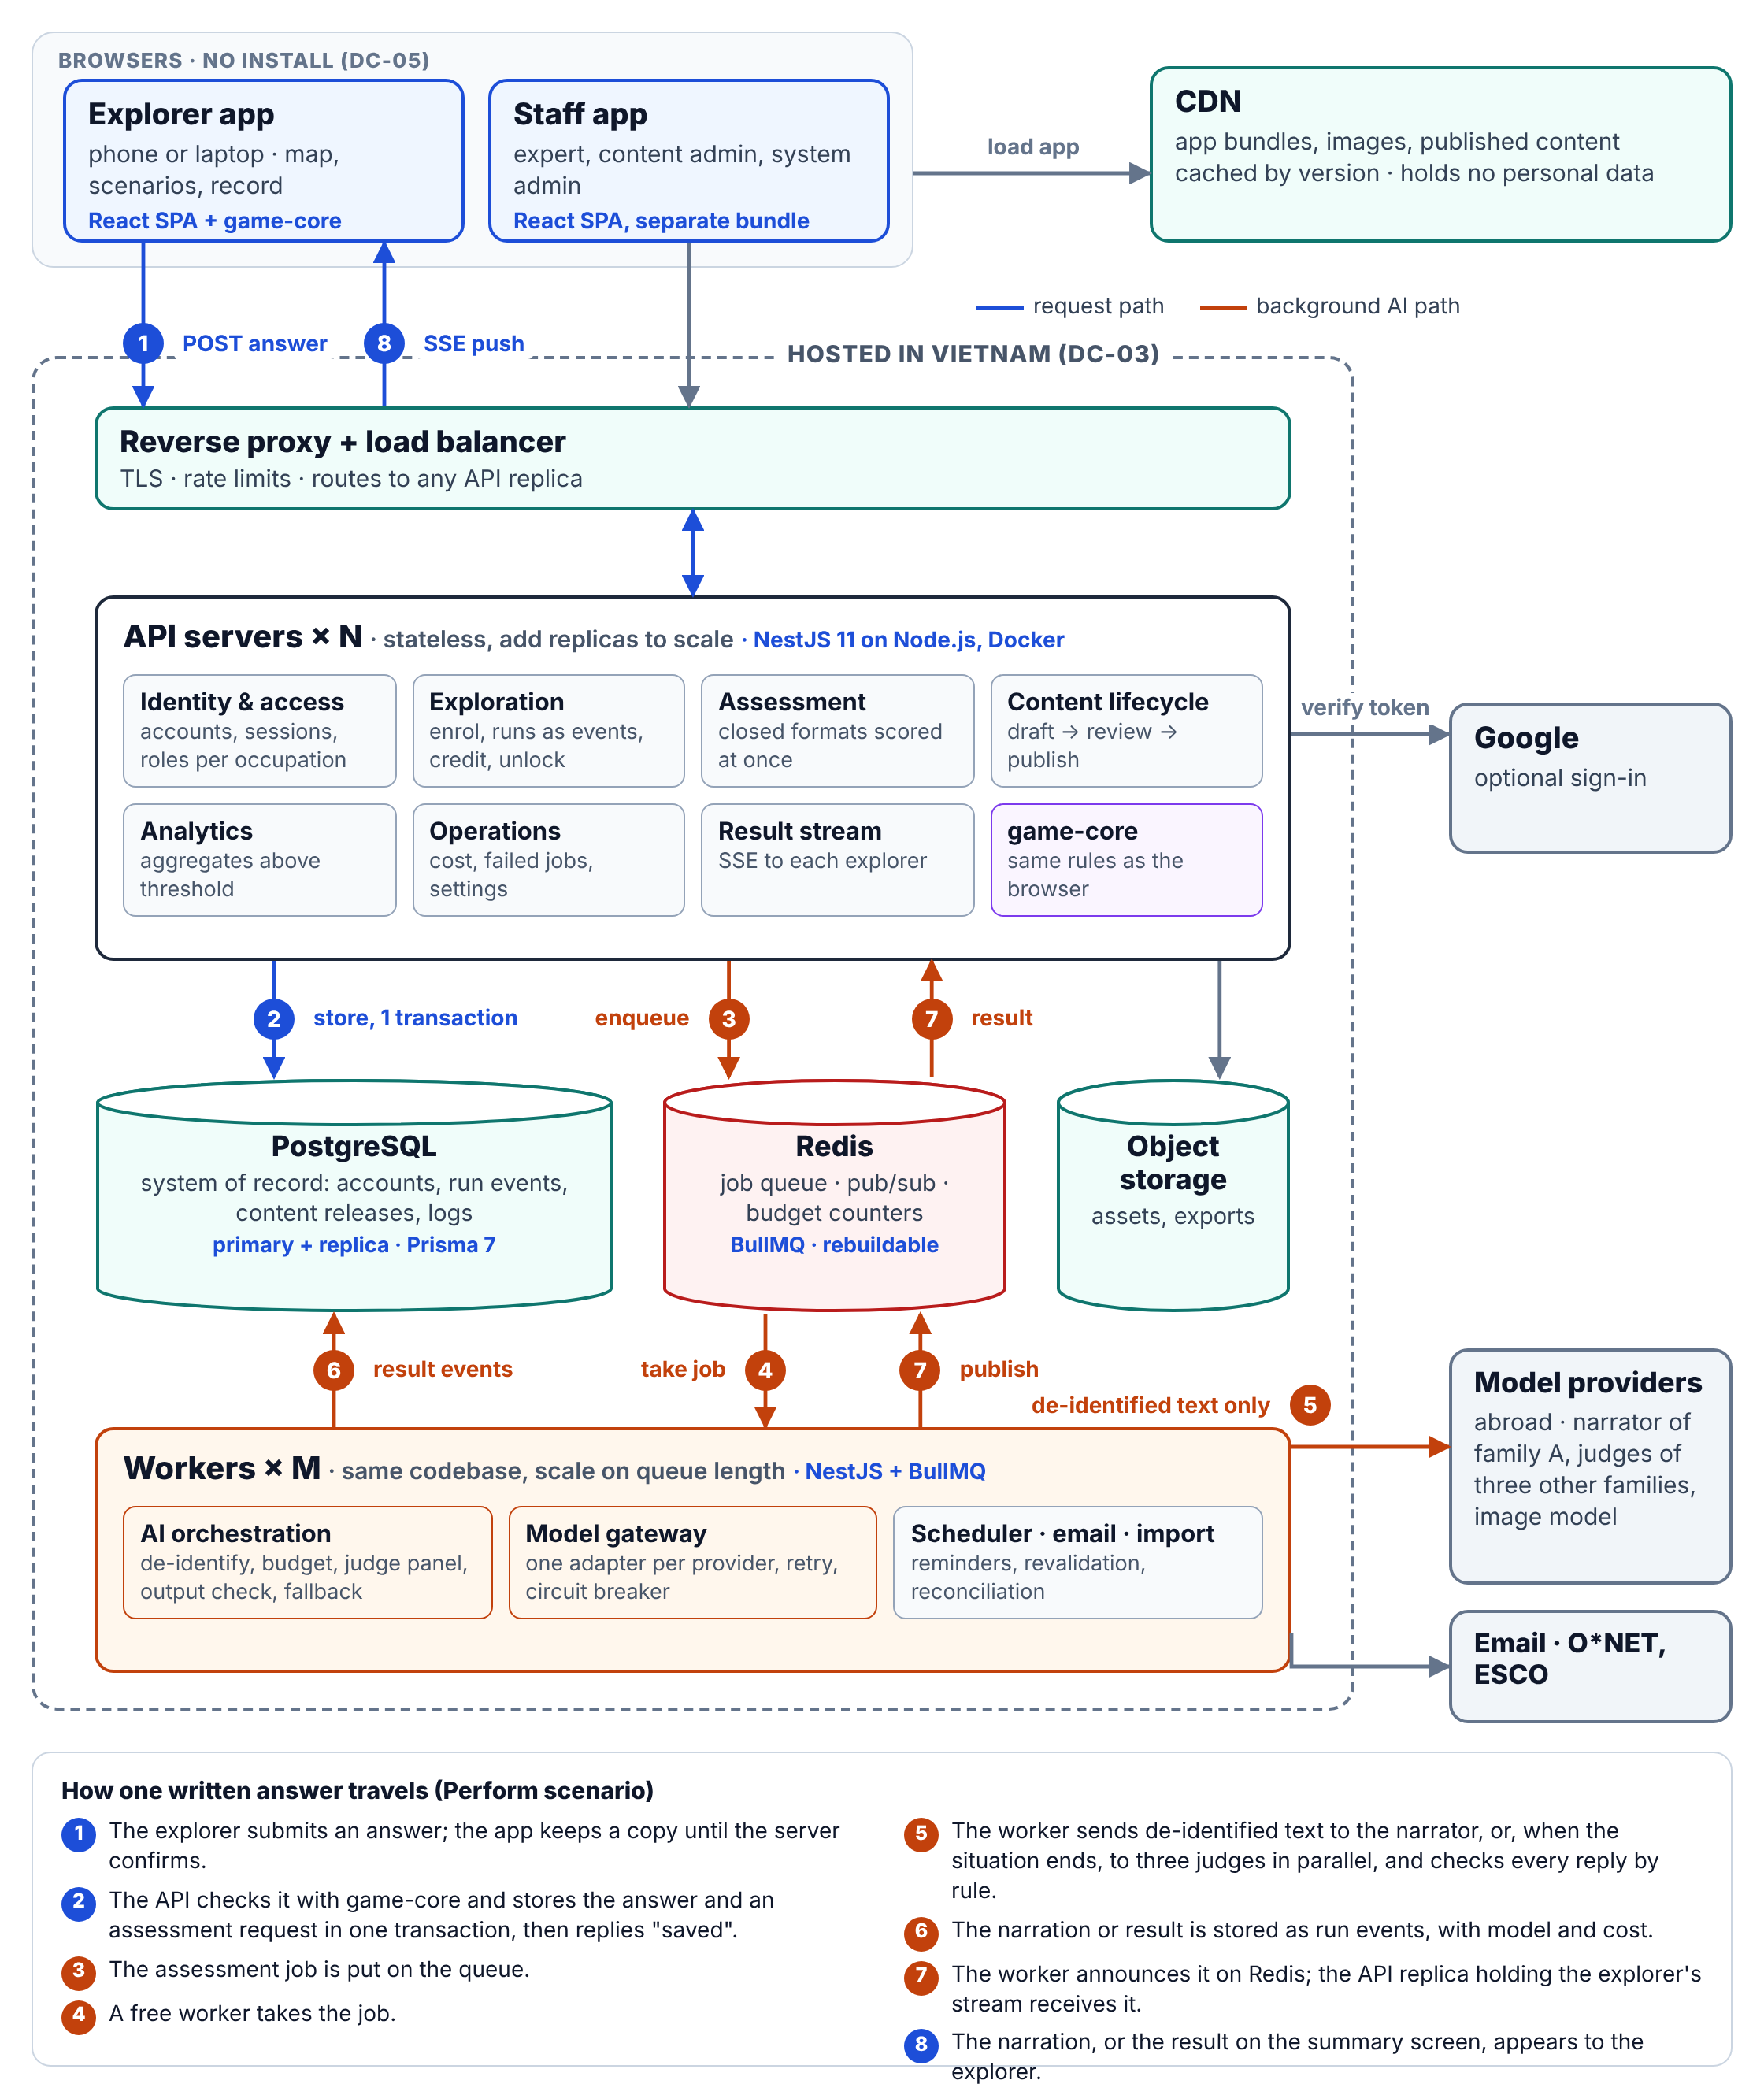
\includegraphics[width=\textwidth,height=0.9\textheight,keepaspectratio]{figures/jobquest_arch_overview.png}
\caption{System overview of JobQuest: components, technologies, and hosting, with the numbered path of one written answer. Blue arrows are the request path; orange arrows the background AI path; the dashed border is the hosting boundary of DC-03}
\end{figure}

Deployment. The deployment diagram below follows UML notation: devices and nodes are drawn as three-dimensional boxes, the artifacts deployed on them as documents inside, and each communication path is labelled with its protocol; the components of Section 5.3.1 appear inside the artifact that manifests them. Both applications are static bundles, served to browsers by a content delivery network that holds no personal data. Inside one cloud region in Vietnam, a web application firewall and load balancer terminate TLS and spread requests over the API pods of two zones. API and worker pods run the same Docker image, started in two roles; both are stateless, so capacity grows by adding pods: API pods on CPU and open streams, worker pods on queue length. PostgreSQL runs as a primary with a synchronous standby in the other zone and a read replica for analytics; Redis runs as a primary with a replica. The model gateway reaches the providers abroad only through an egress proxy that admits allowlisted endpoints, and backups are copied to a second region in Vietnam. An observability node inside the region receives metrics, logs, and traces from the API and worker pods over OpenTelemetry (OTLP), collects metrics from Redis, PostgreSQL, and object storage and logs from the egress proxy, and scrapes the load balancer, so that queue length, latency per provider, and cost per session are watched in one place. At Stage 1 the same nodes run on one university server under Docker Compose, with one API and one worker.

\begin{landscape}
\begin{figure}[H]
\centering
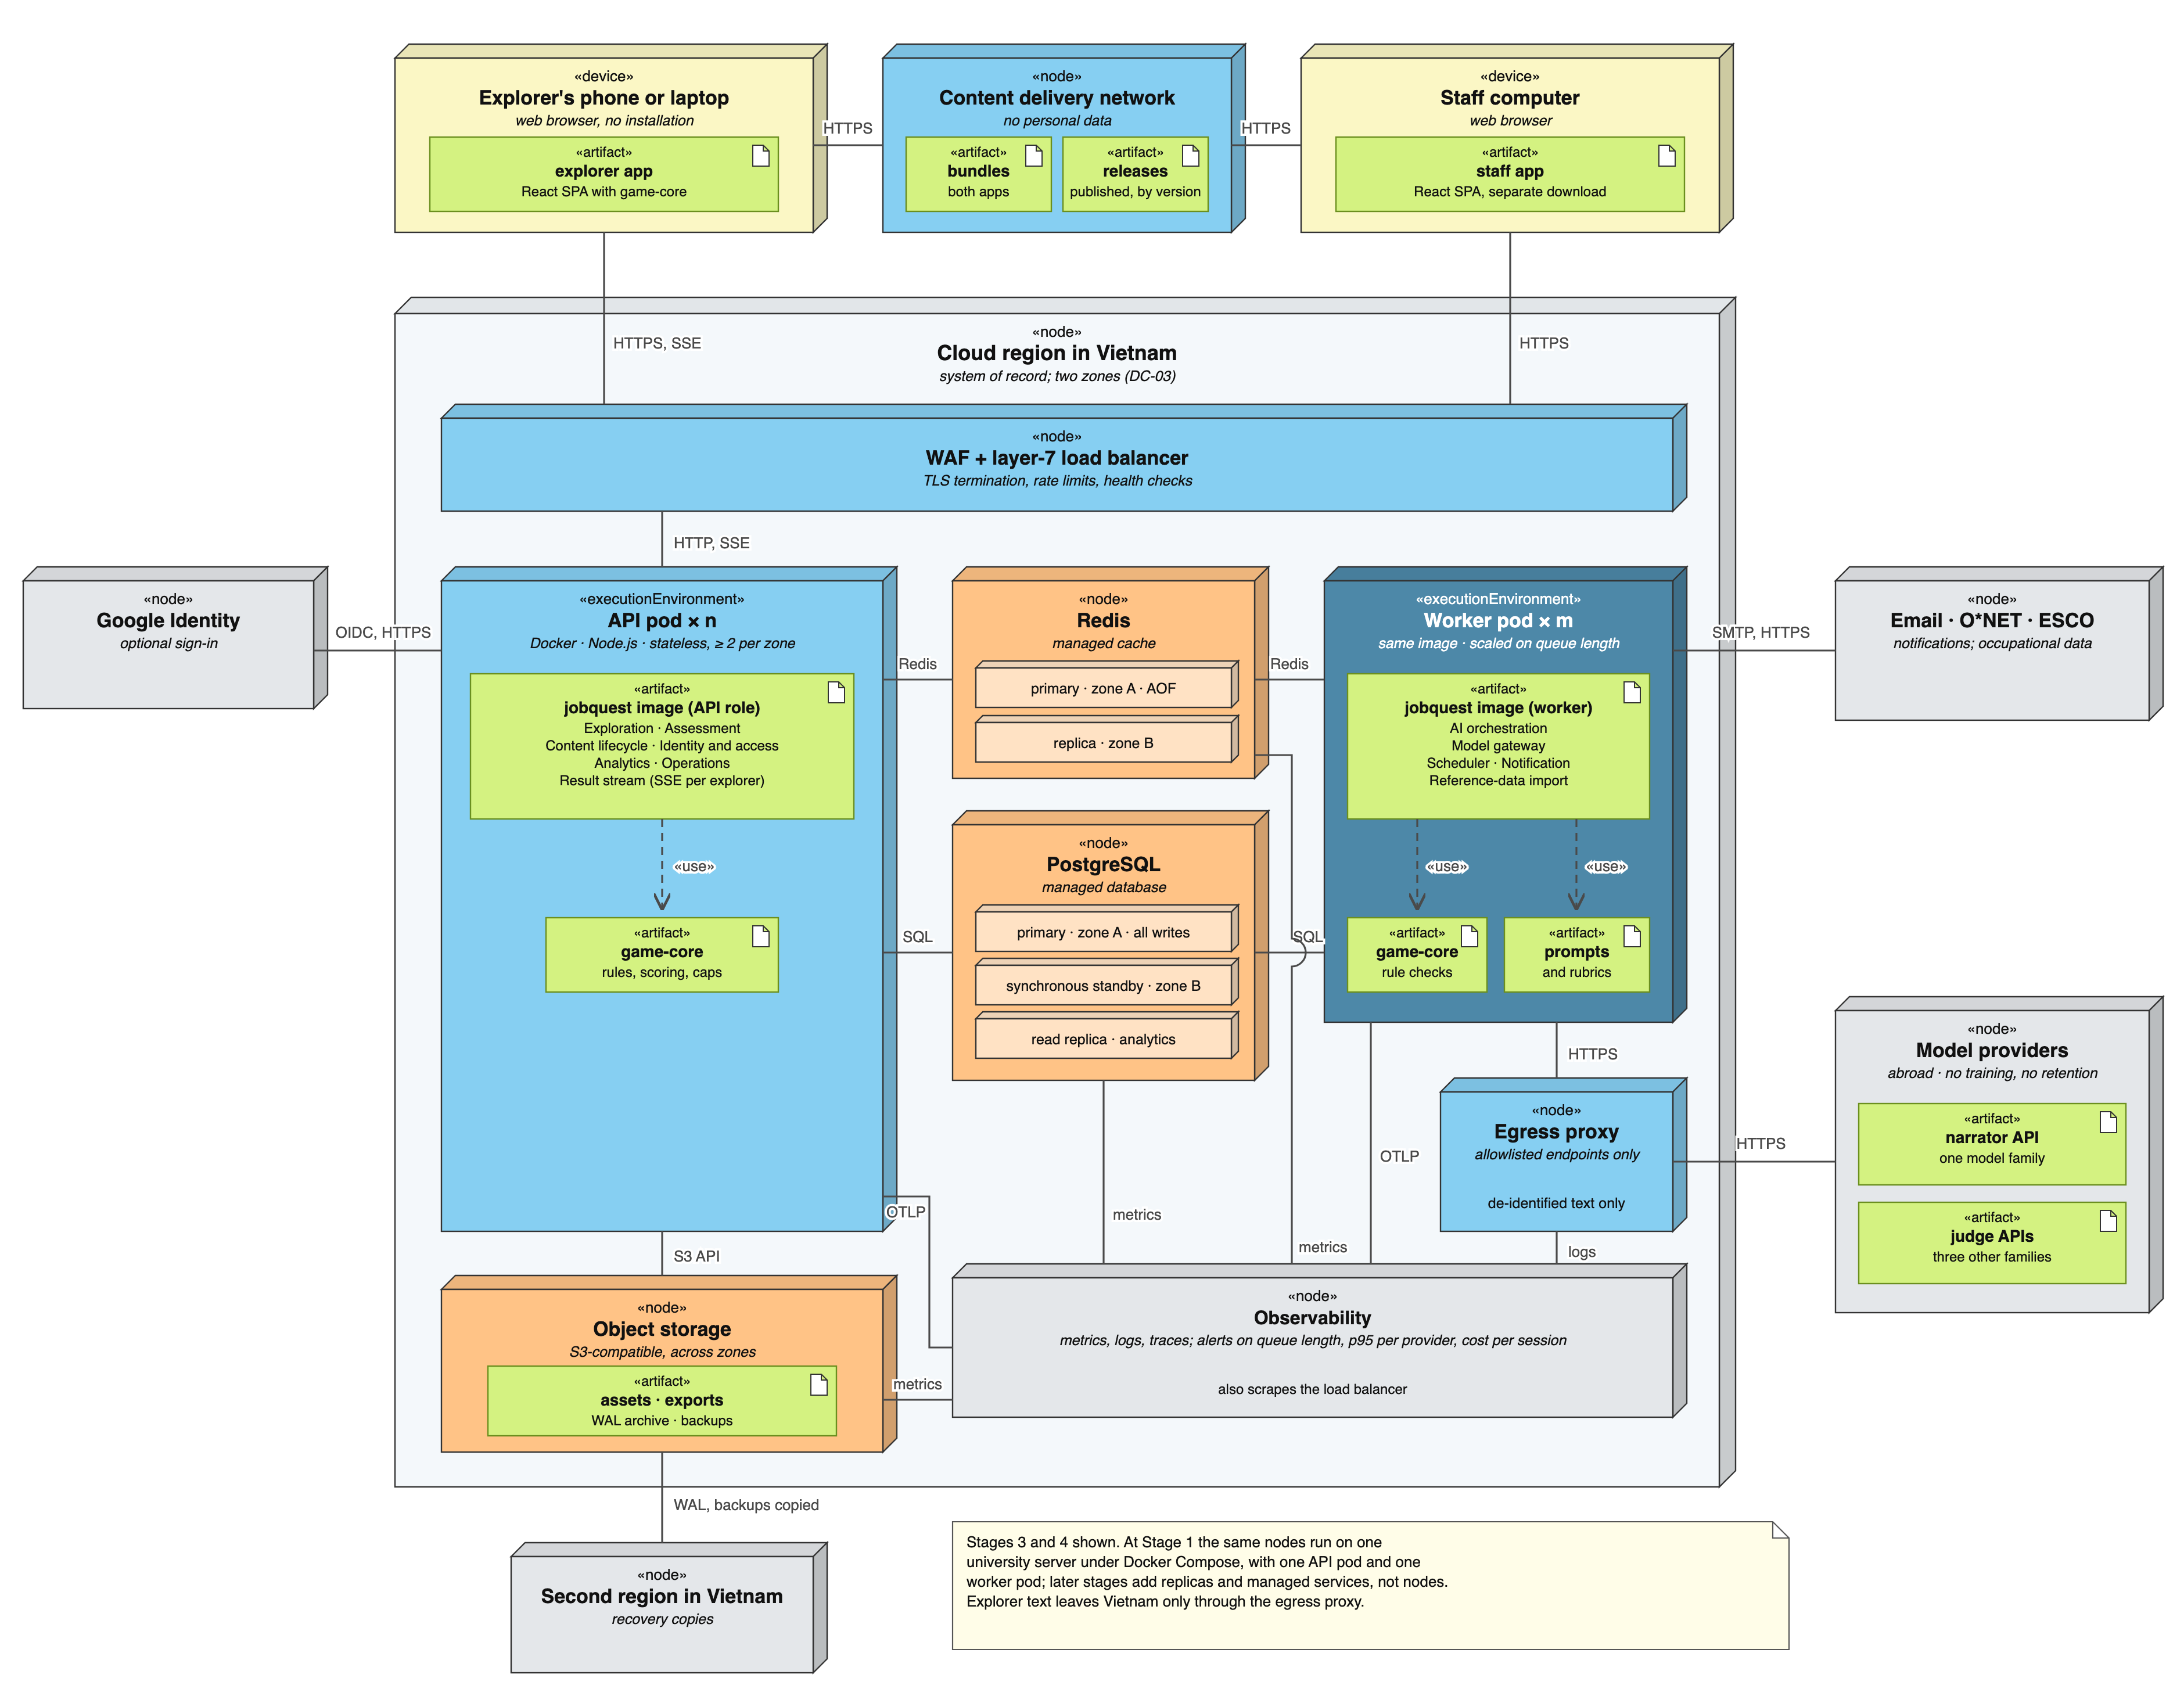
\includegraphics[width=\linewidth,keepaspectratio]{figures/jobquest_deployment.png}
\caption{UML deployment diagram of JobQuest at Stages 3 and 4: devices, nodes, and execution environments, the artifacts deployed on each, and the protocol of each communication path}
\end{figure}
\end{landscape}

The assessed turn. A free-text answer in Perform scenario tests the architecture hardest, because it involves the explorer, the authority over scores, the models, and the failure of any of them. The answer is graded first, by the three judges (AI-5); only then does the narrator decide whether to ask a follow-up (AI-4), and each follow-up answer goes through the same loop. The figure below shows the sequence for one activity.

\begin{figure}[H]
\centering
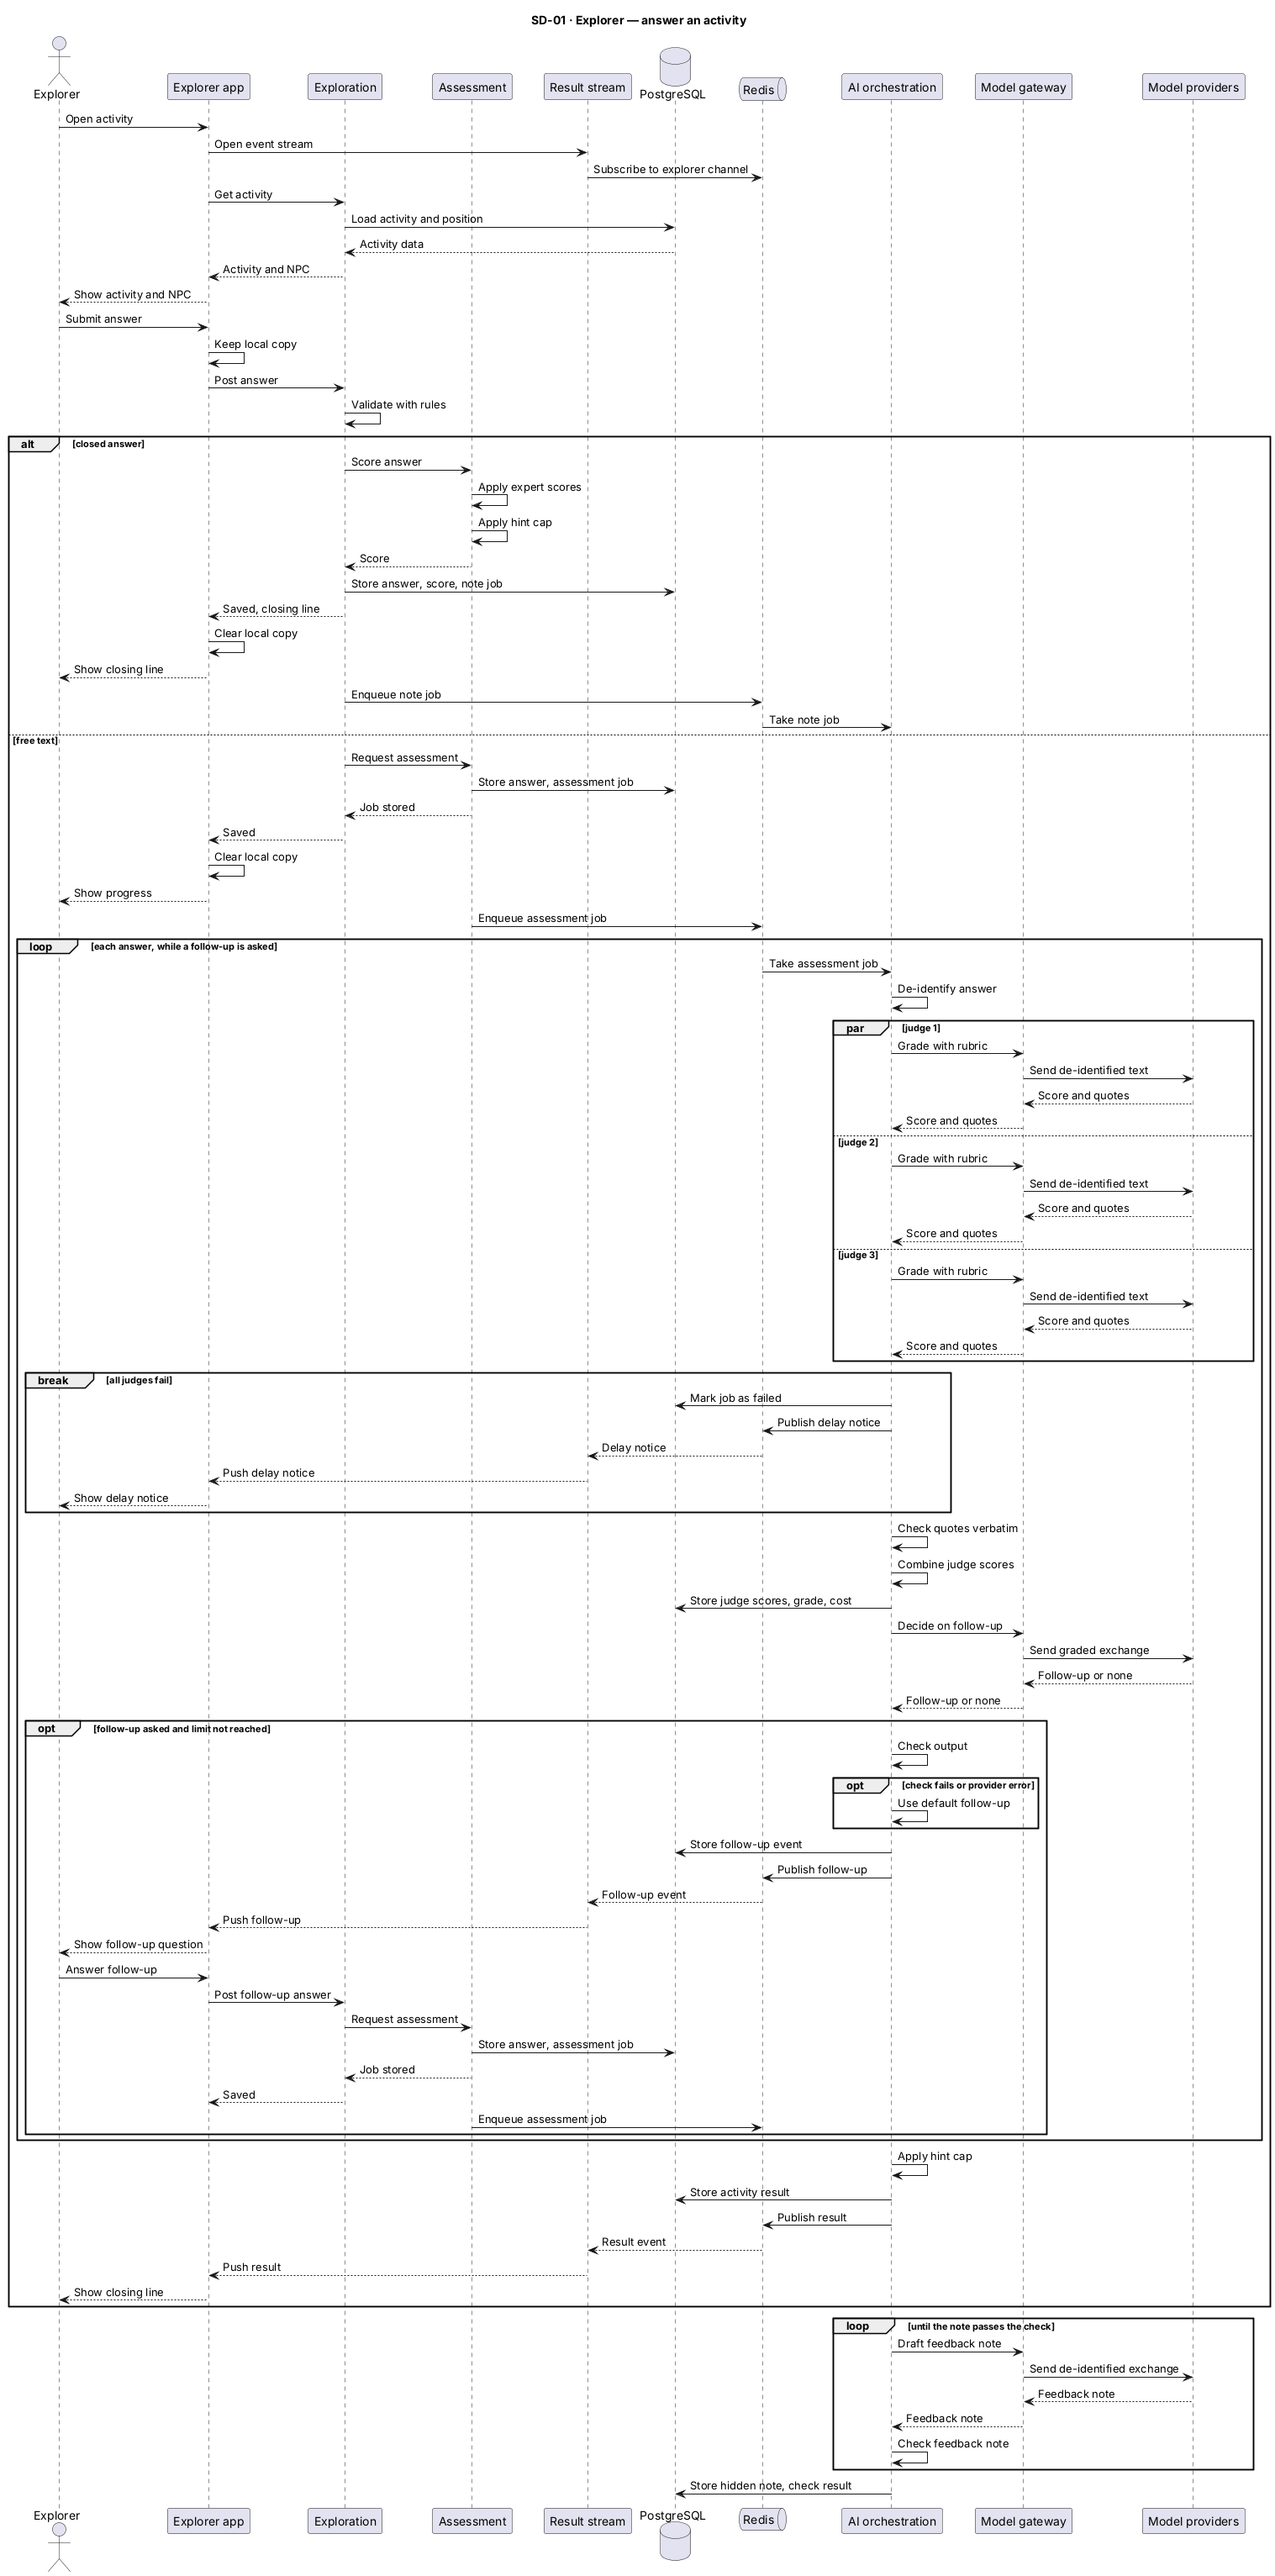
\includegraphics[width=\textwidth,height=0.9\textheight,keepaspectratio]{figures/SD-01_Explorer_AnswerActivity.png}
\caption{Sequence of one activity (SD-01): the answer stored before any model call, grading by three judges in parallel, the follow-up decided after the grade, the activity result pushed to the explorer, and the hidden feedback note drafted and checked}
\end{figure}

\begin{enumerate}[leftmargin=1.5em]
  \item Submission: the explorer application keeps a local copy of the answer and sends it with the run's next sequence number and an idempotency key, so a retry cannot record it twice (NFR-03, NFR-13). Exploration checks it with \textit{game-core}, and Assessment stores it with an assessment request in one transaction and enqueues the job directly after commit --- a transactional outbox\cite{r165} guarantees a job for every stored answer --- before replying that the answer is saved. Progress shows at once, and a status line after two seconds (NFR-01).
  \item Grading: a worker removes identifying details and sends the answer, as delimited data the models are instructed never to obey, to three judges of three families in parallel, at most three criteria per call. Each judge returns, per criterion, a verbatim quotation, a rationale, and a level; a judgment is kept only if the quotation occurs in what the player typed (FR-11, NFR-17). The judges' scores are combined into one grade, judges more than one level apart flag the case for the expert (AI-3), and each judge's score, the grade, and the cost are stored (DR-07).
  \item Follow-up: with the grade known, the narrator is sent the graded exchange and the seed, without the rubric or scoring keys, and returns a follow-up or none. A follow-up is shown only if it passes the rule checks --- numbers and names from the seed or the player's text, follow-ups within the count the engine allows --- and otherwise, or on a provider error, the expert's default follow-up is shown (FR-12, NFR-15). It reaches the explorer through Redis and the event stream, and its answer returns to step 1.
  \item Result: once no further follow-up is asked, \textit{game-core} applies the hint cap and the credit within the cap of BR-11; the activity result is stored as an event with its provenance, and Redis carries it to the API replica holding the explorer's stream, which shows the NPC's closing line. Each event carries its sequence number, so a reconnecting stream replays whatever it missed from the database.
  \item Feedback note: a further job asks the narrator for a hidden feedback note built from the rubric anchors, checks it, and redrafts it until it passes; the note is stored with its check result (FR-14, DR-07). At the end of the scenario the notes are combined, and result, feedback, and guidance appear as separate parts on the summary screen.
  \item Failure: the gateway retries, then switches to another model in the same role: another narrator model for narration, and for a judge the other tier of the same family, so that the panel keeps three families (DC-01); this is still AI (DC-02). If every judge fails, the job is marked as failed and the explorer receives a delay notice within ten seconds (NFR-04); the session pauses with every answer and all progress saved, play resumes when a model is available again, and pages that do not use AI, such as sign-in, the map, and the record, stay available. The scheduler re-queues any request left without a result, so not even loss of Redis loses an answer.
\end{enumerate}

A closed-format answer skips steps 2 and 3: the client shows \textit{game-core}'s score at once, the server recomputes it from the stored event, and the feedback note is still drafted for the activity. Resuming after an interruption (flow 7c) folds the stored events and returns the state at the last recorded position on any device.

Content path. The figure below shows the path a scenario takes from opening to play, and the two ways it returns to review.

\begin{figure}[H]
\centering
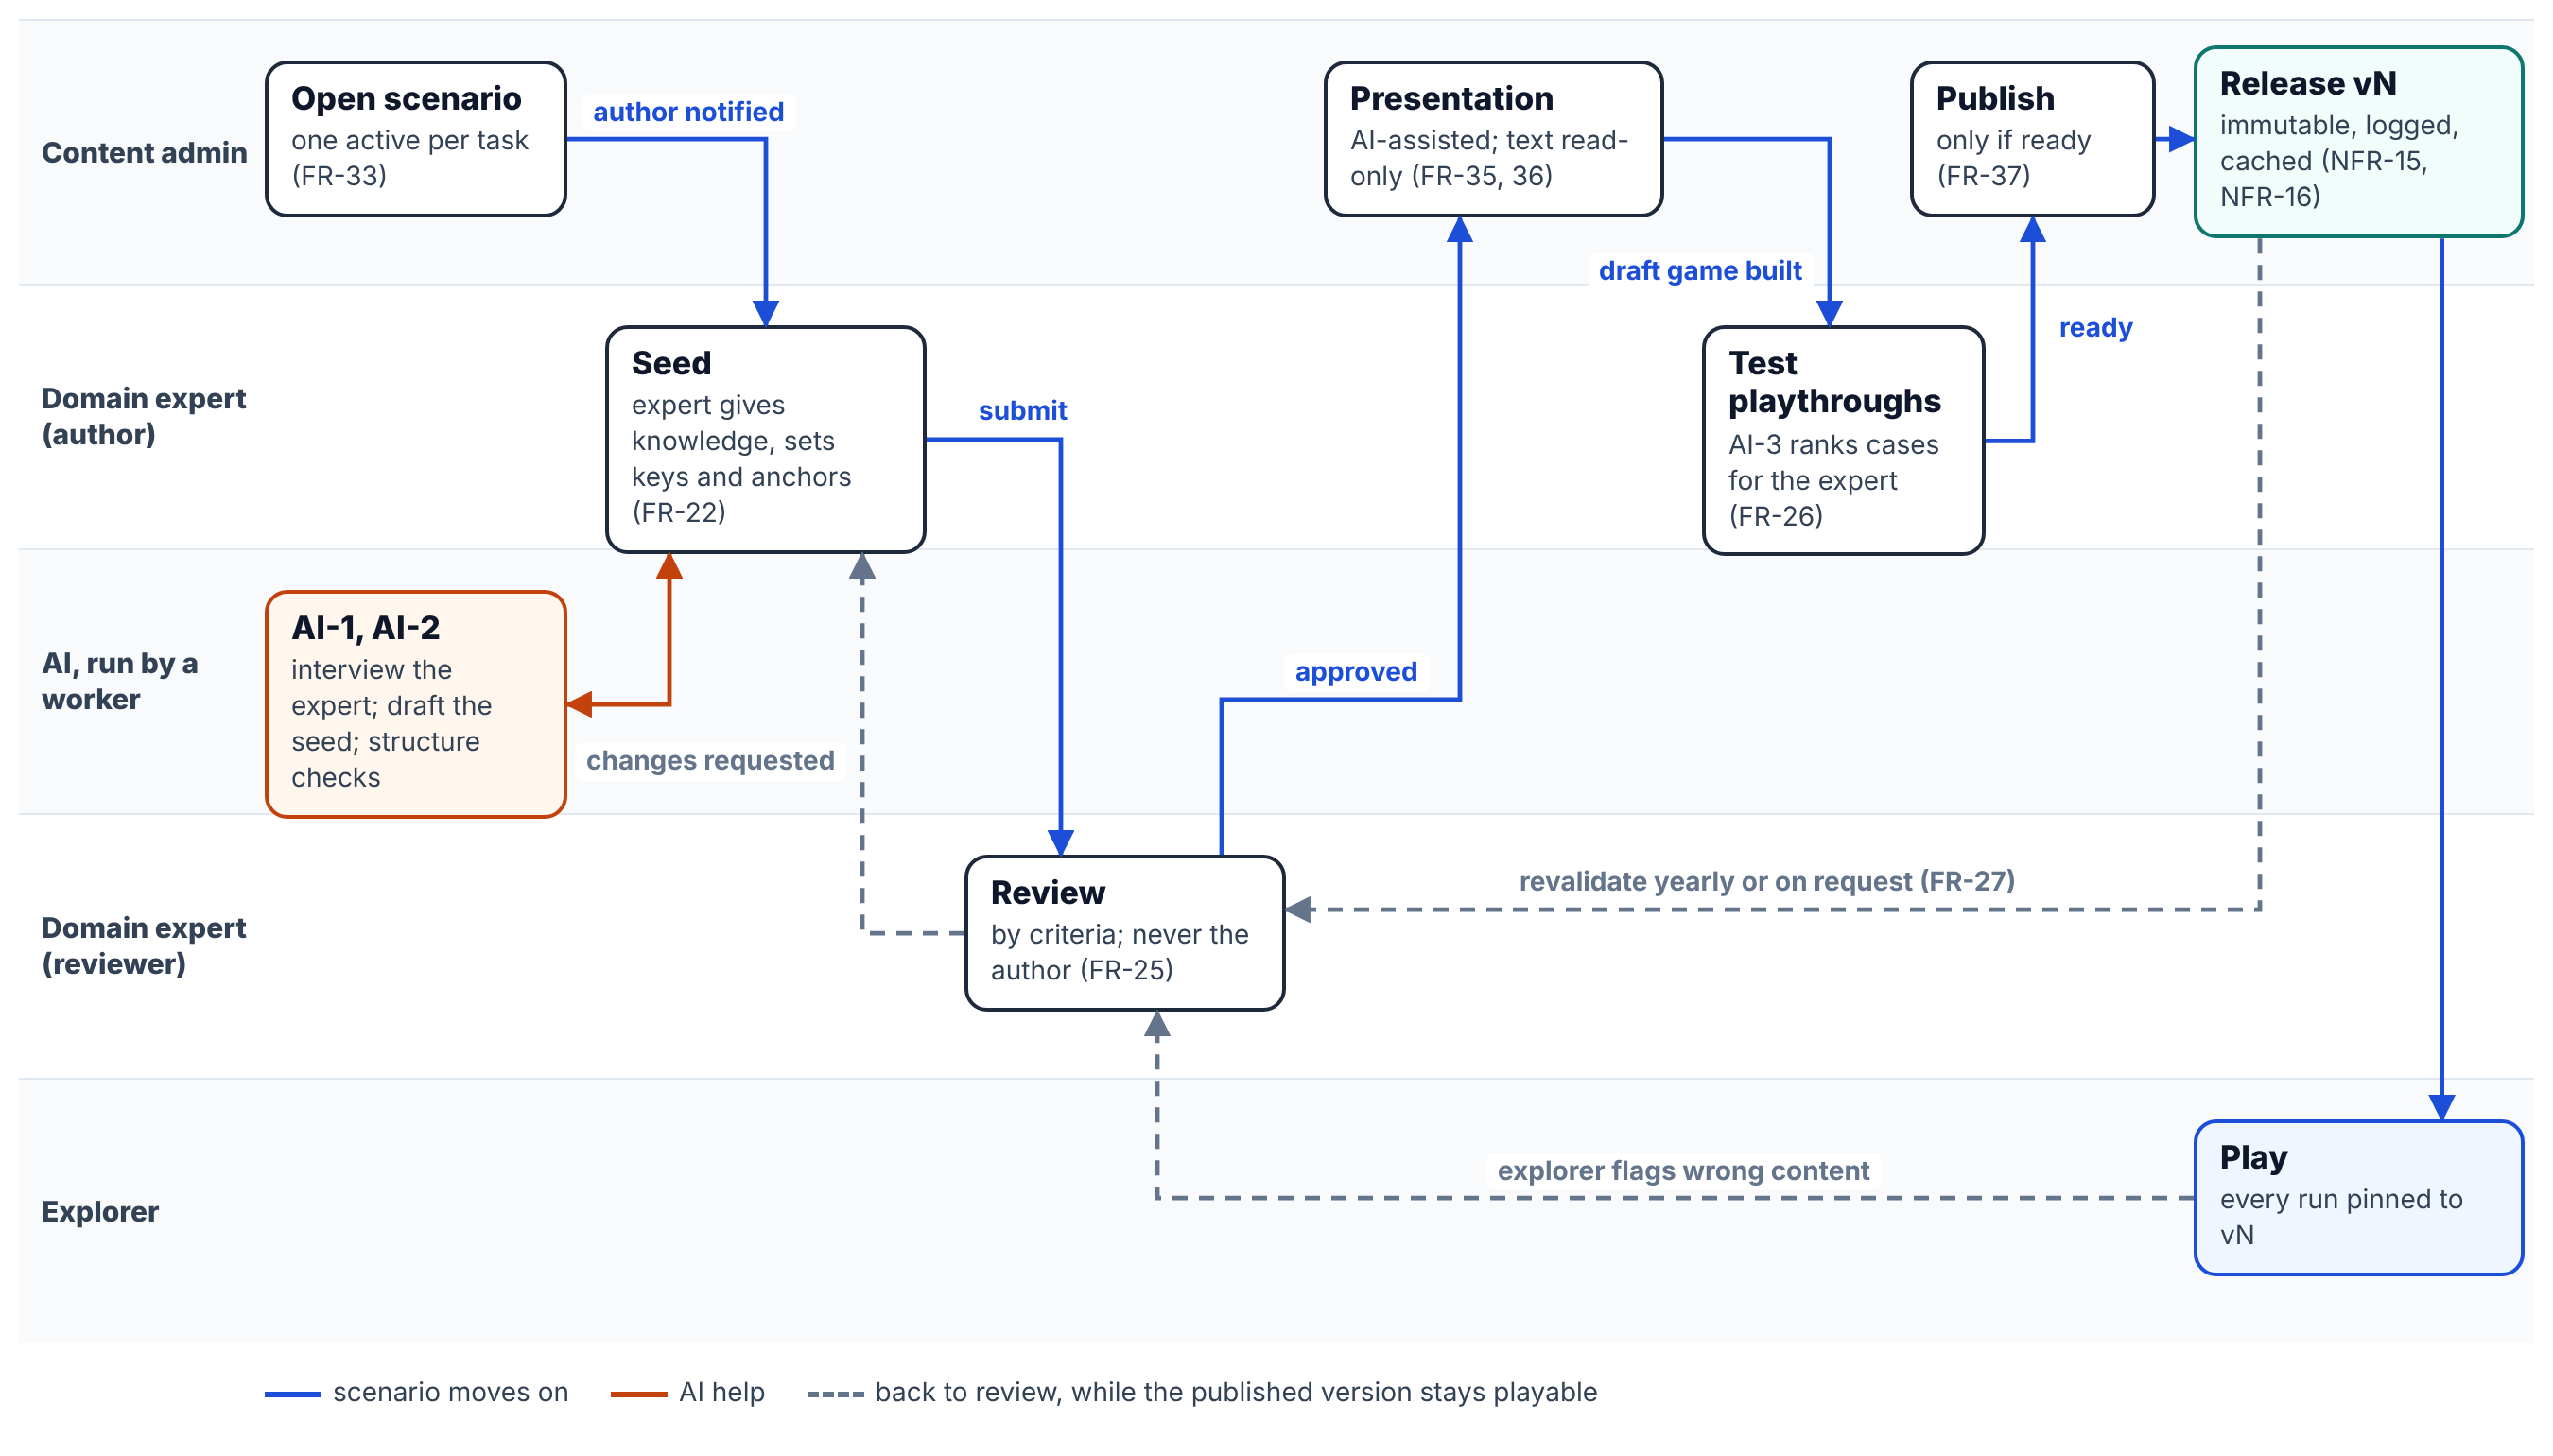
\includegraphics[width=\textwidth,height=0.9\textheight,keepaspectratio]{figures/jobquest_content_lifecycle.png}
\caption{Content lifecycle of a scenario, by actor: the expert's knowledge collected by AI-1 and drafted into a seed with AI-2, review by another expert, presentation, test playthroughs ranked by AI-3, and publication as an immutable release; revalidation and explorers' flags return it to review while the published version stays playable}
\end{figure}

Latency budget. Under the Lighthouse mobile profile\cite{r137}, the platform's own share of each model step is about 0.4 s: a 150 ms round trip to submit, 20 ms for the transaction, 10 ms to enqueue, 50 ms of preparation and checks, 20 ms to store the result, and half a round trip to push it. That leaves about 7.6 s of NFR-02's eight seconds for the judging panel, and about 4.6 s of NFR-01's five seconds for the narrator to write a follow-up, the budgets against which Section 7.3 measures candidate models; because the panel waits for all three judges, its time is that of the slowest. Since a follow-up is decided only after the answer is graded, the explorer's wait for a follow-up after a free-text answer includes both steps; whether NFR-01 counts from the submission or from the grade is to be settled with those measurements. Generated text is not streamed token by token, because it must pass the rule checks before display.

Realisation of the use cases. The table traces each group of use cases in Section 5.1.2 to the components that realise it.

{\small
\begin{longtable}{|>{\raggedright\arraybackslash}p{\dimexpr 0.316\textwidth-2\tabcolsep-\arrayrulewidth\relax}|>{\raggedright\arraybackslash}p{\dimexpr 0.232\textwidth-2\tabcolsep-\arrayrulewidth\relax}|>{\raggedright\arraybackslash}p{\dimexpr 0.447\textwidth-2\tabcolsep-\arrayrulewidth\relax}|}
\caption{Realisation of use cases by architectural components.} \\
\hline
\textbf{Use cases} & \textbf{Components} & \textbf{Mechanism} \\ \hline
\endfirsthead
\hline
\textbf{Use cases} & \textbf{Components} & \textbf{Mechanism} \\ \hline
\endhead
Register account; Manage account & Explorer application; Identity and access; Notification & Own authentication module; single-use reset links by email \\ \hline
Complete Get-to-know-me quiz; Build user portrait & Explorer application; Exploration & RIASEC matching in \textit{game-core} without AI; fixed portrait text for the highest-scoring type loaded from the database and labelled as self-reported (FR-04, DR-12) \\ \hline
Explore occupations; View occupation profile; View level description; View career path; Enter adjacent occupation & Explorer application; Exploration; Analytics; Game core & Map model from the published release; 3D or accessible 2D rendering; adjacency offers computed by \textit{game-core} from DR-02 and DR-03; ratings with suppression \\ \hline
Choose scenario; Complete side quest & Exploration; Game core & Enrolment and credit in the database; thresholds and caps evaluated by \textit{game-core} on the server; adjacency precomputed from imported data \\ \hline
Perform scenario; View scenario context; Get hint; Resolve activity; Answer follow-up question; Flag wrong content & Explorer application; Exploration; Assessment; AI orchestration; Model gateway & The assessed turn above; flags routed to the occupation's domain experts \\ \hline
Rate occupation; View personal record; Send app feedback & Exploration; Analytics; Operations & Ratings only after completion, aggregated on write; records rebuilt from events; feedback stored with app version \\ \hline
Manage occupation profile; Author scenario; Generate scenario content; Build reference set & Staff application; Content lifecycle; AI orchestration & Drafts with authorship; generation jobs with history and automatic validation; reference answers validated on entry \\ \hline
Review scenario; Apply review criteria; Revalidate scenario; Review flagged content; Play-test draft game & Staff application; Content lifecycle; Exploration; Notification; Scheduler & State machine with reviewer-is-not-author constraint; criteria versioned per review; play-test runs excluded from aggregates \\ \hline
Check grading reliability; Submit blind ratings & Staff application; Analytics; Assessment & Agreement by stratum from recorded judgments; blind ratings hidden from other experts and from AI scores \\ \hline
Manage occupation; Import reference data; Define review criteria; Open task scenario; Assign domain expert; Reassign overdue review & Staff application; Content lifecycle; Reference-data import; Identity and access; Scheduler & One active scenario per task enforced by the database; reviewer and deadline set on assignment, author refused; reminders and overdue notices by the scheduler \\ \hline
Design scenario presentation; Generate missing asset; Publish scenario; Remove scenario & Staff application; Content lifecycle; AI orchestration; Object store & Content text read-only during presentation; task types limited to the domain expert's allowed set; assets checked before entering the library; publication creates an immutable release; deletion retires and keeps history \\ \hline
Monitor occupation statistics; View coverage report; Request revalidation & Staff application; Analytics; Content lifecycle & Aggregates above threshold; revalidation sends a published scenario back to review while it stays playable \\ \hline
Manage user accounts; Assign occupation staff; Disable account; Delete account; View activity log & Staff application; Identity and access & Occupation-scoped roles; status checked on refresh and on every staff request; deletion keeps staff-authored records \\ \hline
Configure AI models; Monitor operation cost; Re-run failed job; Review app feedback & Staff application; Operations; Model gateway & Registry rejects a provider or family shared by the narrator and a judge or by two judges; cost ledger and alerts; failed-job re-run \\ \hline
\end{longtable}
}

Realisation of the non-functional requirements and design constraints. The table gives, for each, the mechanism, the components, and whether the prototype has it; it underlies the verifications listed in Section 4.3.3.

{\small
\begin{longtable}{|>{\raggedright\arraybackslash}p{\dimexpr 0.114\textwidth-2\tabcolsep-\arrayrulewidth\relax}|>{\raggedright\arraybackslash}p{\dimexpr 0.528\textwidth-2\tabcolsep-\arrayrulewidth\relax}|>{\raggedright\arraybackslash}p{\dimexpr 0.204\textwidth-2\tabcolsep-\arrayrulewidth\relax}|>{\raggedright\arraybackslash}p{\dimexpr 0.148\textwidth-2\tabcolsep-\arrayrulewidth\relax}|}
\caption{Realisation of non-functional requirements and design constraints by architectural mechanisms.} \\
\hline
\textbf{ID} & \textbf{Mechanism} & \textbf{Components} & \textbf{In prototype} \\ \hline
\endfirsthead
\hline
\textbf{ID} & \textbf{Mechanism} & \textbf{Components} & \textbf{In prototype} \\ \hline
\endhead
NFR-01 & Answer stored before any model call; narration and follow-up generated by a worker and pushed through the event stream; progress at once, status line after two seconds; interactive jobs before batch generation; bounded output length & Explorer application; Exploration; AI orchestration; Model gateway & No; follow-ups are pre-written \\ \hline
NFR-02 & Assessment job queued as soon as each answer is stored; judges in parallel, so latency is the slowest judge's, not the sum; per-call timeouts; workers scaled on queue depth & AI orchestration; Model gateway; workers & No \\ \hline
NFR-03 & Each turn stored as an event with an idempotent sequence number; local queue of unsent turns; resumption by folding stored events & Explorer application; Exploration; Game core & Partly; runs pinned to a content version, but actions sent only at the end \\ \hline
NFR-04 & Transactional outbox; retries with backoff, circuit breaker, failover within the role; notice within ten seconds; reconciliation & Exploration; AI orchestration; Model gateway; Scheduler & No \\ \hline
NFR-05 & Data inventory per data requirement; encryption in transit and at rest, including backups; de-identification before any model call; opaque job identifiers; providers set to no training and no retention; deletion by cascade & Identity and access; AI orchestration; Operations; database & Partly; deletion by cascade \\ \hline
NFR-06 & Aggregates only from Analytics, above a population threshold; play-tests excluded; no endpoint returns another person's record & Analytics & No \\ \hline
NFR-07 & Every model output carries provenance --- model, family, prompt version --- from which the interface renders an AI label & AI orchestration; Explorer application & No \\ \hline
NFR-08 & Typed interface strings with a completeness test; content fields carry a locale, so a language is added as data; Vietnamese only in this phase & Both applications; Content lifecycle & Partly; interface strings typed \\ \hline
NFR-09 & Validator refuses a scenario whose context lacks an explicit objective & Content lifecycle; Game core & No \\ \hline
NFR-10 & Content as data in releases, created through the staff application; \textit{game-core} interprets generic formats; map positions computed from data & Content lifecycle; Game core; Explorer application & Partly; content in the database, written by script \\ \hline
NFR-11 & Per-session cost ledger: estimate before, actual after each call; ceiling from settings; threshold alerts; a session that reaches the ceiling makes no further model calls and pauses as on provider failure & AI orchestration; Operations; queue store & No \\ \hline
NFR-12 & Model port with provider adapters; provider-neutral prompts and output schemas; a provider change re-runs the Stage A benchmark as a regression suite & Model gateway; AI orchestration & No \\ \hline
NFR-13 & Explorer bundle under a performance budget; on-demand 3D chunk and 2D fallback; turn payloads of a few kilobytes; event stream with polling fallback; releases cached by version at the edge; on-device timing & Explorer application; content delivery network & Partly; 3D map loaded on demand \\ \hline
NFR-14 & Every judgment records its judges; a change of any judge model recomputes agreement by stratum against the reference set & Analytics; AI orchestration; Operations & No \\ \hline
NFR-15 & Publication copies the approved version into a hashed release, compared with what is served; canon content served verbatim; run-time narration shown only after the rule checks, with the expert's default follow-up when a follow-up fails them; feedback notes redrafted until they pass; a model of another family reviews the logs & Content lifecycle; AI orchestration; Game core & Partly; releases immutable \\ \hline
NFR-16 & Lifecycle module as sole writer; transition and log in one transaction; a trigger refuses updates to published releases & Content lifecycle; database & No \\ \hline
NFR-17 & Argon2id; HTTPS with strict transport security; httpOnly, SameSite cookies, rotation, idle expiry; answers passed to models as delimited data, outputs schema-validated; prompt-injection tests in the regression suite, against the leading OWASP risk for language-model applications\cite{r166} & Identity and access; AI orchestration; reverse proxy & Partly; hashing, cookies, rotation \\ \hline
NFR-18 & Stateless API replicas with health checks and rolling deployment; backups with point-in-time recovery; uptime monitoring; announced maintenance & All tiers & No \\ \hline
NFR-19 & Document-based interfaces; accessible 2D map; accessible primitives in the staff application; automated and manual audits & Both applications & No \\ \hline
DC-01 & Registry records each model's provider and family; configuration rejects either shared by the narrator and a judge, or by two judges; panel rechecked at job time & Model gateway; Operations; AI orchestration & No \\ \hline
DC-02 & Domain code depends only on the model port; providers are adapters selected per role & Model gateway & No \\ \hline
DC-03 & System of record in Vietnam; one egress path, through de-identification & Hosting; AI orchestration; Identity and access; Operations & No \\ \hline
DC-05 & Browser applications, no installation; static delivery; tolerant of short disconnections & Both applications & Yes \\ \hline
\end{longtable}
}

Infrastructure and scalability. JobQuest's load is not where web systems usually feel it: the binding constraint is the model tier, not the web or database tier. The estimate below states its assumptions so pilots can revise them. A scenario lasts ten to fifteen minutes (Section 4.1.2) and is assumed to hold three situations, each scored by three judges, plus about four narration and follow-up calls: about thirteen model calls per scenario, or one per minute of play. An active explorer sends a request every five to ten seconds. For Stage 4 the reference is the 1.12 million grade-12 candidates of 2025\cite{r167}: if a fifth of a cohort plays half an hour a week over a ten-week guidance season, concentrated in about twenty peak hours, peak concurrency is about five thousand.

{\footnotesize
\begin{longtable}{|>{\raggedright\arraybackslash}p{\dimexpr 0.158\textwidth-2\tabcolsep-\arrayrulewidth\relax}|>{\raggedright\arraybackslash}p{\dimexpr 0.148\textwidth-2\tabcolsep-\arrayrulewidth\relax}|>{\raggedright\arraybackslash}p{\dimexpr 0.148\textwidth-2\tabcolsep-\arrayrulewidth\relax}|>{\raggedright\arraybackslash}p{\dimexpr 0.128\textwidth-2\tabcolsep-\arrayrulewidth\relax}|>{\raggedright\arraybackslash}p{\dimexpr 0.108\textwidth-2\tabcolsep-\arrayrulewidth\relax}|>{\raggedright\arraybackslash}p{\dimexpr 0.305\textwidth-2\tabcolsep-\arrayrulewidth\relax}|}
\caption{Capacity estimate and topology by roadmap stage.} \\
\hline
\textbf{Stage} & \textbf{Assumed users} & \textbf{Peak concurrent explorers} & \textbf{API requests per second} & \textbf{Model calls per second} & \textbf{Topology} \\ \hline
\endfirsthead
\hline
\textbf{Stage} & \textbf{Assumed users} & \textbf{Peak concurrent explorers} & \textbf{API requests per second} & \textbf{Model calls per second} & \textbf{Topology} \\ \hline
\endhead
0. University project & Team and synthetic data & Under 10 & Under 5 & Under 1 & One host; all containers; hosted development database acceptable \\ \hline
1. Capstone and first pilot & 100 to 300 volunteers & About 50 & 5 to 10 & About 1 & University host in Vietnam; one API and one worker container; PostgreSQL with point-in-time recovery; Redis with append-only persistence; object store; uptime monitor; CDN for static files \\ \hline
2. Multi-site pilot & About 10,000 in partner schools & About 500, in class-sized bursts & 50 to 100 & About 8 & Cloud in Vietnam; two or more API replicas behind a load balancer; workers scaled on queue length; managed PostgreSQL with standby and read replica; managed Redis; staging \\ \hline
3 and 4. Public-sector partnership and national resource & Hundreds of thousands per year & About 5,000 & 500 to 1,000 & 80 to 90 & Two zones in Vietnam with autoscaling, PostgreSQL high availability, and a recovery region (deployment diagram) \\ \hline
\end{longtable}
}

Each tier scales by its own mechanism, summarised below for Stage 4.

{\small
\begin{longtable}{|>{\raggedright\arraybackslash}p{\dimexpr 0.159\textwidth-2\tabcolsep-\arrayrulewidth\relax}|>{\raggedright\arraybackslash}p{\dimexpr 0.243\textwidth-2\tabcolsep-\arrayrulewidth\relax}|>{\raggedright\arraybackslash}p{\dimexpr 0.291\textwidth-2\tabcolsep-\arrayrulewidth\relax}|>{\raggedright\arraybackslash}p{\dimexpr 0.302\textwidth-2\tabcolsep-\arrayrulewidth\relax}|}
\caption{Scaling mechanism of each tier at Stage 4.} \\
\hline
\textbf{Tier} & \textbf{Load at Stage 4} & \textbf{How it scales} & \textbf{Why it can} \\ \hline
\endfirsthead
\hline
\textbf{Tier} & \textbf{Load at Stage 4} & \textbf{How it scales} & \textbf{Why it can} \\ \hline
\endhead
Content delivery network & All static files and published releases & Cache by version with long lifetimes & Releases are immutable, so caches never need purging and content reads never reach the database \\ \hline
API & 500 to 1,000 requests per second; about 5,000 open result streams & Replicas behind the load balancer, scaled on CPU and open connections; at least two per zone & Stateless: sessions travel in cookies and results arrive through Redis publish--subscribe, so any replica can serve any explorer \\ \hline
Workers & 80 to 90 model calls per second; 250 to 700 in flight & Scaled on queue length; each worker runs many I/O-bound jobs concurrently; in-flight calls capped per provider & Jobs are independent and idempotent; the queue absorbs bursts\cite{r168} \\ \hline
Model providers & About 5,100 requests per minute; 7 to 8 million tokens per minute at about 1,500 tokens per call & Several providers per role within DC-01, so quotas add up; priorities: live grading and narration first, feedback notes next, authoring work last & The binding constraint is isolated in its own tier and limited without slowing the rest \\ \hline
PostgreSQL & Under 500 writes per second; about 0.3 TB of run data per season at about 60 KB per run & Vertical growth behind a connection pooler; read replica for analytics; run events partitioned by month & All transactions stay within one primary; heavy reads move to the replica; old partitions are compressed or archived \\ \hline
Redis & About 100 jobs per second, plus publish--subscribe messages & One primary and one replica & Holds nothing that cannot be rebuilt from PostgreSQL \\ \hline
\end{longtable}
}

The in-flight figure follows from Little's law: 85 calls per second, each lasting three to eight seconds. Two sizing assumptions remain to be measured by the load tests of Chapter 7: if one single-vCPU API replica serves about 300 light requests per second, Stage 4 needs four replicas, six with headroom across two zones; if one worker holds 50 calls in flight, it needs six to fourteen workers.

The architecture scales for seven reasons. Processing tiers are stateless, so capacity grows by adding replicas. Fast and slow work are separated: a request stores and acknowledges in about 0.2 s, and slow work waits in a queue, so a class of forty starting together lengthens the queue rather than overloading the API. The binding constraint, the model tier, is isolated and limited on its own. Published content is immutable and therefore almost entirely served from cache. Reads for statistics are separated from writes by a replica. Load is shed by priority rather than by failure: under pressure, live grading and narration go first, feedback notes wait a little longer for the summary screen, and authoring work waits for quiet hours. And no transaction spans services, so growth never requires distributed coordination. Canon content is approved once and served verbatim from releases, so run-time model calls are limited to narration, follow-ups, feedback notes, and grading; the cost per playthrough is estimated in Section 5.2.3.

Reliability and operations. Availability of 99.5\% a month is proposed for Stages 1 and 2 and 99.9\% once two zones run (NFR-18). The write-ahead log is archived continuously and backups taken nightly, both copied to a second region in Vietnam, for a proposed recovery point of five minutes and recovery time of one hour. Deployments roll replica by replica behind health checks, with backward-compatible migrations so old and new versions run side by side. Monitoring tracks queue length, 95th-percentile latency per provider, cost per session, and error rates, alerting at the thresholds of NFR-01, NFR-02, and NFR-11. A web application firewall and TLS guard the entry, secrets are held in a secret manager, and the egress proxy admits only allowlisted model endpoints.

From the prototype to the target. Four prototype mechanisms are kept: rules in a framework-free \textit{game-core} shared by client and server; the server as score authority; content in versioned, immutable releases pinned to each run; and httpOnly cookie sessions with rotating refresh tokens. Six changes reach the target: free-text assessment becomes an asynchronous job whose result enters the run as an event; runs are submitted turn by turn (NFR-03); content is written through the lifecycle module instead of a seed script; three roles become four occupation-scoped actors; the staff application, AI orchestration, gateway, queue, workers, and scheduler are added; and the accessible 2D map is added. Each change extends a prototype component along a boundary it already has; none discards one.

\setcounter{subsubsection}{9}

\subsubsection{Policies for the Processing of the Proposed System and Third Parties}

This section sets the rules under which JobQuest processes personal data and shares any data with third parties, completing the policies of Section 4.1.4. Its central problem is a conflict between two parts of the design. The system of record must be in Vietnam (DC-03), as Vietnam's Law on Personal Data Protection and its implementing decree require\cite{r99,r100}; but scoring and narration depend on language models whose providers all process requests outside Vietnam. Under the law, using a platform abroad to process data collected in Vietnam is a transfer of personal data abroad, whichever region the provider is asked to use. The policies below decide what may cross that border, under what conditions, and what the platform owes its users when it does.

Third parties and what they receive. The table lists every third party the platform deals with, what it receives, and where.

{\small
\begin{longtable}{|>{\raggedright\arraybackslash}p{\dimexpr 0.171\textwidth-2\tabcolsep-\arrayrulewidth\relax}|>{\raggedright\arraybackslash}p{\dimexpr 0.226\textwidth-2\tabcolsep-\arrayrulewidth\relax}|>{\raggedright\arraybackslash}p{\dimexpr 0.290\textwidth-2\tabcolsep-\arrayrulewidth\relax}|>{\raggedright\arraybackslash}p{\dimexpr 0.159\textwidth-2\tabcolsep-\arrayrulewidth\relax}|>{\raggedright\arraybackslash}p{\dimexpr 0.148\textwidth-2\tabcolsep-\arrayrulewidth\relax}|}
\caption{Third parties and the data they receive.} \\
\hline
\textbf{Third party} & \textbf{Purpose} & \textbf{What it receives} & \textbf{Where} & \textbf{Personal data} \\ \hline
\endfirsthead
\hline
\textbf{Third party} & \textbf{Purpose} & \textbf{What it receives} & \textbf{Where} & \textbf{Personal data} \\ \hline
\endhead
Content delivery network & Serve both applications and published releases & Static bundles and releases & Edge locations, including abroad & None \\ \hline
Google Identity & Optional sign-in & An identity token, only when the user chooses Google & Abroad & Yes, by the user's choice \\ \hline
E-mail provider & Password resets and notices & Address and message & To be chosen with a host in Vietnam & Yes \\ \hline
Model providers & Narration, scoring, feedback, authoring help & Seed content and de-identified answer text, under an opaque run identifier & Abroad & Not by design; residual risk below \\ \hline
O*NET, ESCO & Reference data, imported & Nothing; data flows in only & --- & None \\ \hline
Second region of the cloud provider & Backups and recovery & Encrypted copies of the database and logs & Vietnam & Yes, encrypted \\ \hline
\end{longtable}
}

Options for using foreign models. Four ways to reconcile scoring by language models with data kept in Vietnam were compared.

{\small
\begin{longtable}{|>{\raggedright\arraybackslash}p{\dimexpr 0.171\textwidth-2\tabcolsep-\arrayrulewidth\relax}|>{\raggedright\arraybackslash}p{\dimexpr 0.293\textwidth-2\tabcolsep-\arrayrulewidth\relax}|>{\raggedright\arraybackslash}p{\dimexpr 0.189\textwidth-2\tabcolsep-\arrayrulewidth\relax}|>{\raggedright\arraybackslash}p{\dimexpr 0.191\textwidth-2\tabcolsep-\arrayrulewidth\relax}|>{\raggedright\arraybackslash}p{\dimexpr 0.152\textwidth-2\tabcolsep-\arrayrulewidth\relax}|}
\caption{Comparison of ways to use language models on explorer text.} \\
\hline
\textbf{Criterion} & \textbf{De-identify, then send to providers abroad, treated as a transfer (selected)} & \textbf{Send answers abroad as they are, under consent} & \textbf{Open-weight models served in Vietnam} & \textbf{No language model on explorer text} \\ \hline
\endfirsthead
\hline
\textbf{Criterion} & \textbf{De-identify, then send to providers abroad, treated as a transfer (selected)} & \textbf{Send answers abroad as they are, under consent} & \textbf{Open-weight models served in Vietnam} & \textbf{No language model on explorer text} \\ \hline
\endhead
DC-03, NFR-05 Personal data in Vietnam & $\ominus$ identifiers removed before sending; residual risk in free text & $\circ$ every answer leaves with its author's identity & $\bullet$ nothing leaves & $\bullet$ nothing leaves \\ \hline
RP-2, NFR-14 Scoring quality & $\bullet$ the strongest Vietnamese-capable models (Section 5.2.3) & $\bullet$ & $\ominus$ smaller models; quality to be shown & $\circ$ keyword scoring fails (Section 7.3.3) \\ \hline
TC8, TC9 Cost and feasibility now & $\bullet$ pay per call; no hardware & $\bullet$ & $\circ$ GPU hosting beyond the project's means & $\bullet$ \\ \hline
Legal obligations & $\ominus$ transfer impact assessment and notice & $\circ$ the same, for identified personal data, at scale & $\bullet$ none for transfer & $\bullet$ none for transfer \\ \hline
\end{longtable}
}

\textbf{Decision: de-identify before any model call, send only what the task needs, and treat what is sent as a transfer of personal data regardless.} Removing identifiers is what makes the transfer small; treating it as a transfer anyway is what makes the design safe if de-identification of free text misses something. The law treats data that no longer identifies a person as outside its scope, but a free-text answer can name a colleague, a company, or a place, and the platform cannot prove that every such detail is caught, so it does not rely on that exemption. Models served in Vietnam would remove the transfer altogether; they are recorded as later work, starting from the local fallback of Section 5.3.6, once their scoring quality can be measured against the same thresholds.

What may leave the country. The egress proxy admits a request only to an allowlisted model endpoint, and the request may contain only three things: the seed and rubric of the scenario, which are expert content and contain no personal data; the explorer's answer text after de-identification; and an opaque run identifier that maps to the explorer only inside the platform. Names, usernames, e-mail addresses, dates of birth, account identifiers, and profiles never leave. De-identification removes the explorer's own name, username, and e-mail address, which the platform knows, and any text that matches patterns for e-mail addresses, Vietnamese phone and identity-card numbers, and links. Scenarios address the explorer by role and give every other character a name, which reduces the reasons to write a real person's name; the remaining risk is stated in the privacy notice. The proxy logs every request's time, endpoint, size, and run identifier, but not its content, so that what left the country can be accounted for without keeping a second copy of it.

Conditions on model providers. A provider is admitted to the model registry only when four conditions are confirmed in writing, in its terms or a data-processing agreement: submitted data is not used to train or improve models; retention is the shortest the provider offers, with zero retention where it is offered; data is processed only to answer the request; and the provider notifies a change of these terms. Provider-side features that store requests for evaluation or fine-tuning are switched off. A provider whose terms stop meeting the conditions is removed from the registry, and because every provider sits behind the model port (DC-02), removal is a change of configuration, not of code.

Obligations to users and to the authority. The platform treats the calls to providers abroad as a transfer of personal data and meets the law's conditions for one\cite{r99,r100}. Before an explorer's first scenario, the privacy notice names the providers, the countries, the data sent, and the purpose, and the explorer consents to it; an explorer who declines can still use the parts of the platform that make no model call, such as the occupation map and occupational profiles. A transfer impact assessment is prepared and filed with the competent authority of the Ministry of Public Security within the period the law sets after the first transfer, and updated when a provider is added or removed; a data protection impact assessment covers the processing as a whole. Account deletion removes the explorer's records from the platform; copies held by providers end with their retention period, which is why the shortest retention is a condition of admission.

Other third parties. Google sign-in is optional and receives nothing beyond what the user approves at Google; an account can be used with a password only. The e-mail provider receives only the address and the message. The content delivery network serves files that contain no personal data, so its edge locations abroad raise no transfer.

Open questions for the legal office. Three points are to be confirmed with the university's legal office before the first real users, in Stage 1: whether a university project counts as a controller under the law, or the university does; whether logs of play behaviour fall within the decree's sensitive categories, which would add obligations; and whether de-identified answer text, as specified above, is still personal data in the authority's reading. None of the answers changes the architecture: the egress path, the de-identification, and the registry of providers are the same either way, and only the paperwork differs.
